\chapter{Simulation Result and Evaluation}
\label{ResultandEvaluation}

The simulations were done for both line and grid scenarios, as well as varying number of nodes and internode distances (4, 9, 16 nodes and 10, 50, 100 meters respectively). Furthermore, for each topology both OF0 and MRHOF were simulated. A total of 100 separate simulations were performed for each scenario setup. The simulation results are arranged in four parts according to the different simulation metrics, and each simulation metric is examined for individual scenario setup. 

\section{Packet Loss Rate}
\label{pl}

In the simulation a packet is considered to be lost when the echo packet is not received by the sender(in this case the root). 100 \texttt{UDPEcho} packets are sent from the root to each node in the network.

\subsection{Line Scenario}
\label{pl:line}
Figure \ref{fig:pl_4_line_10} to Figure \ref{fig:pl_4_line_100} show the Mean packet loss rates for the 4-node line scenario with internode distances of 10, 50 or 100 meters. The figures on the left show the results with OF0, and the right ones are the results with MRHOF. In Figure \ref{fig:pl_9_line_10} to Figure \ref{fig:pl_16_line_100}, the mean packet loss rates are presented in the same way for the 6- and 9-node line scenarios.

%%%%%%%%%%%%%%%%%%%%%%%%%%%%%%%%%%%%%%% line 4 %%%%%%%%%%%%%%%%%%%%%%%%%%%%%%%%%%%%%%%%

\begin{figure}[p]
  \centering
    \leavevmode
    \subfloat[OF0]{\label{fig:4/OF0/line/dist10_montecarlo_contour_packetloss}
      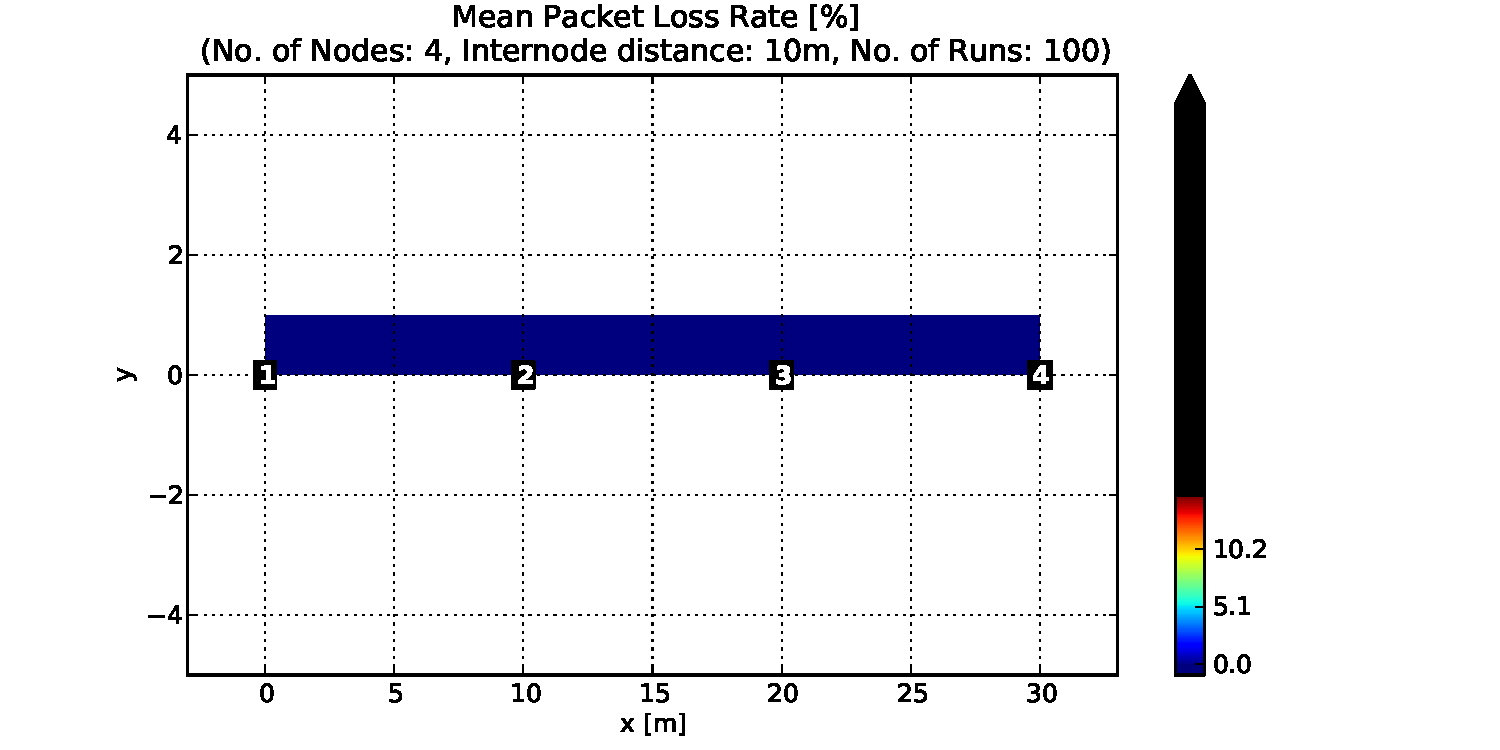
\includegraphics[trim=1.7cm 0cm 3cm 0cm, clip=true, scale=0.38]{Pics/results/4/OF0/line/dist10_montecarlo_contour_packetloss.pdf}}
    \subfloat[MRHOF]{\label{fig:4/MRHOF/line/dist10_montecarlo_contour_packetloss}
      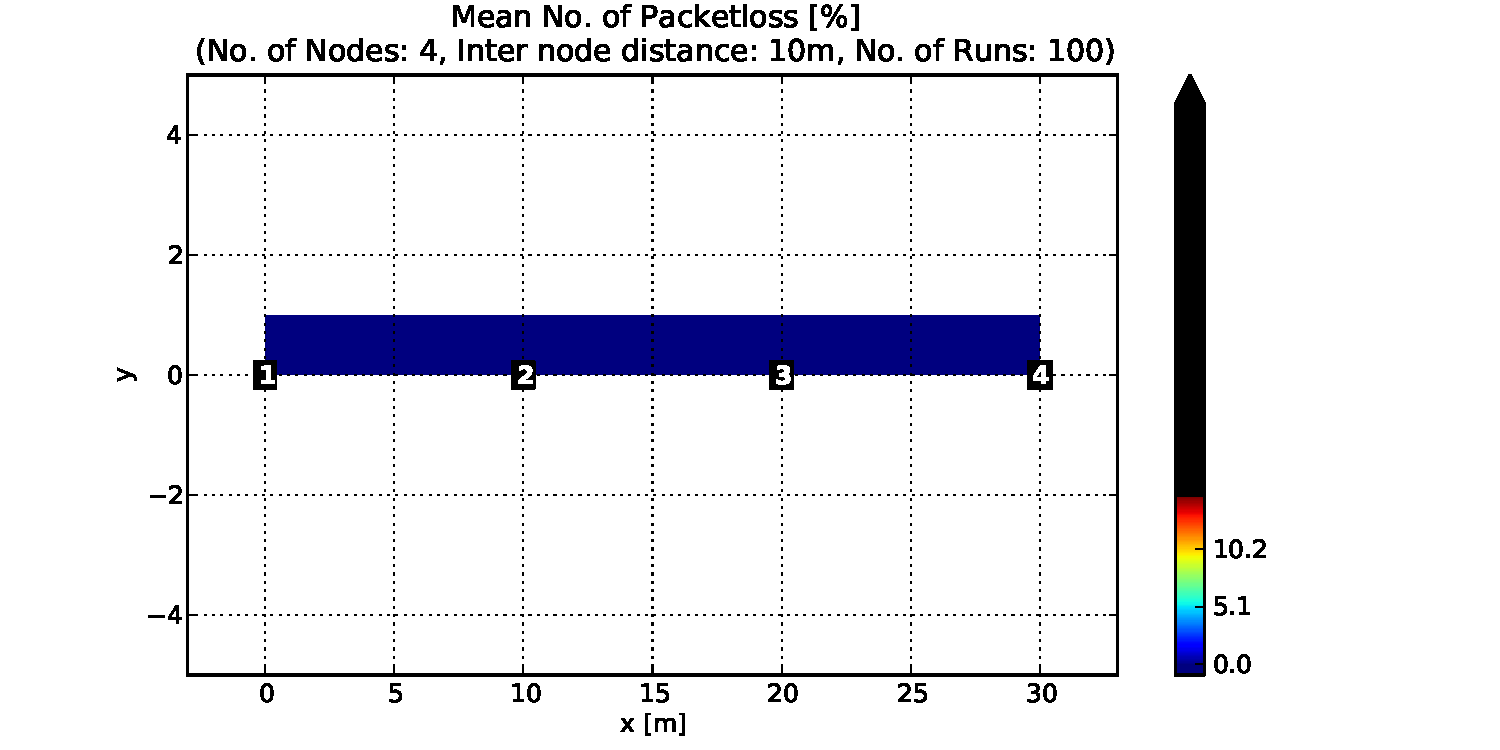
\includegraphics[trim=1.7cm 0cm 3cm 0cm, clip=true, scale=0.38]{Pics/results/4/MRHOF/line/dist10_montecarlo_contour_packetloss.pdf}}
   \caption{Mean packet loss rate: 4-node line scenario with 10 m internode distance}
   \label{fig:pl_4_line_10}
\end{figure}

\begin{figure}[p]
  \centering
    \leavevmode
    \subfloat[OF0]{\label{fig:4/OF0/line/dist50_montecarlo_contour_packetloss}
    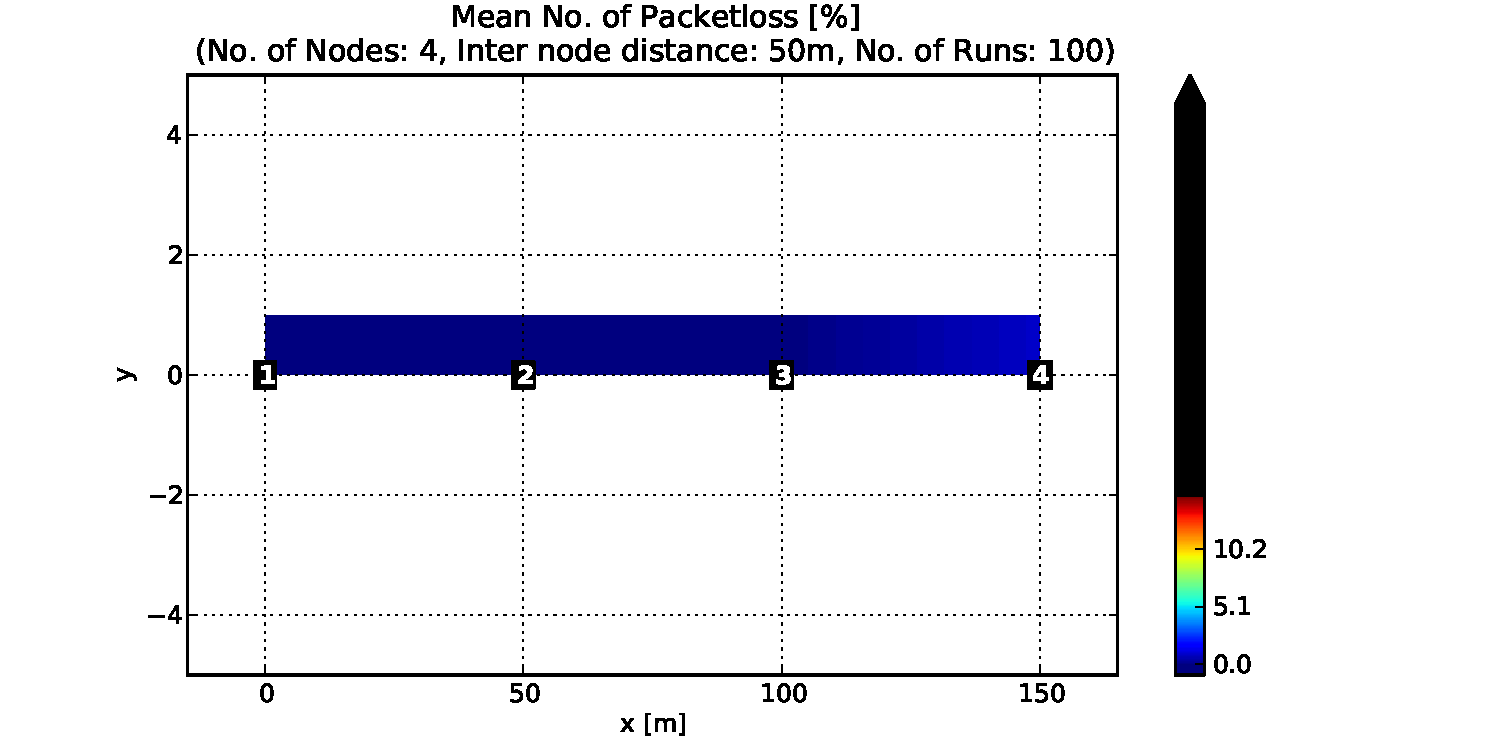
\includegraphics[trim=1.7cm 0cm 3cm 0cm, clip=true, scale=0.38]   {Pics/results/4/OF0/line/dist50_montecarlo_contour_packetloss.pdf}}
    \subfloat[MRHOF]{\label{fig:4/MRHOF/line/dist50_montecarlo_contour_packetloss}
      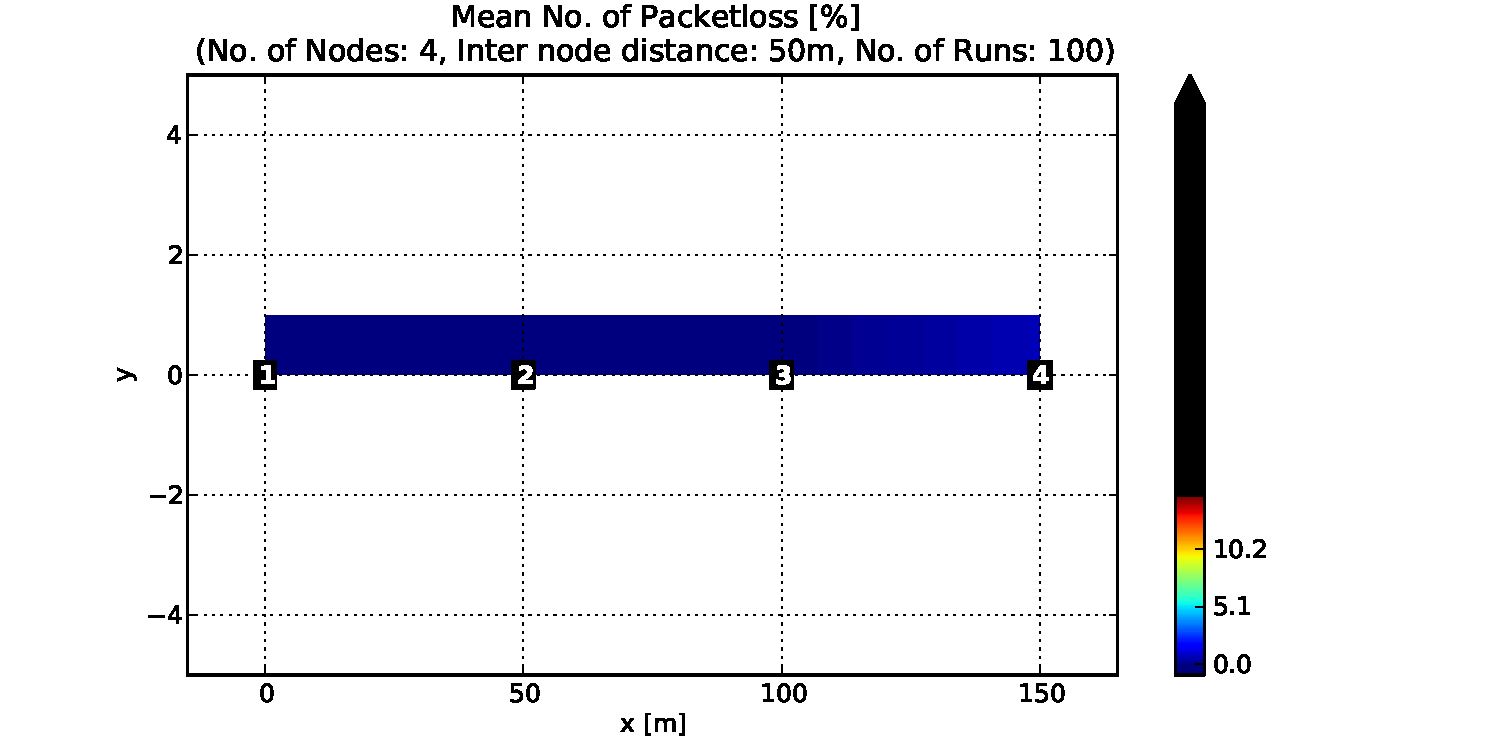
\includegraphics[trim=1.7cm 0cm 3cm 0cm, clip=true, scale=0.38]{Pics/results/4/MRHOF/line/dist50_montecarlo_contour_packetloss.pdf}}
   \caption{Mean packet loss rate: 4-node line scenario with 50 m internode distance}
   \label{fig:pl_4_line_50}
\end{figure}

\begin{figure}[p]
  \centering
    \leavevmode
    \subfloat[OF0]{\label{fig:4/OF0/line/dist100_montecarlo_contour_packetloss}
     \includegraphics[trim=1.7cm 0cm 3cm 0cm, clip=true, scale=0.38]{Pics/results/4/OF0/line/dist100_montecarlo_contour_packetloss.pdf}}
    \subfloat[MRHOF]{\label{fig:4/MRHOF/line/dist100_montecarlo_contour_packetloss}
     \includegraphics[trim=1.7cm 0cm 3cm 0cm, clip=true, scale=0.38]{Pics/results/4/MRHOF/line/dist100_montecarlo_contour_packetloss.pdf}}
  \caption{Mean packet loss rate: 4-node line scenario with 100 m internode distance}
  \label{fig:pl_4_line_100}
\end{figure}
%%%%%%%%%%%%%%%%%%%%%%%%%%%%%%%%%%%%%%% line 9 %%%%%%%%%%%%%%%%%%%%%%%%%%%%%%%%%%%%%%%%
\begin{figure}[p]
  \centering
    \leavevmode
    \subfloat[OF0]{\label{fig:9/OF0/line/dist10_montecarlo_contour_packetloss}
      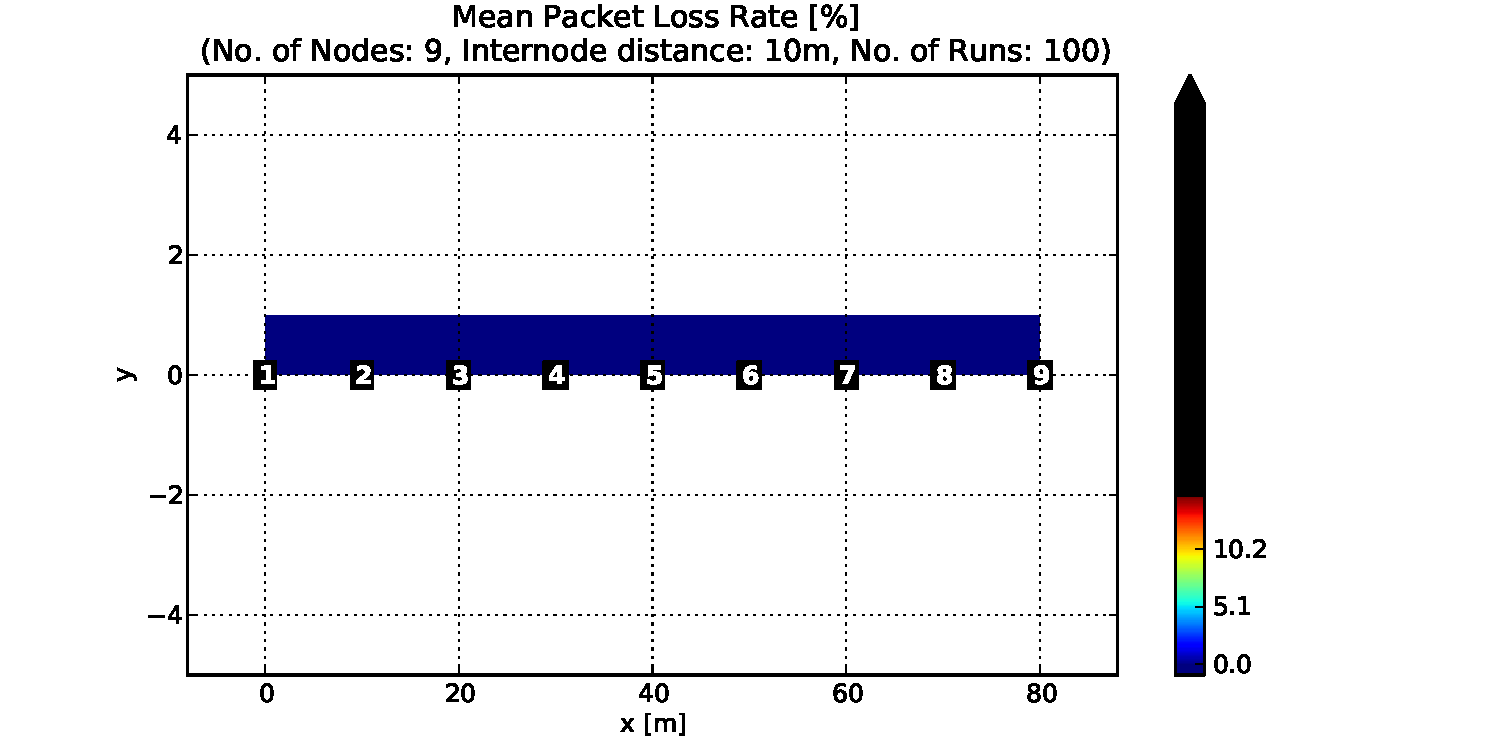
\includegraphics[trim=1.7cm 0cm 3cm 0cm, clip=true, scale=0.38]{Pics/results/9/OF0/line/dist10_montecarlo_contour_packetloss.pdf}}
    \subfloat[MRHOF]{\label{fig:9/MRHOF/line/dist10_montecarlo_contour_packetloss}
      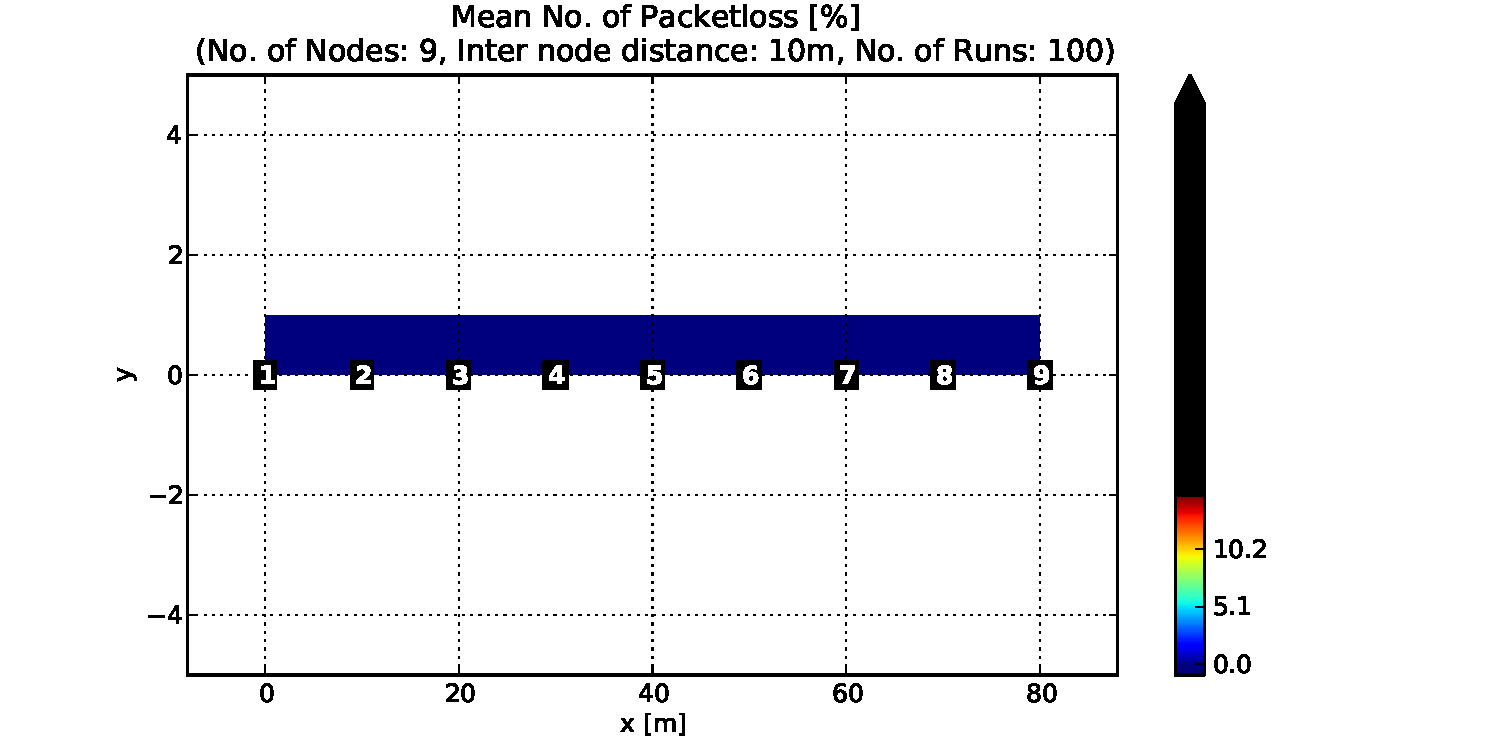
\includegraphics[trim=1.7cm 0cm 3cm 0cm, clip=true, scale=0.38]{Pics/results/9/MRHOF/line/dist10_montecarlo_contour_packetloss.pdf}}
   \caption{Mean packet loss rate: 9-node line scenario with 10 m internode distance}
   \label{fig:pl_9_line_10}
\end{figure}

\begin{figure}[p]
  \centering
    \leavevmode
    \subfloat[OF0]{\label{fig:9/OF0/line/dist50_montecarlo_contour_packetloss}
    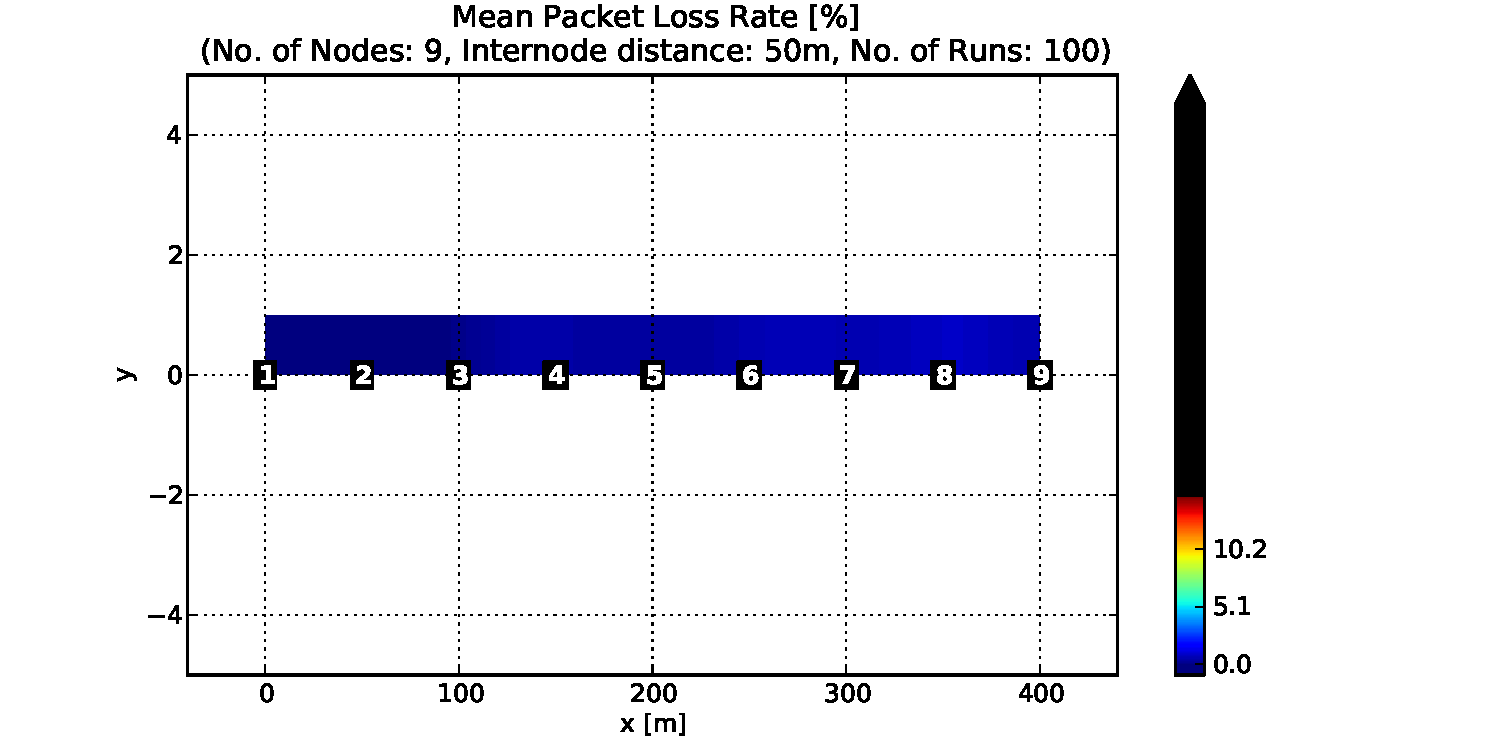
\includegraphics[trim=1.7cm 0cm 3cm 0cm, clip=true, scale=0.38]   {Pics/results/9/OF0/line/dist50_montecarlo_contour_packetloss.pdf}}
    \subfloat[MRHOF]{\label{fig:9/MRHOF/line/dist50_montecarlo_contour_packetloss}
      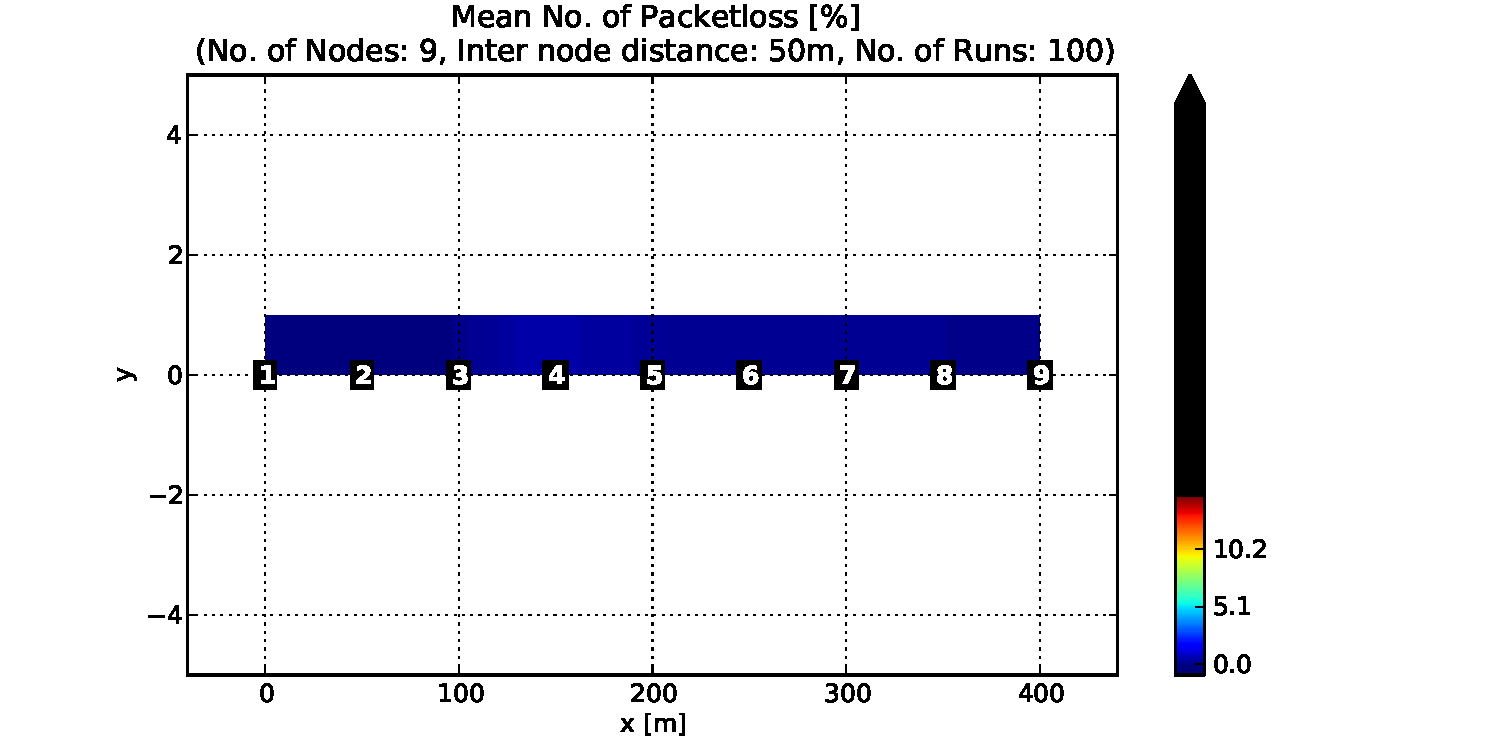
\includegraphics[trim=1.7cm 0cm 3cm 0cm, clip=true, scale=0.38]{Pics/results/9/MRHOF/line/dist50_montecarlo_contour_packetloss.pdf}}
   \caption{Mean packet loss rate: 9-node line scenario with 50 m internode distance}
   \label{fig:pl_9_line_50}
\end{figure}

\begin{figure}[p]
  \centering
    \leavevmode
    \subfloat[OF0]{\label{fig:9/OF0/line/dist100_montecarlo_contour_packetloss}
     \includegraphics[trim=1.7cm 0cm 3cm 0cm, clip=true, scale=0.38]{Pics/results/9/OF0/line/dist100_montecarlo_contour_packetloss.pdf}}
    \subfloat[MRHOF]{\label{fig:9/MRHOF/line/dist100_montecarlo_contour_packetloss}
     \includegraphics[trim=1.7cm 0cm 3cm 0cm, clip=true, scale=0.38]{Pics/results/9/MRHOF/line/dist100_montecarlo_contour_packetloss.pdf}}
  \caption{Mean packet loss rate: 9-node line scenario with 100 m internode distance}
  \label{fig:pl_9_line_100}
\end{figure}

%%%%%%%%%%%%%%%%%%%%%%%%%%%%%%%%%%%%%%% line 16 %%%%%%%%%%%%%%%%%%%%%%%%%%%%%%%%%%%%%%%%

\begin{figure}[p]
  \centering
    \leavevmode
    \subfloat[OF0]{\label{fig:16/OF0/line/dist10_montecarlo_contour_packetloss}
      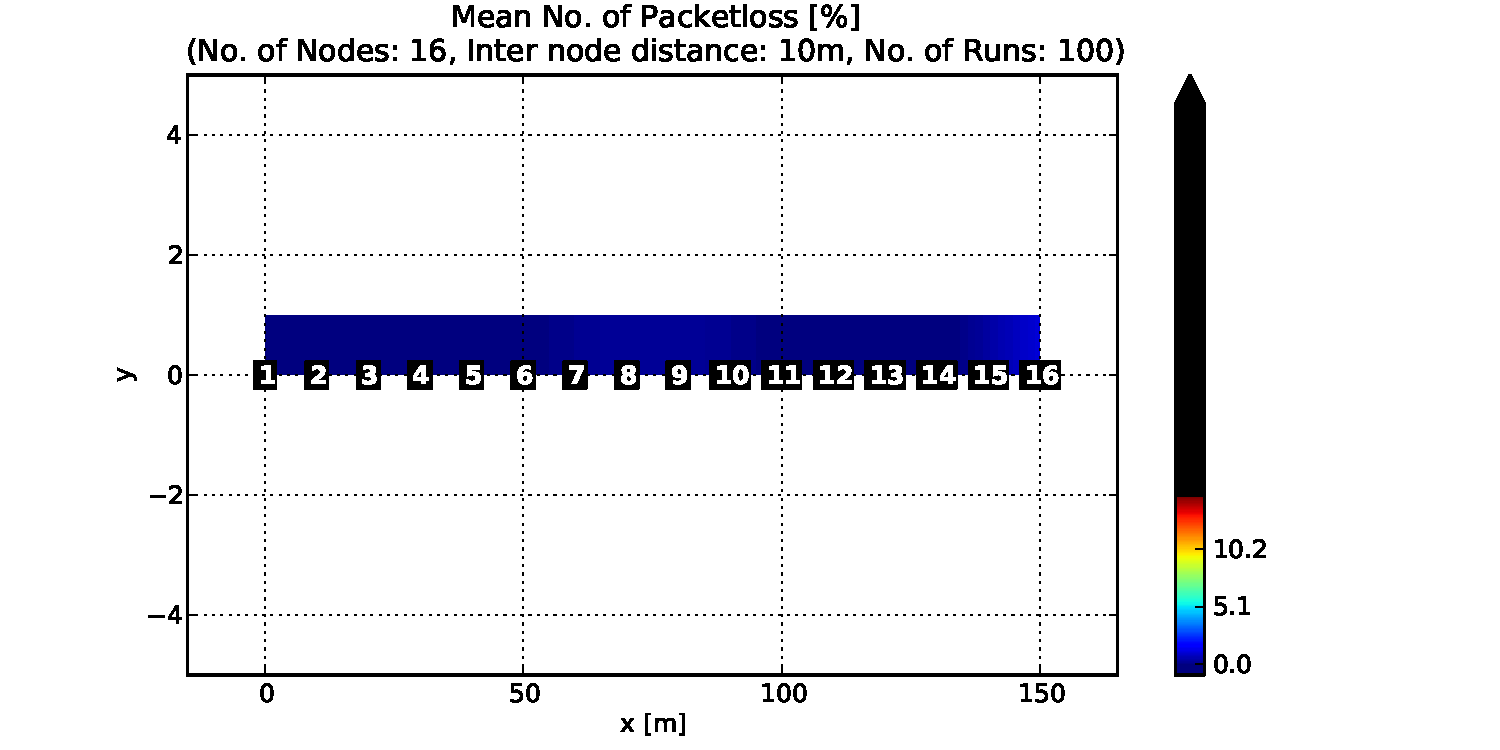
\includegraphics[trim=1.7cm 0cm 3cm 0cm, clip=true, scale=0.38]{Pics/results/16/OF0/line/dist10_montecarlo_contour_packetloss.pdf}}
    \subfloat[MRHOF]{\label{fig:16/MRHOF/line/dist10_montecarlo_contour_packetloss}
      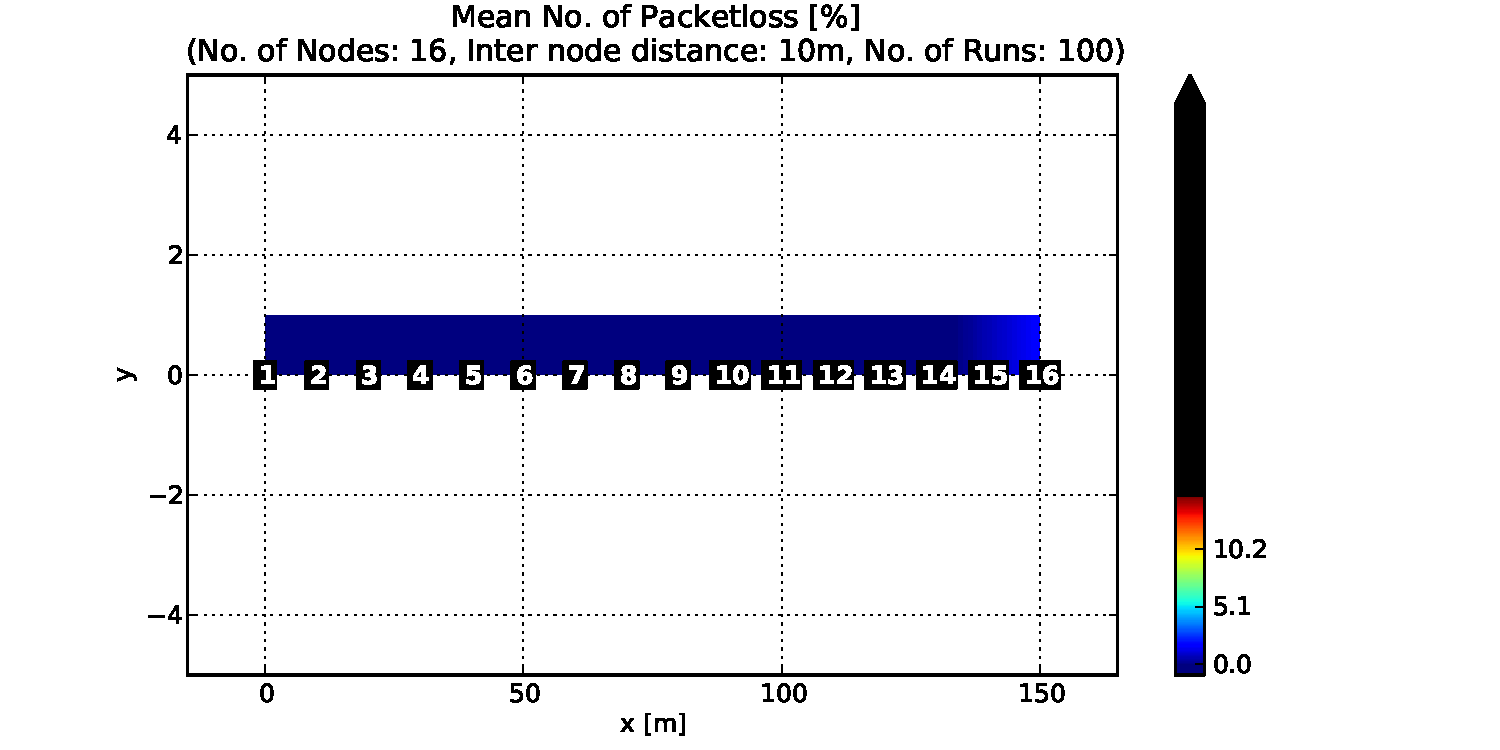
\includegraphics[trim=1.7cm 0cm 3cm 0cm, clip=true, scale=0.38]{Pics/results/16/MRHOF/line/dist10_montecarlo_contour_packetloss.pdf}}
   \caption{Mean packet loss rate: 16-node line scenario with 10 m internode distance}
   \label{fig:pl_16_line_10}
\end{figure}

\begin{figure}[p]
  \centering
    \leavevmode
    \subfloat[OF0]{\label{fig:16/OF0/line/dist50_montecarlo_contour_packetloss}
    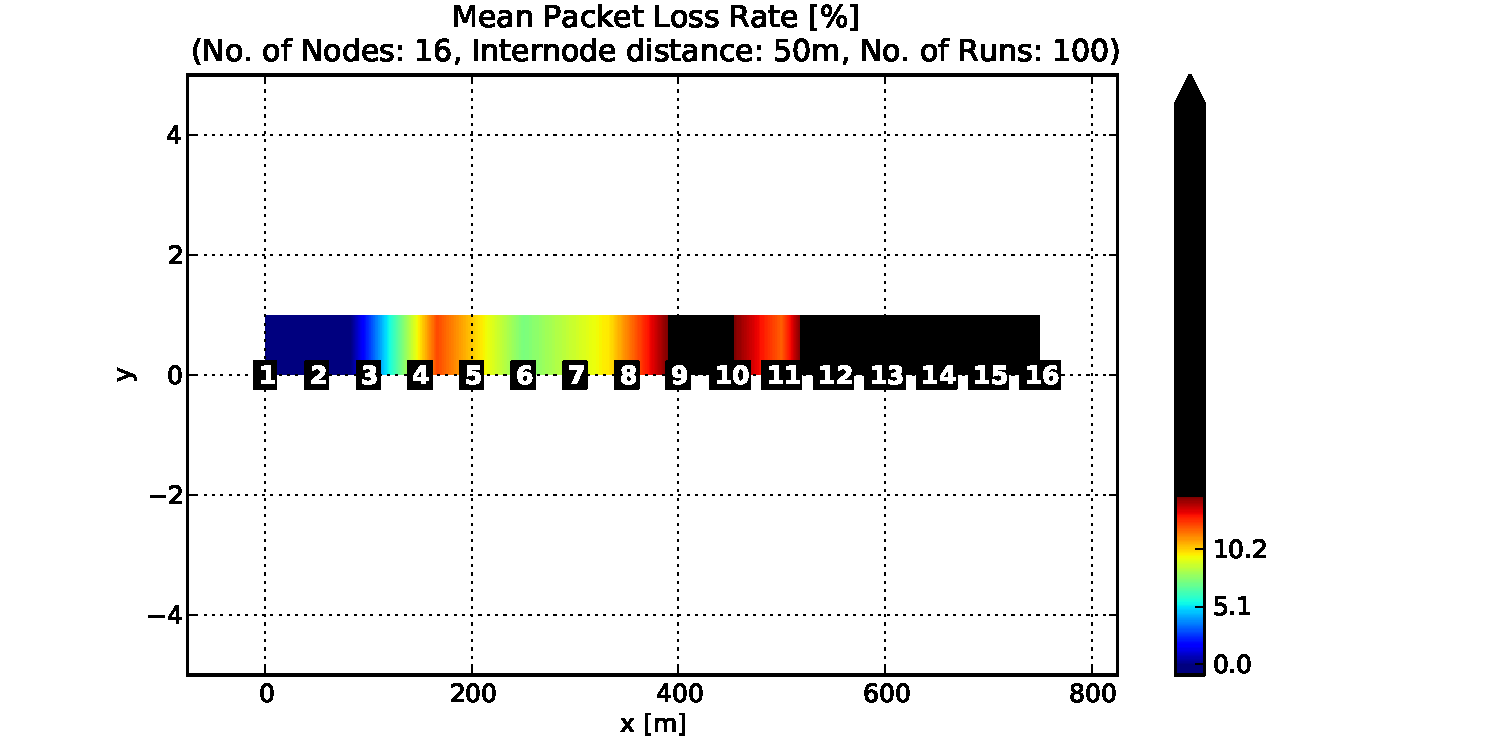
\includegraphics[trim=1.7cm 0cm 3cm 0cm, clip=true, scale=0.38]   {Pics/results/16/OF0/line/dist50_montecarlo_contour_packetloss.pdf}}
    \subfloat[MRHOF]{\label{fig:16/MRHOF/line/dist50_montecarlo_contour_packetloss}
      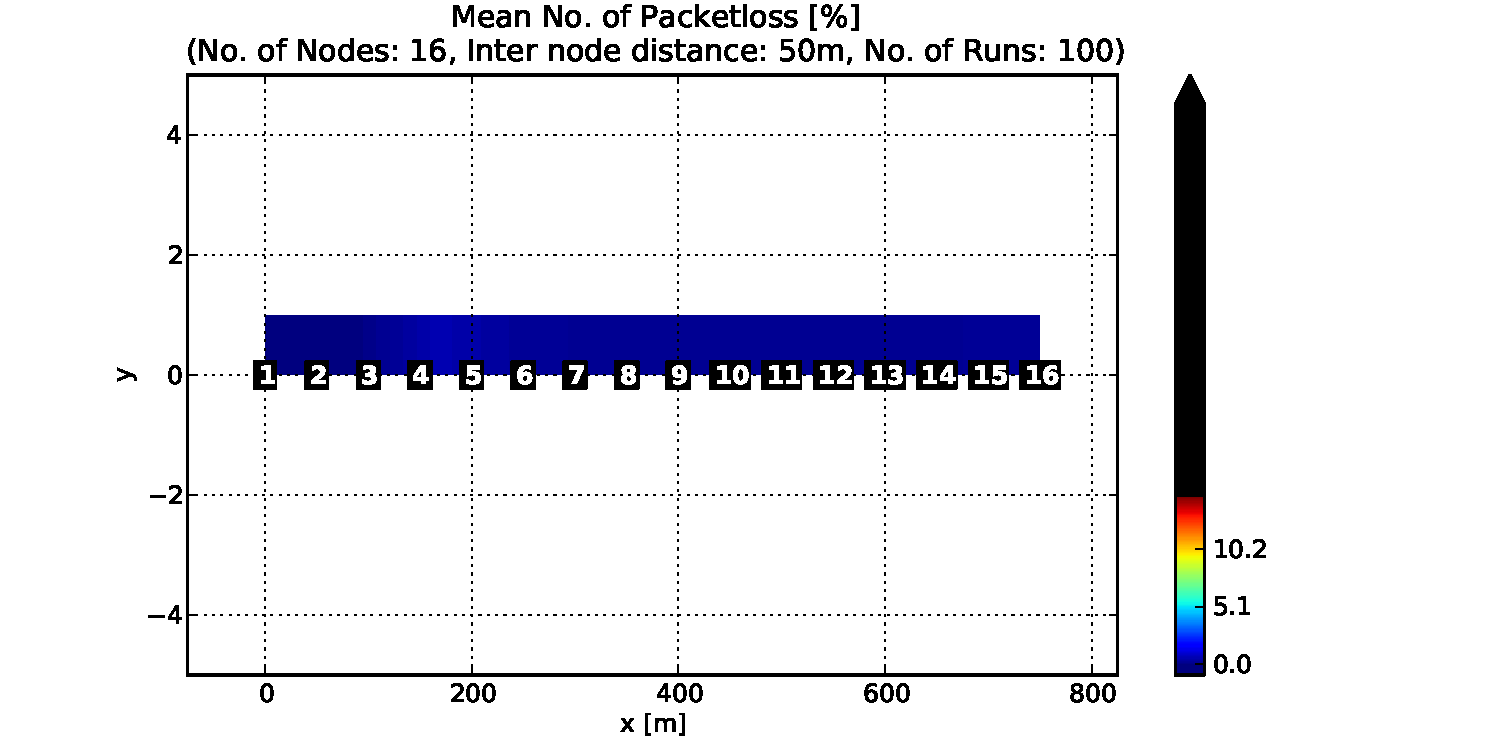
\includegraphics[trim=1.7cm 0cm 3cm 0cm, clip=true, scale=0.38]{Pics/results/16/MRHOF/line/dist50_montecarlo_contour_packetloss.pdf}}
   \caption{Mean packet loss rate: 16-node line scenario with 50 m internode distance}
   \label{fig:pl_16_line_50}
\end{figure}

\begin{figure}[p]
  \centering
    \leavevmode
    \subfloat[OF0]{\label{fig:16/OF0/line/dist100_montecarlo_contour_packetloss}
     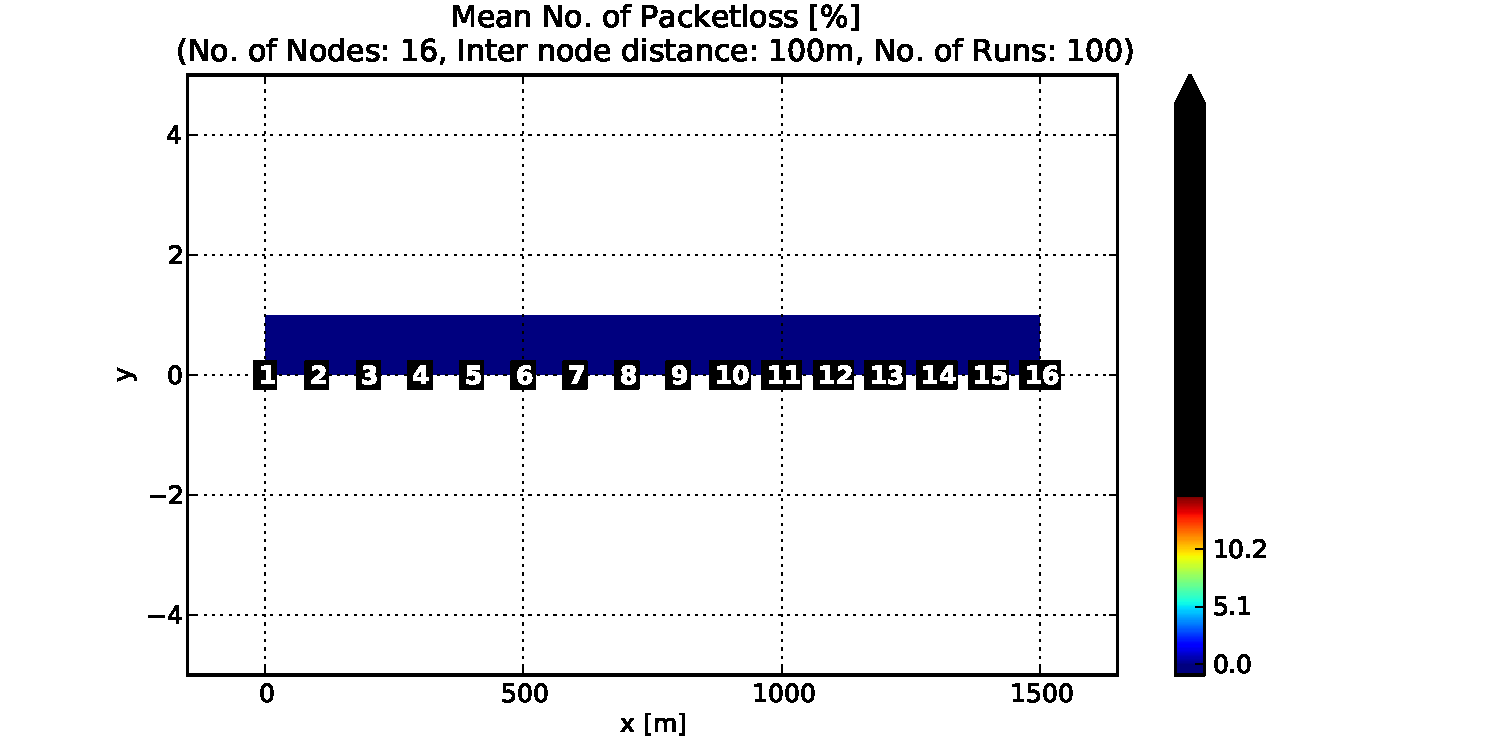
\includegraphics[trim=1.7cm 0cm 3cm 0cm, clip=true, scale=0.38]{Pics/results/16/OF0/line/dist100_montecarlo_contour_packetloss.pdf}}
    \subfloat[MRHOF]{\label{fig:16/MRHOF/line/dist100_montecarlo_contour_packetloss}
     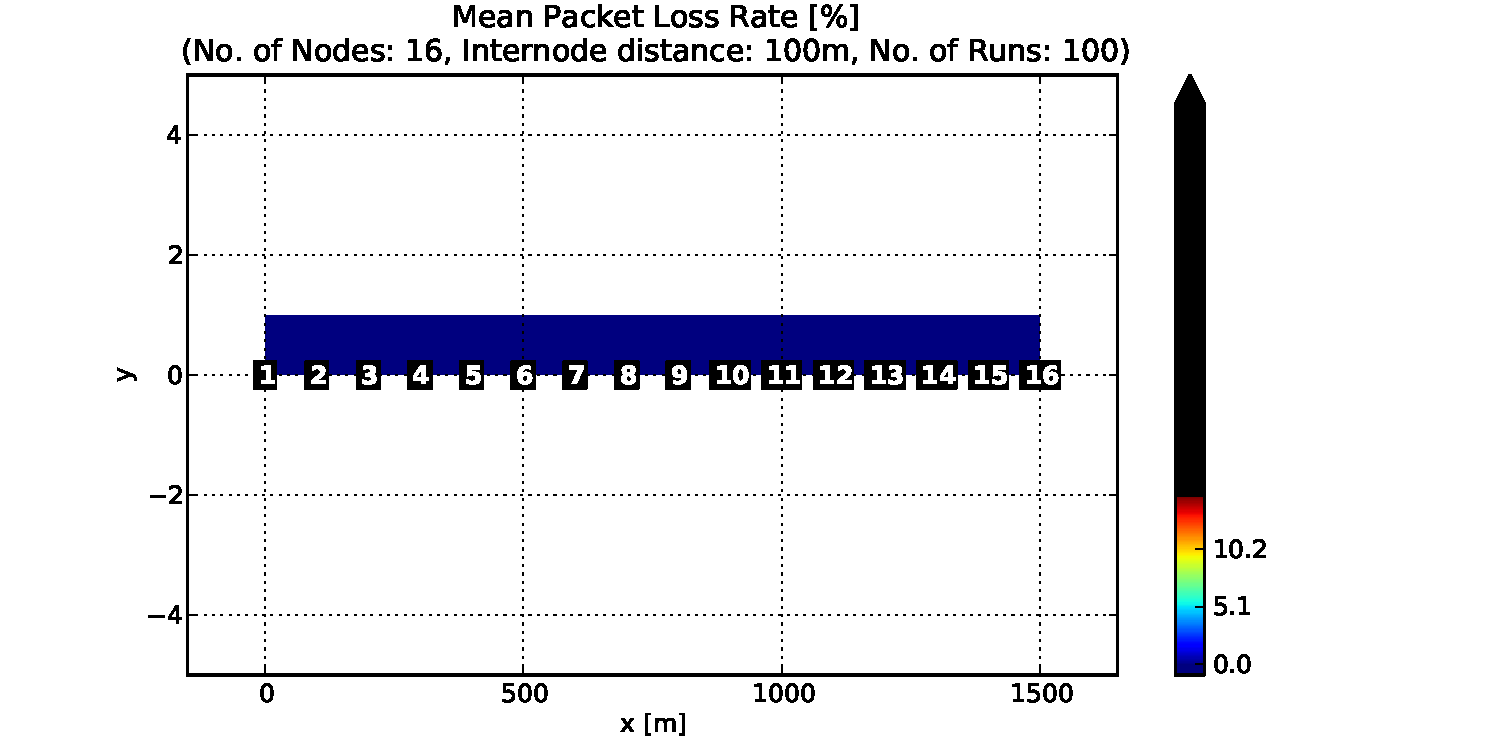
\includegraphics[trim=1.7cm 0cm 3cm 0cm, clip=true, scale=0.38]{Pics/results/16/MRHOF/line/dist100_montecarlo_contour_packetloss.pdf}}
  \caption{Mean packet loss rate: 16-node line scenario with 100 m internode distance}
  \label{fig:pl_16_line_100}
\end{figure}

For the 4-node and 9-node line scenarios, the packet loss under the same setup shows no difference between OF0 and MRHOF. When the node number increases to 16, simulation with OF0 starts to exhibit a higher packet loss than MRHOF. In the 50 meters internode distance case (Figure \ref{fig:16/OF0/line/dist50_montecarlo_contour_packetloss}), one can see a mean packet loss rate higher than 15\% for the most distant nodes. This result is caused either by broken routes, or by a low PRR between the root and the nodes in one or more runs of the 100 runs. When the internode distance increased to 100 meters, OF0 presents again a good case in terms of packet loss rate (Figure \ref{fig:16/OF0/line/dist100_montecarlo_contour_packetloss}). In the meanwhile, MRHOF continues to show a stable result over all runs.   
\newline 

\subsection{Grid Scenario}
\label{pl:grid}
The mean packet loss rate results for grid scenario are shown in Figure \ref{fig:pl_4_grid_10} to Figure \ref{fig:pl_16_grid_100}.

%%%%%%%%%%%%%%%%%%%%%%%%%%%%%%%%%%%%%%% grid 4 %%%%%%%%%%%%%%%%%%%%%%%%%%%%%%%%%%%%%%%%
\begin{figure}[p]
  \centering
    \leavevmode
    \subfloat[OF0]{\label{fig:4/OF0/grid/dist10_montecarlo_contour_packetloss}
      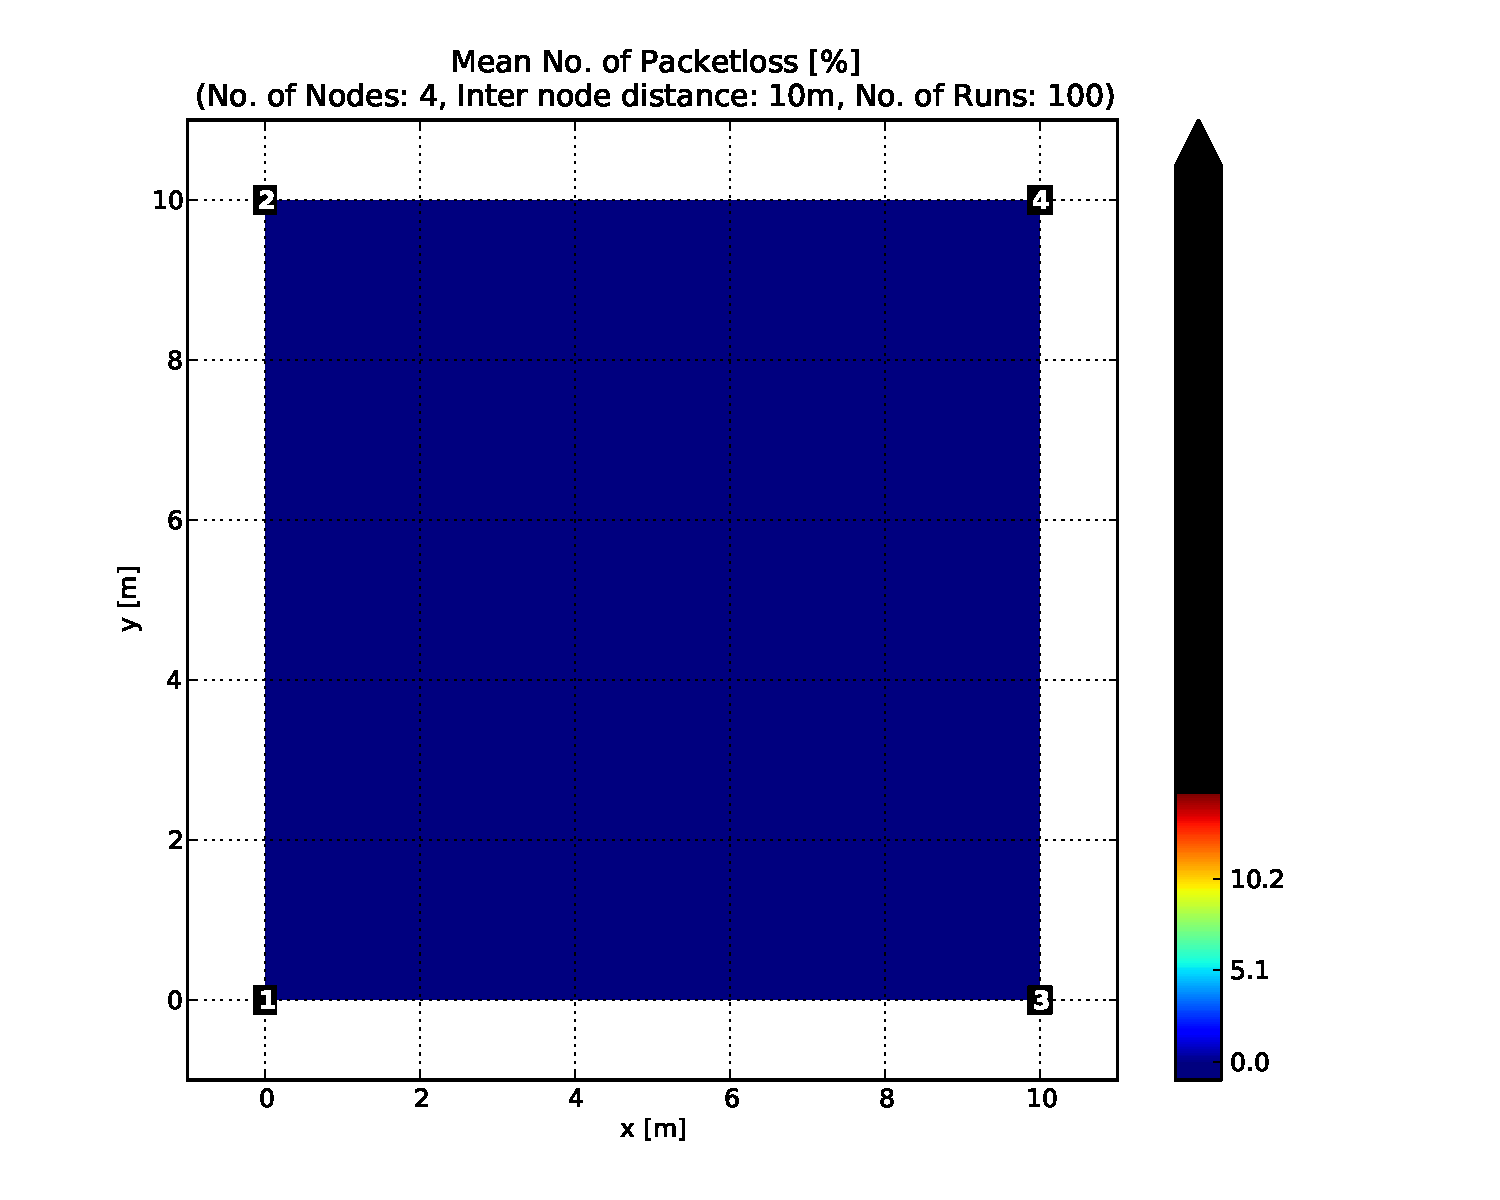
\includegraphics[trim=1.7cm 0cm 3cm 0cm, clip=true, scale=0.38]{Pics/results/4/OF0/grid/dist10_montecarlo_contour_packetloss.pdf}}
    \subfloat[MRHOF]{\label{fig:4/MRHOF/grid/dist10_montecarlo_contour_packetloss}
      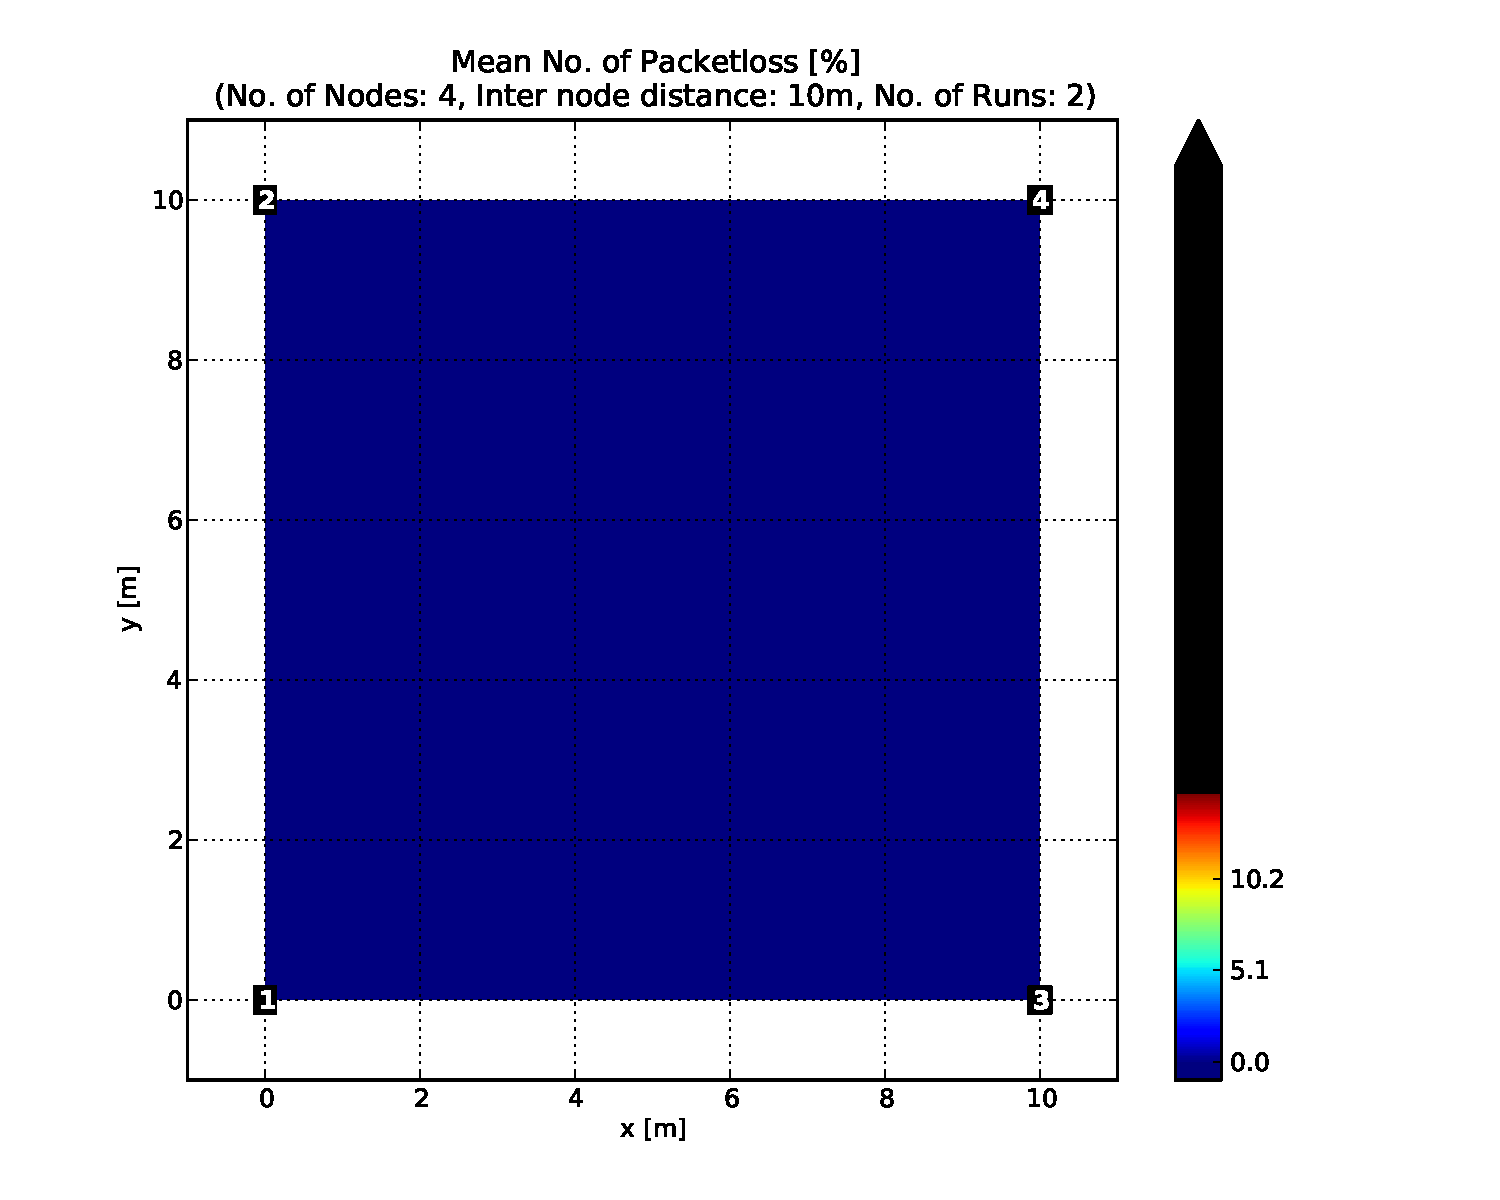
\includegraphics[trim=1.7cm 0cm 3cm 0cm, clip=true, scale=0.38]{Pics/results/4/MRHOF/grid/dist10_montecarlo_contour_packetloss.pdf}}
   \caption{Mean packet loss rate: 4-node grid scenario with 10 m internode distance}
   \label{fig:pl_4_grid_10}
\end{figure}

\begin{figure}[p]
  \centering
    \leavevmode
    \subfloat[OF0]{\label{fig:4/OF0/grid/dist50_montecarlo_contour_packetloss}
    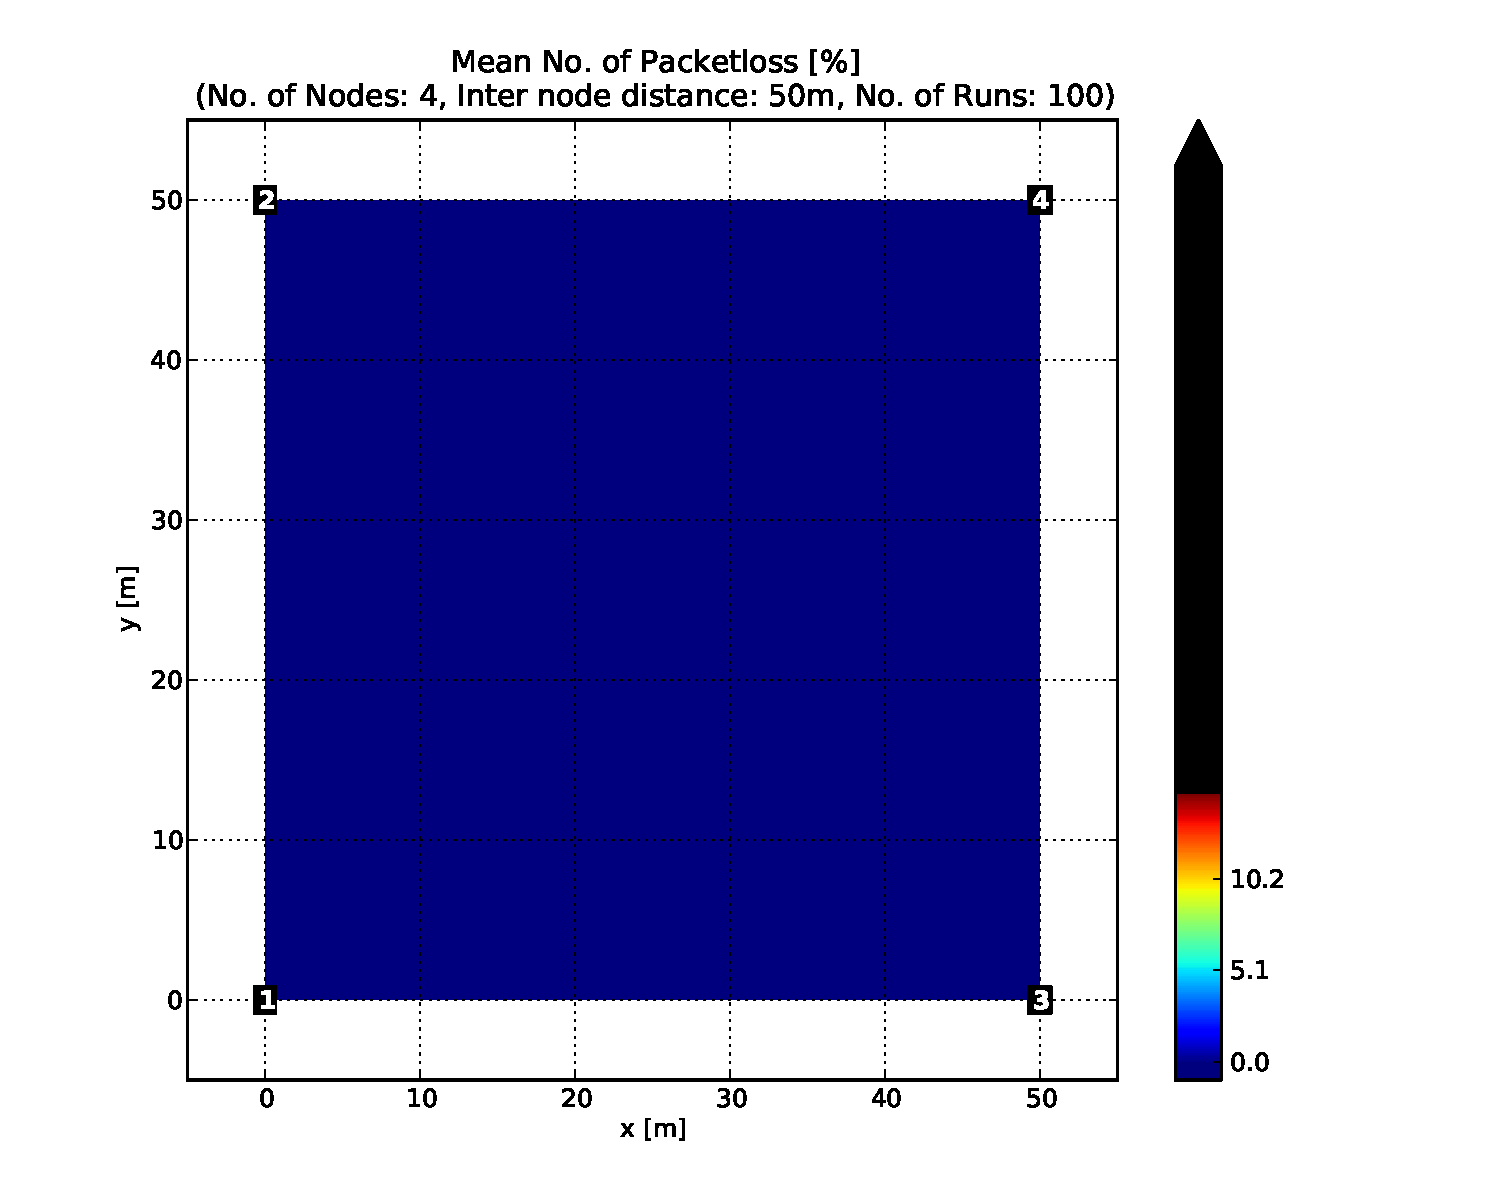
\includegraphics[trim=1.7cm 0cm 3cm 0cm, clip=true, scale=0.38]   {Pics/results/4/OF0/grid/dist50_montecarlo_contour_packetloss.pdf}}
    \subfloat[MRHOF]{\label{fig:4/MRHOF/grid/dist50_montecarlo_contour_packetloss}
      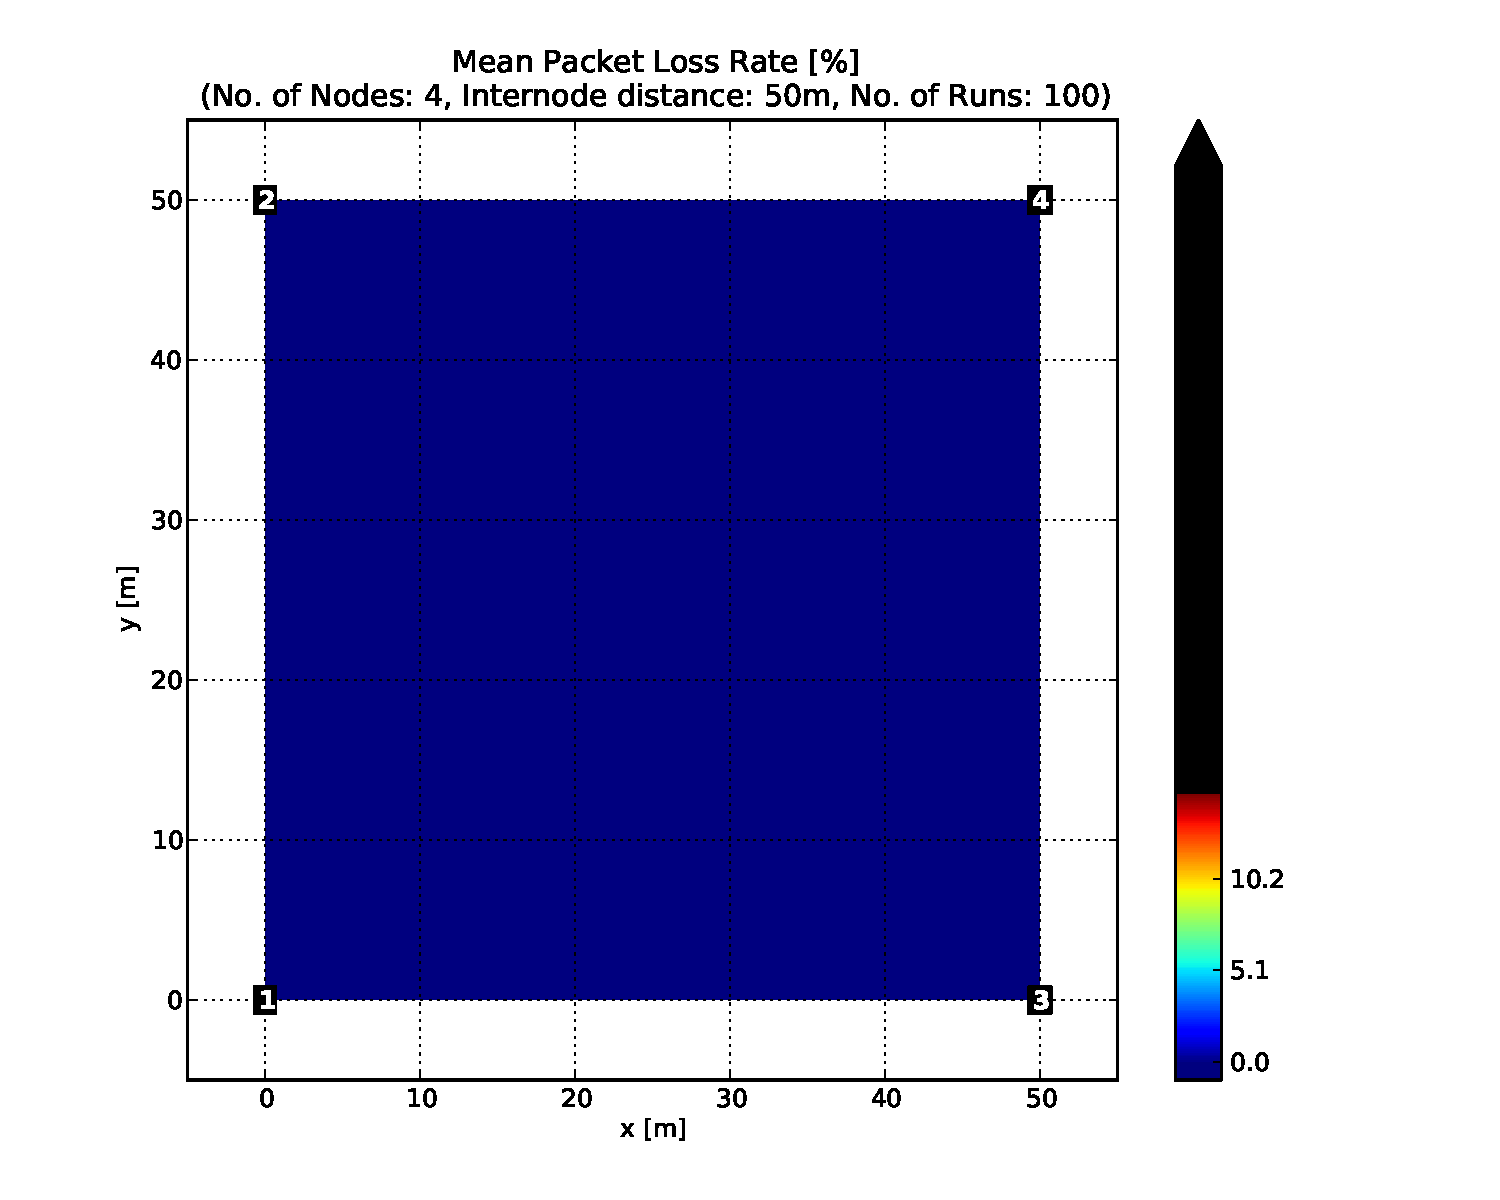
\includegraphics[trim=1.7cm 0cm 3cm 0cm, clip=true, scale=0.38]{Pics/results/4/MRHOF/grid/dist50_montecarlo_contour_packetloss.pdf}}
   \caption{Mean packet loss rate: 4-node grid scenario with 50 m internode distance}
   \label{fig:pl_4_grid_50}
\end{figure}

\begin{figure}[p]
  \centering
    \leavevmode
    \subfloat[OF0]{\label{fig:4/OF0/grid/dist100_montecarlo_contour_packetloss}
     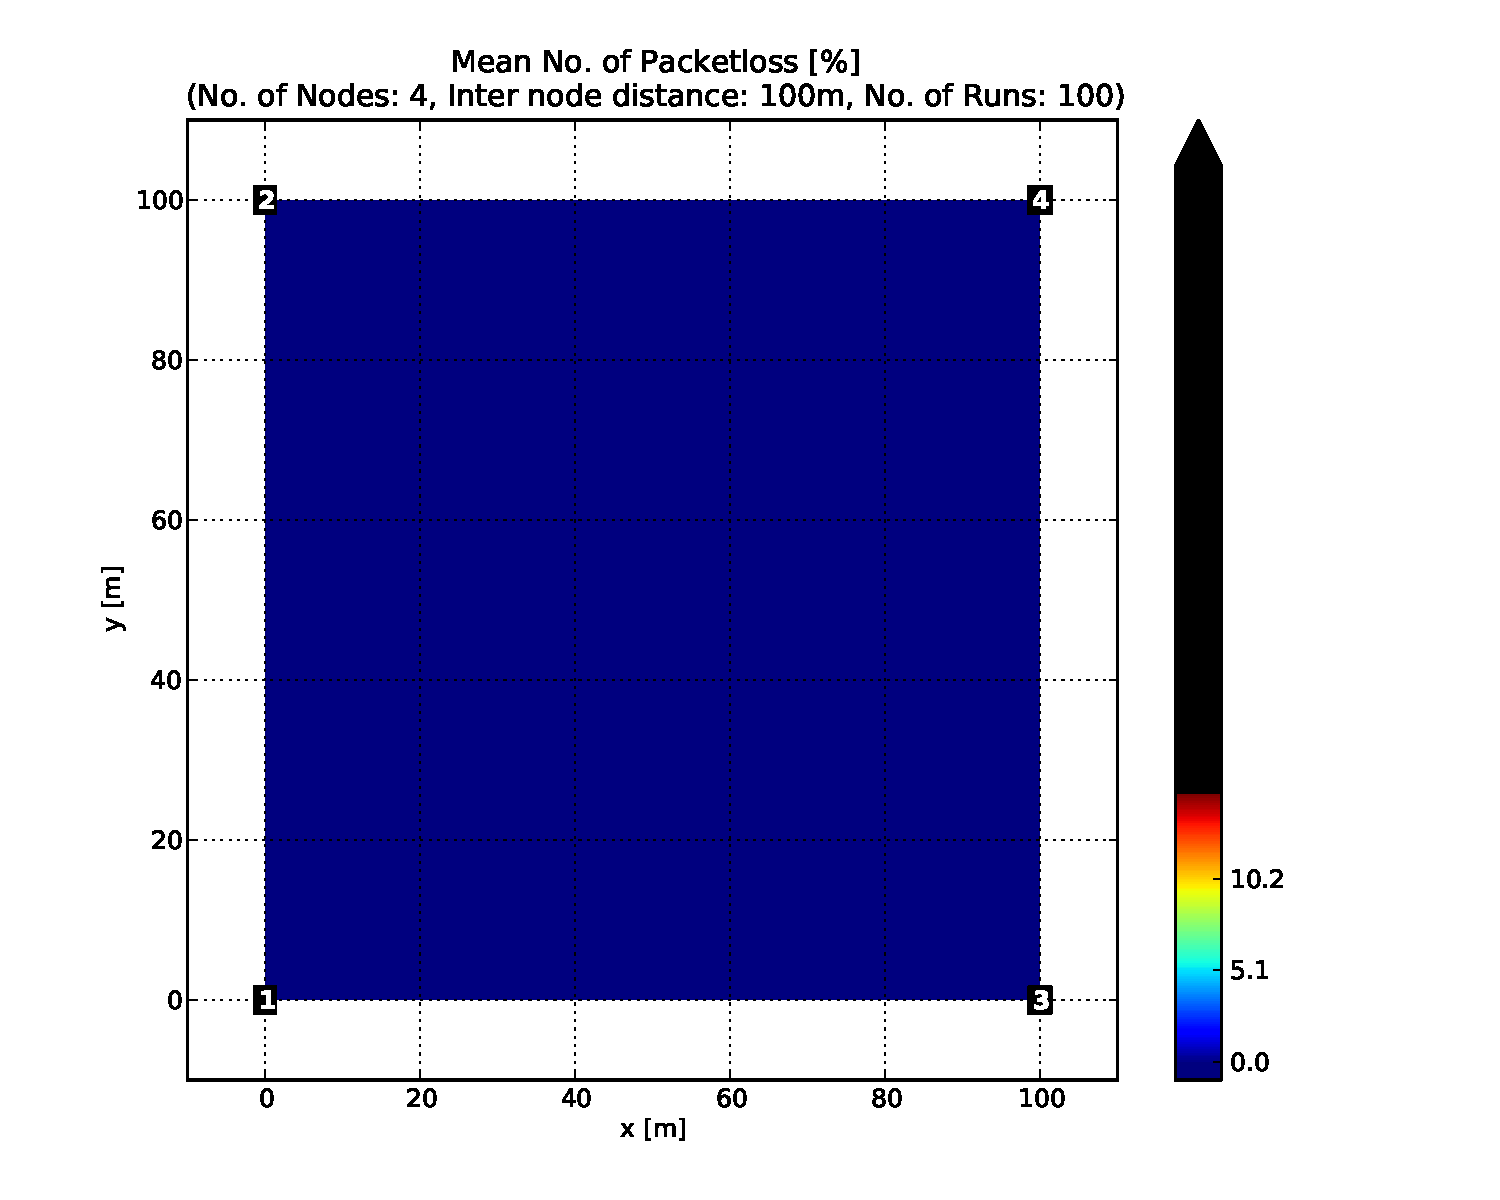
\includegraphics[trim=1.7cm 0cm 3cm 0cm, clip=true, scale=0.38]{Pics/results/4/OF0/grid/dist100_montecarlo_contour_packetloss.pdf}}
    \subfloat[MRHOF]{\label{fig:4/MRHOF/grid/dist100_montecarlo_contour_packetloss}
     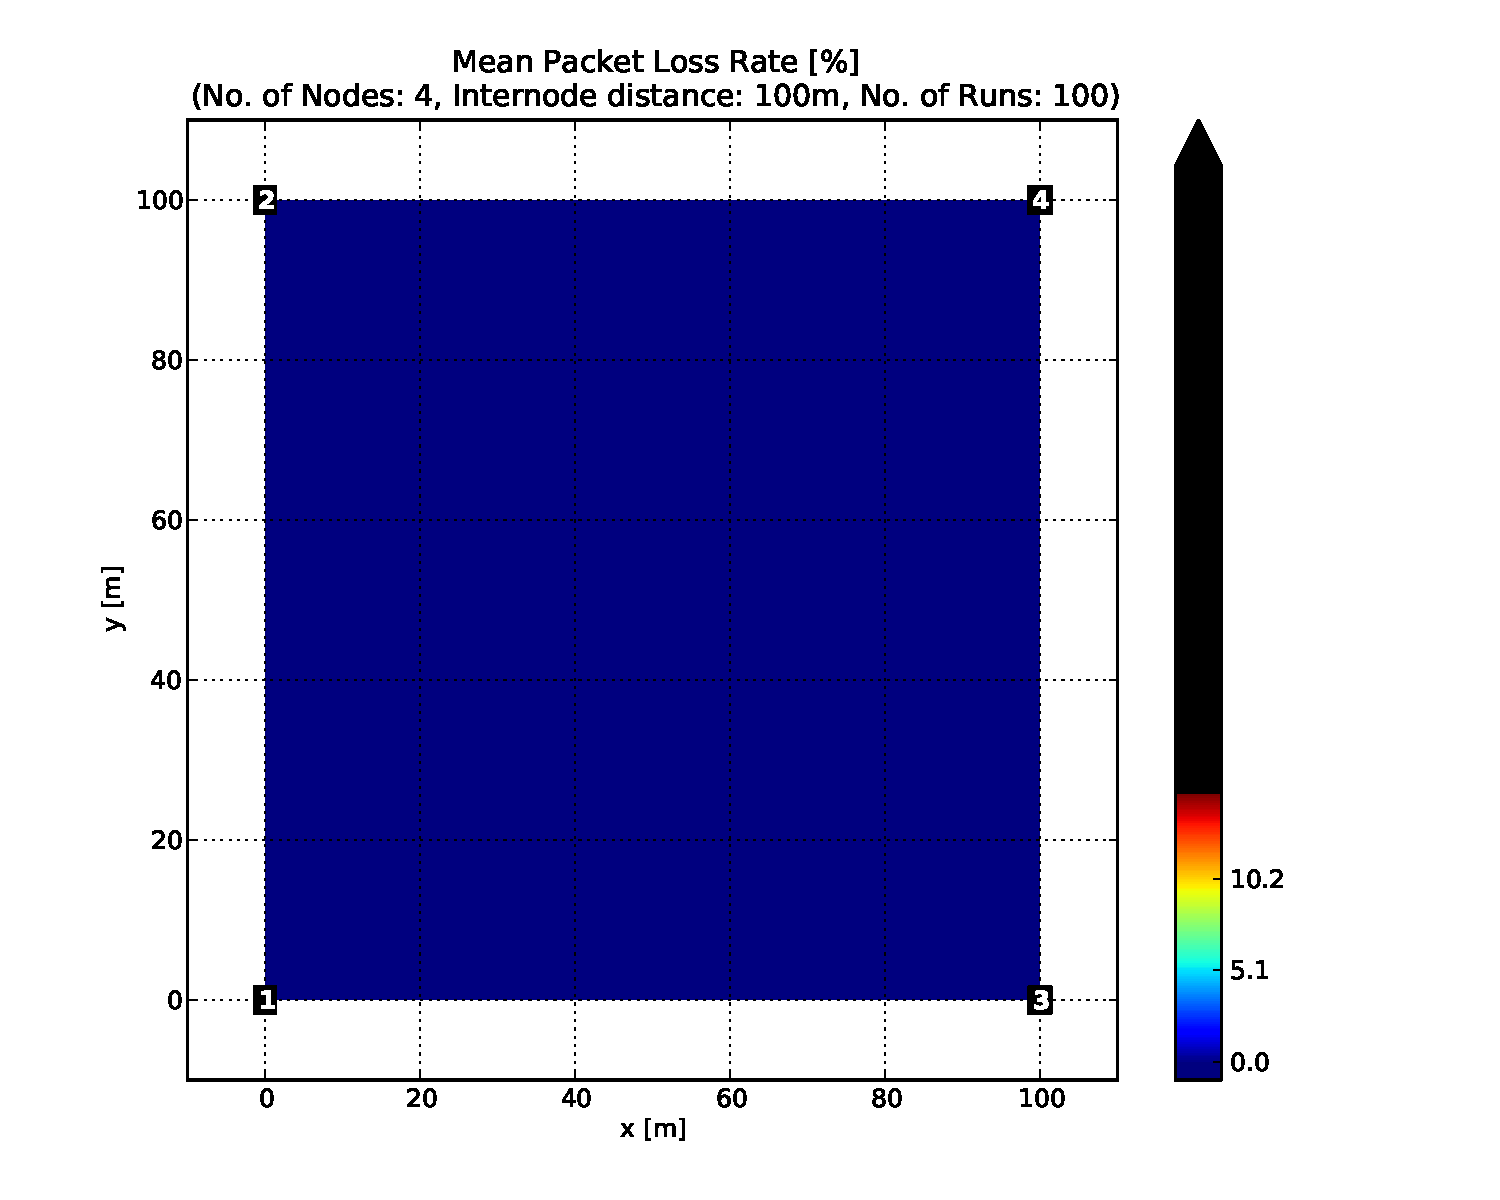
\includegraphics[trim=1.7cm 0cm 3cm 0cm, clip=true, scale=0.38]{Pics/results/4/MRHOF/grid/dist100_montecarlo_contour_packetloss.pdf}}
  \caption{Mean packet loss rate: 4-node grid scenario with 100 m internode distance}
  \label{fig:pl_4_grid_100}
\end{figure}

%%%%%%%%%%%%%%%%%%%%%%%%%%%%%%%%%%%%%%% grid 9 %%%%%%%%%%%%%%%%%%%%%%%%%%%%%%%%%%%%%%%%

\begin{figure}[p]
  \centering
    \leavevmode
    \subfloat[OF0]{\label{fig:9/OF0/grid/dist10_montecarlo_contour_packetloss}
      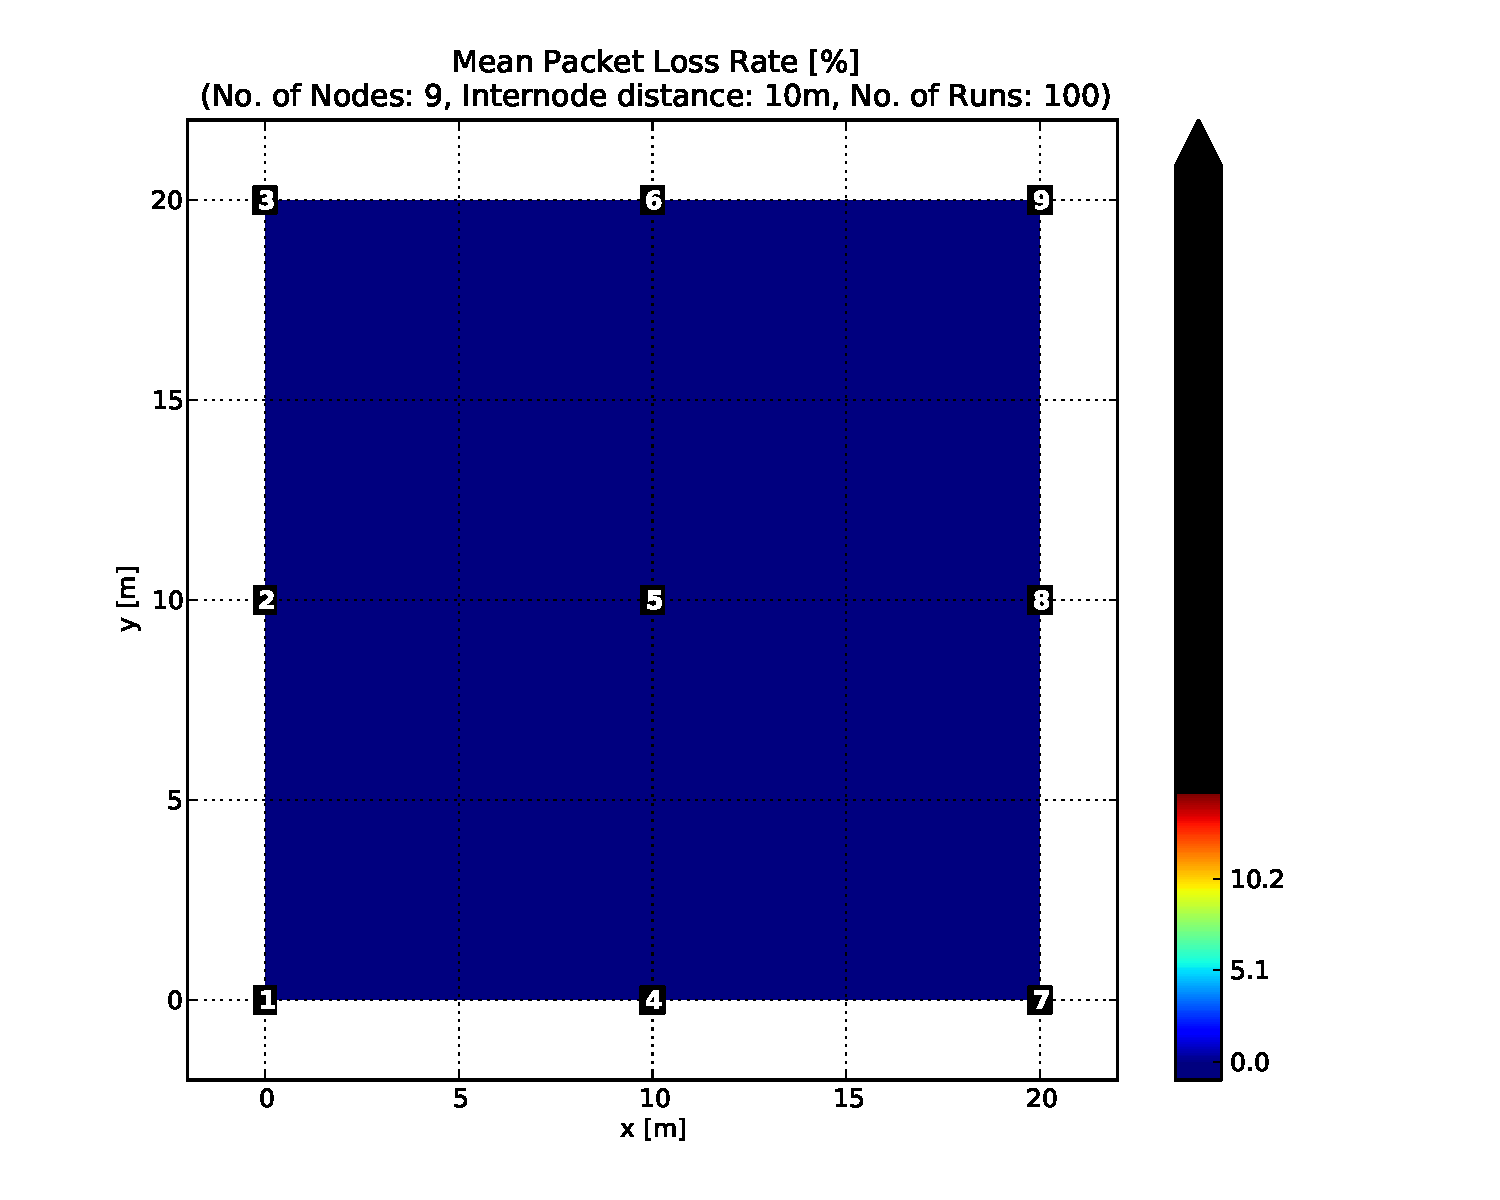
\includegraphics[trim=1.7cm 0cm 3cm 0cm, clip=true, scale=0.38]{Pics/results/9/OF0/grid/dist10_montecarlo_contour_packetloss.pdf}}
    \subfloat[MRHOF]{\label{fig:9/MRHOF/grid/dist10_montecarlo_contour_packetloss}
      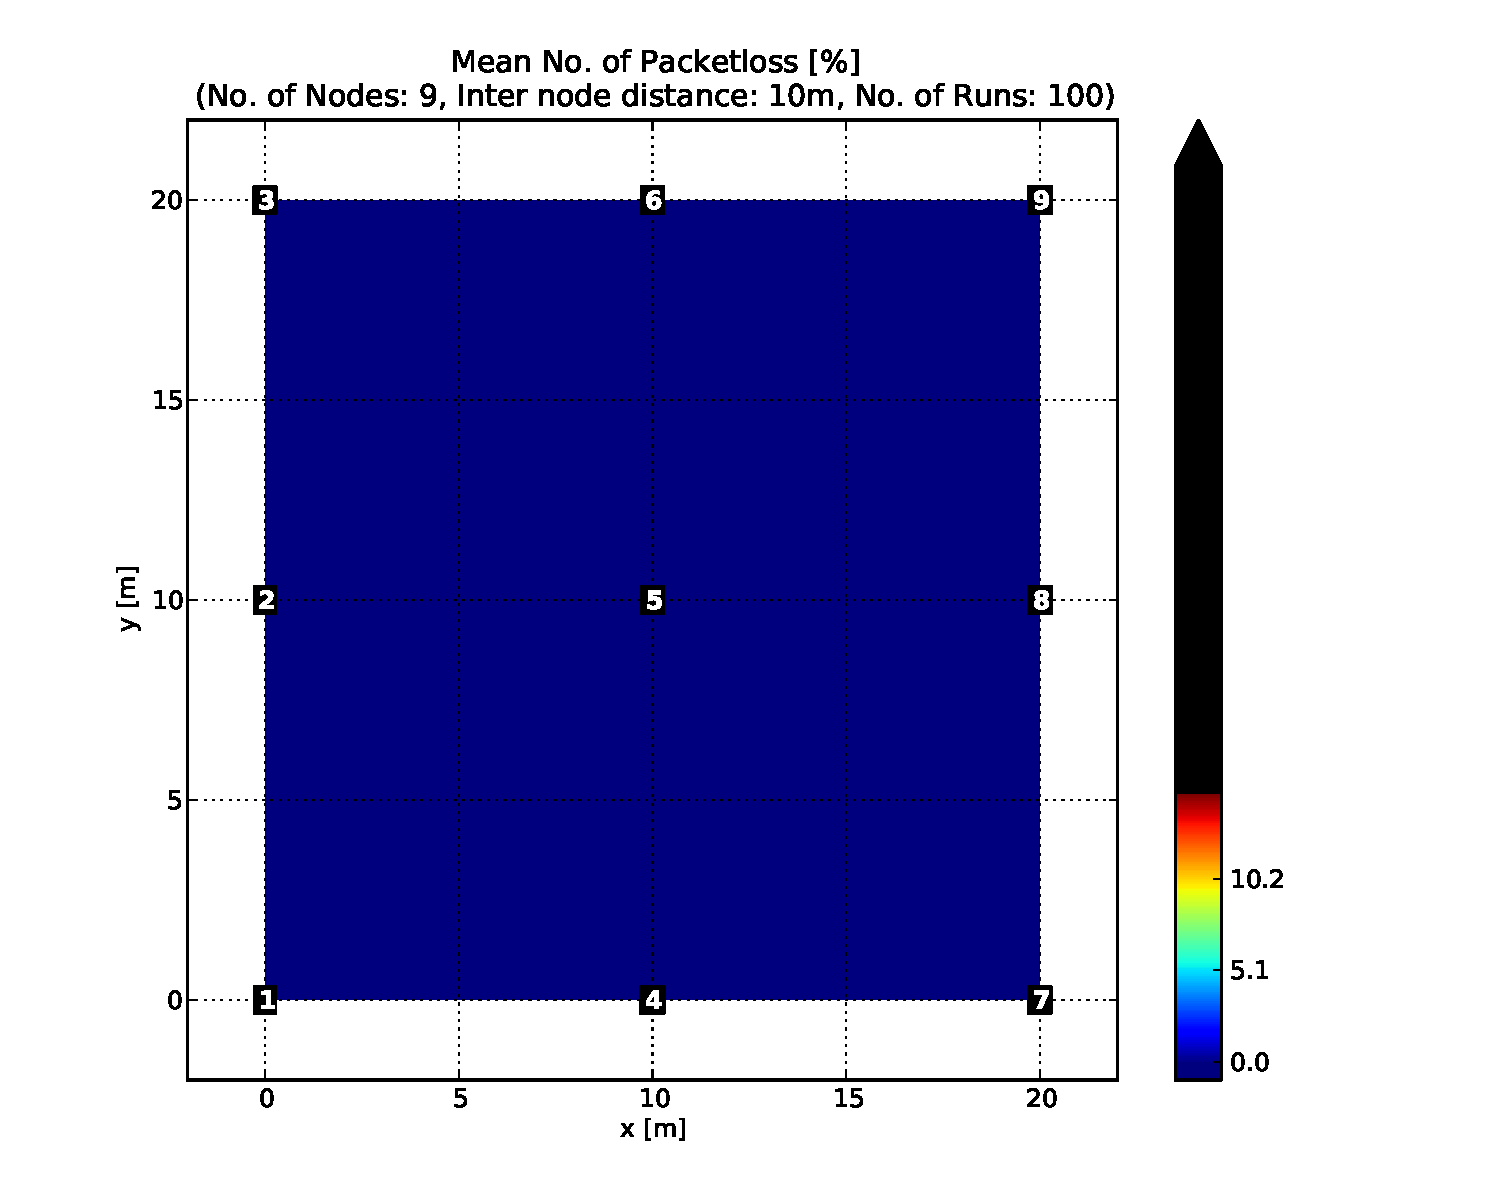
\includegraphics[trim=1.7cm 0cm 3cm 0cm, clip=true, scale=0.38]{Pics/results/9/MRHOF/grid/dist10_montecarlo_contour_packetloss.pdf}}
   \caption{Mean packet loss rate: 9-node grid scenario with 10 m internode distance}
   \label{fig:pl_9_grid_10}
\end{figure}

\begin{figure}[p]
  \centering
    \leavevmode
    \subfloat[OF0]{\label{fig:9/OF0/grid/dist50_montecarlo_contour_packetloss}
    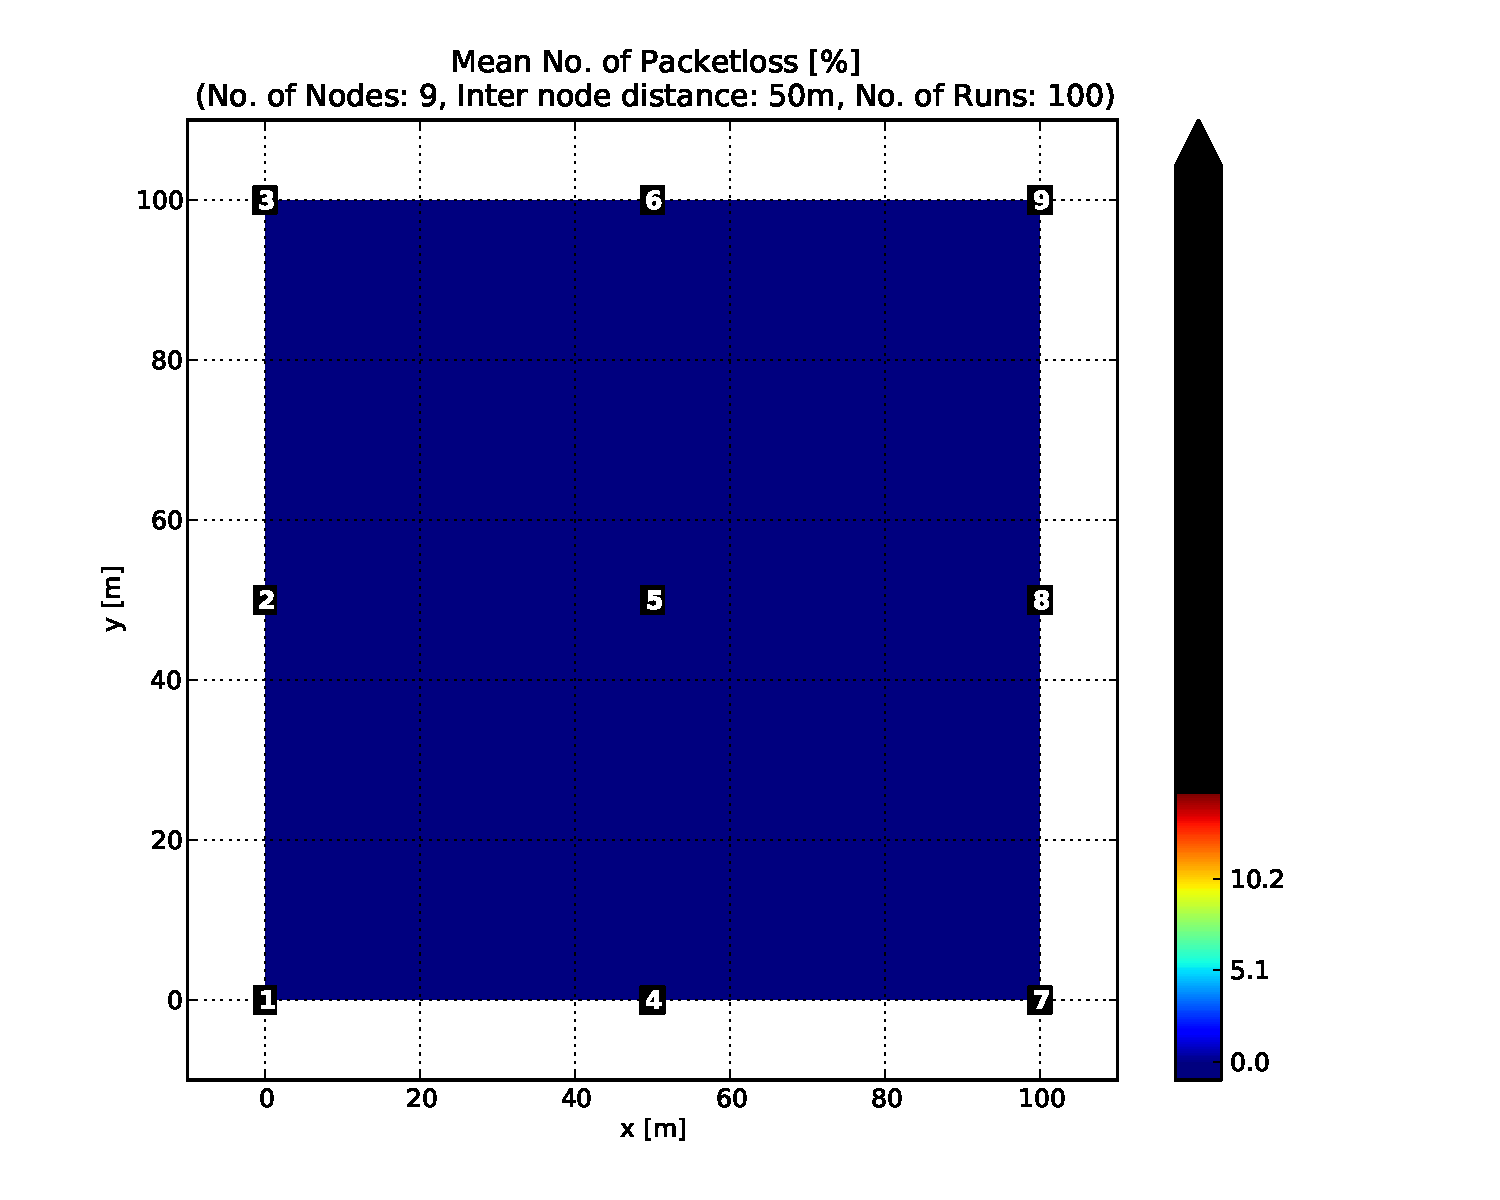
\includegraphics[trim=1.7cm 0cm 3cm 0cm, clip=true, scale=0.38]   {Pics/results/9/OF0/grid/dist50_montecarlo_contour_packetloss.pdf}}
    \subfloat[MRHOF]{\label{fig:9/MRHOF/grid/dist50_montecarlo_contour_packetloss}
      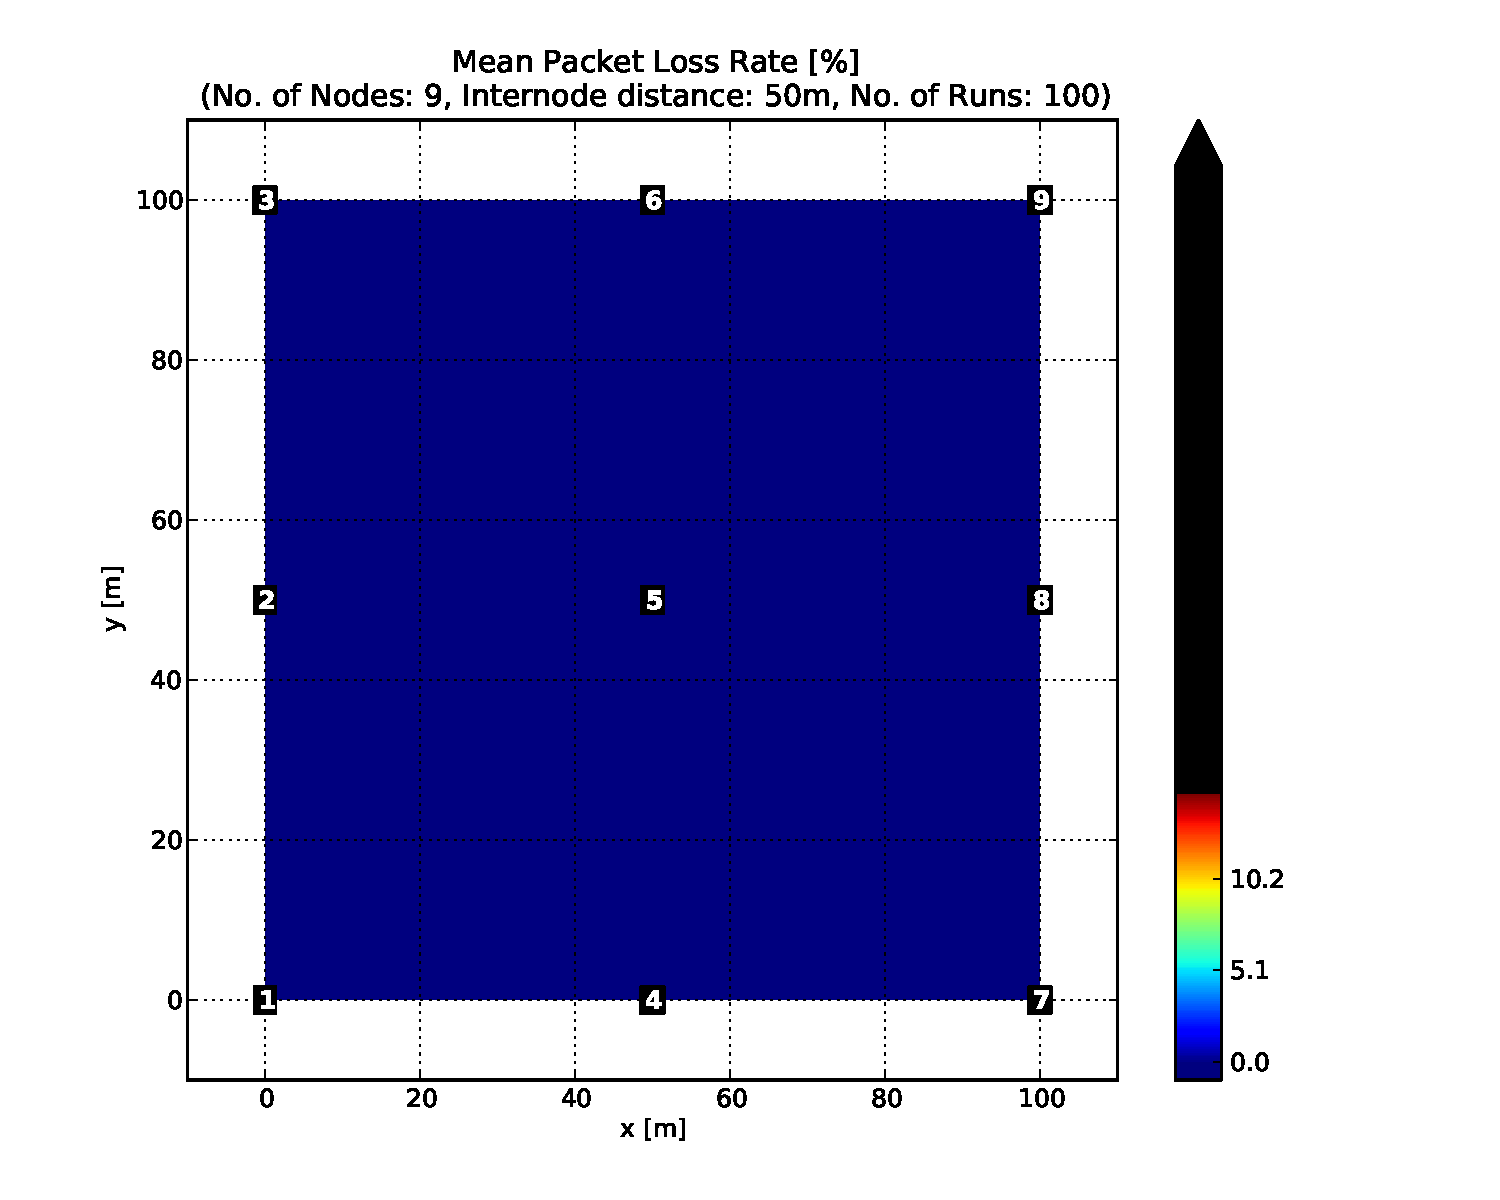
\includegraphics[trim=1.7cm 0cm 3cm 0cm, clip=true, scale=0.38]{Pics/results/9/MRHOF/grid/dist50_montecarlo_contour_packetloss.pdf}}
   \caption{Mean packet loss rate: 9-node grid scenario with 50 m internode distance}
   \label{fig:pl_9_grid_50}
\end{figure}

\begin{figure}[p]
  \centering
    \leavevmode
    \subfloat[OF0]{\label{fig:9/OF0/grid/dist100_montecarlo_contour_packetloss}
     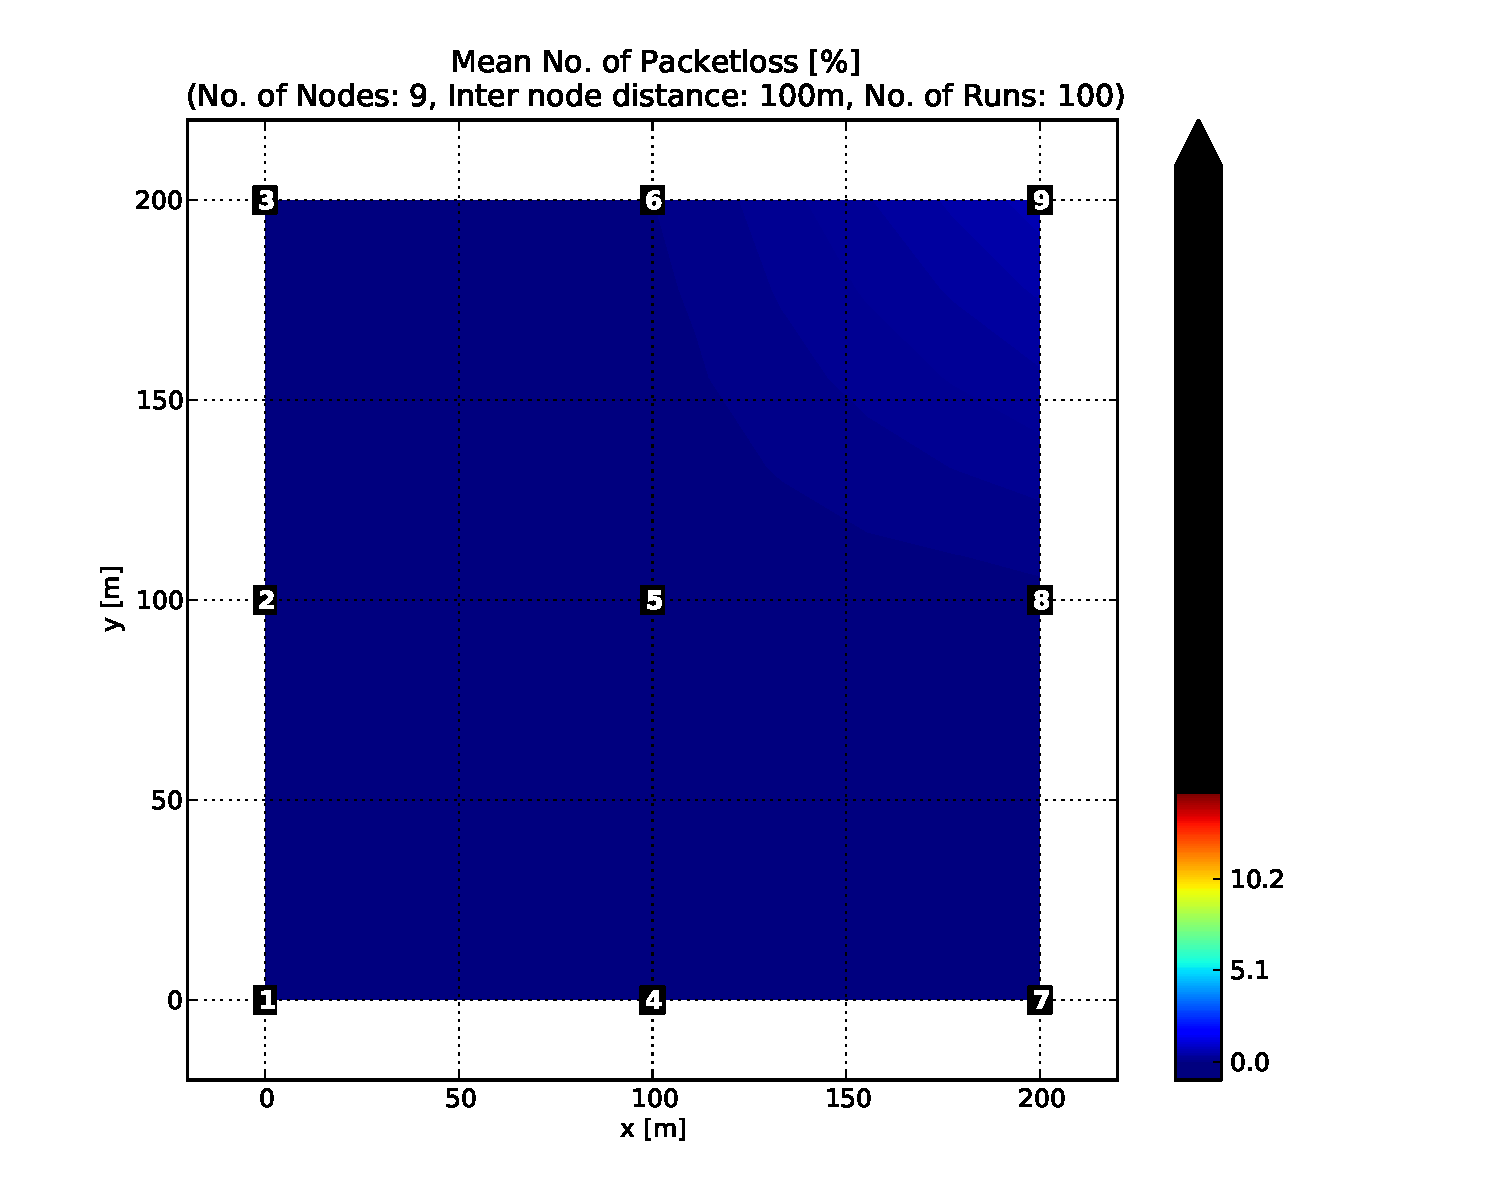
\includegraphics[trim=1.7cm 0cm 3cm 0cm, clip=true, scale=0.38]{Pics/results/9/OF0/grid/dist100_montecarlo_contour_packetloss.pdf}}
    \subfloat[MRHOF]{\label{fig:9/MRHOF/grid/dist100_montecarlo_contour_packetloss}
     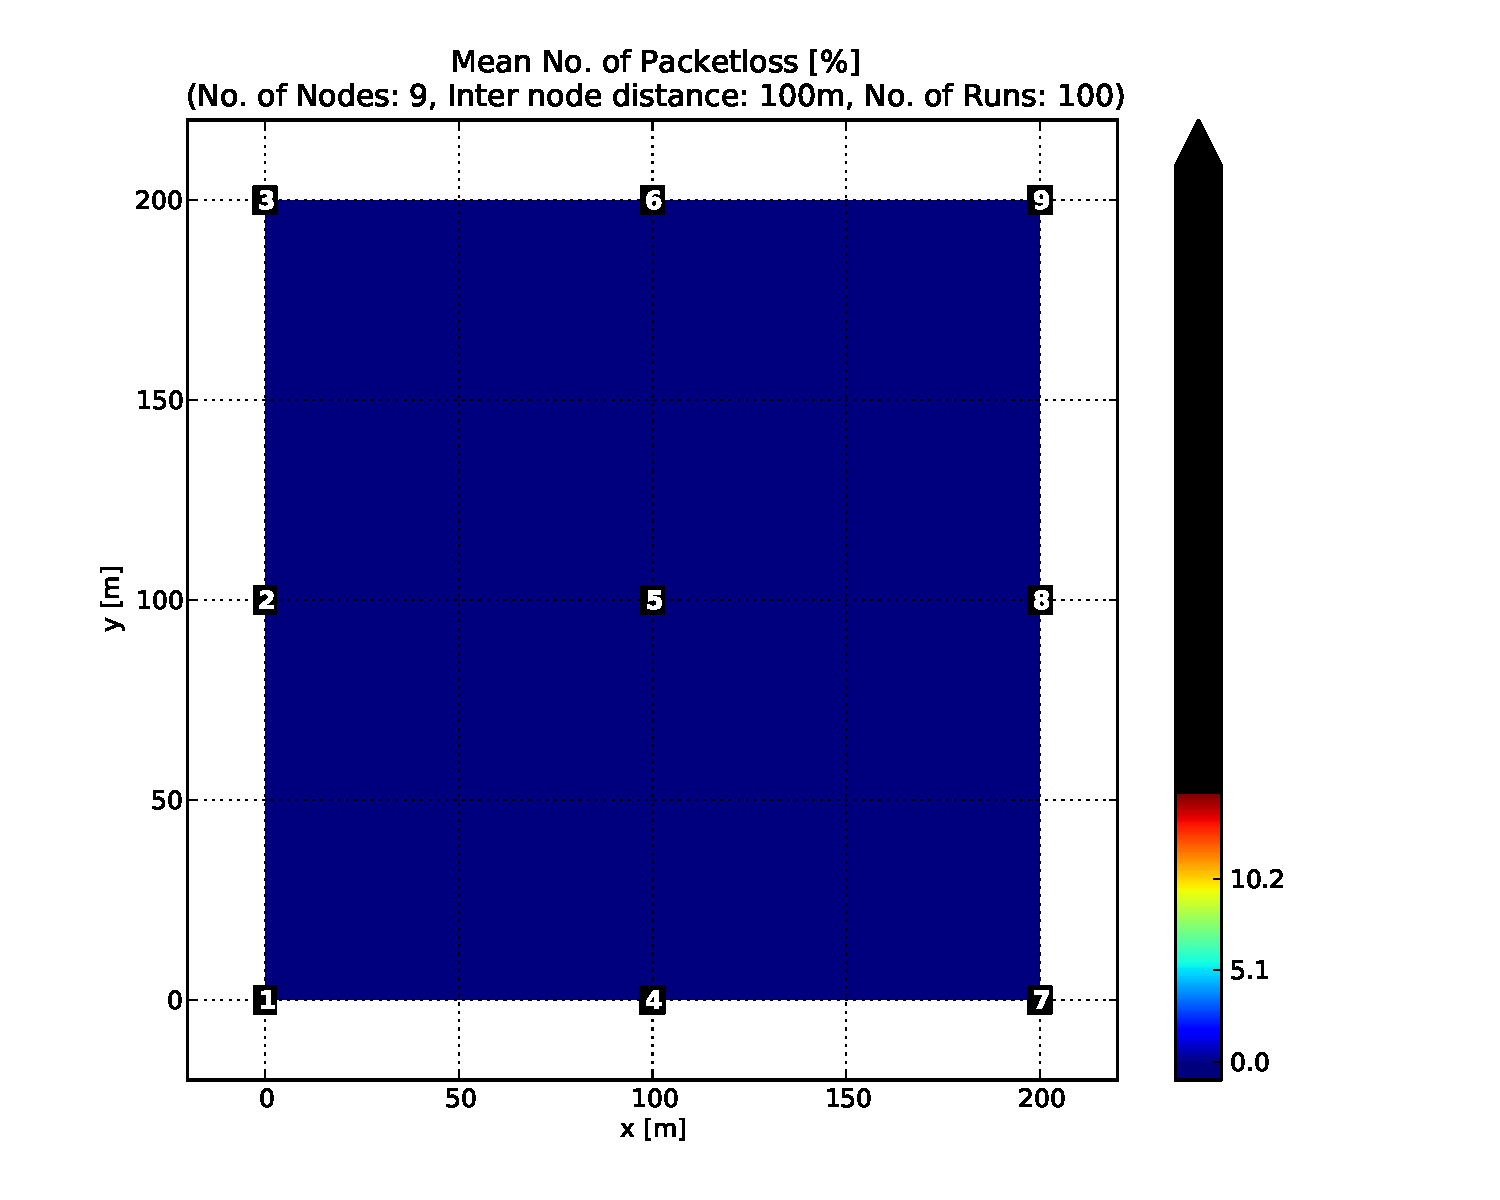
\includegraphics[trim=1.7cm 0cm 3cm 0cm, clip=true, scale=0.38]{Pics/results/9/MRHOF/grid/dist100_montecarlo_contour_packetloss.pdf}}
  \caption{Mean packet loss rate: 9-node grid scenario with 100 m internode distance}
  \label{fig:pl_9_grid_100}
\end{figure}

%%%%%%%%%%%%%%%%%%%%%%%%%%%%%%%%%%%%%%% grid 16 %%%%%%%%%%%%%%%%%%%%%%%%%%%%%%%%%%%%%%%%

\begin{figure}[p]
  \centering
    \leavevmode
    \subfloat[OF0]{\label{fig:16/OF0/grid/dist10_montecarlo_contour_packetloss}
      \includegraphics[trim=1.7cm 0cm 3cm 0cm, clip=true, scale=0.38]{Pics/results/16/OF0/grid/dist10_montecarlo_contour_packetloss.pdf}}
    \subfloat[MRHOF]{\label{fig:16/MRHOF/grid/dist10_montecarlo_contour_packetloss}
      \includegraphics[trim=1.7cm 0cm 3cm 0cm, clip=true, scale=0.38]{Pics/results/16/MRHOF/grid/dist10_montecarlo_contour_packetloss.pdf}}
   \caption{Mean packet loss rate: 16-node grid scenario with 10 m internode distance}
   \label{fig:pl_16_grid_10}
\end{figure}

\begin{figure}[p]
  \centering
    \leavevmode
    \subfloat[OF0]{\label{fig:16/OF0/grid/dist50_montecarlo_contour_packetloss}
    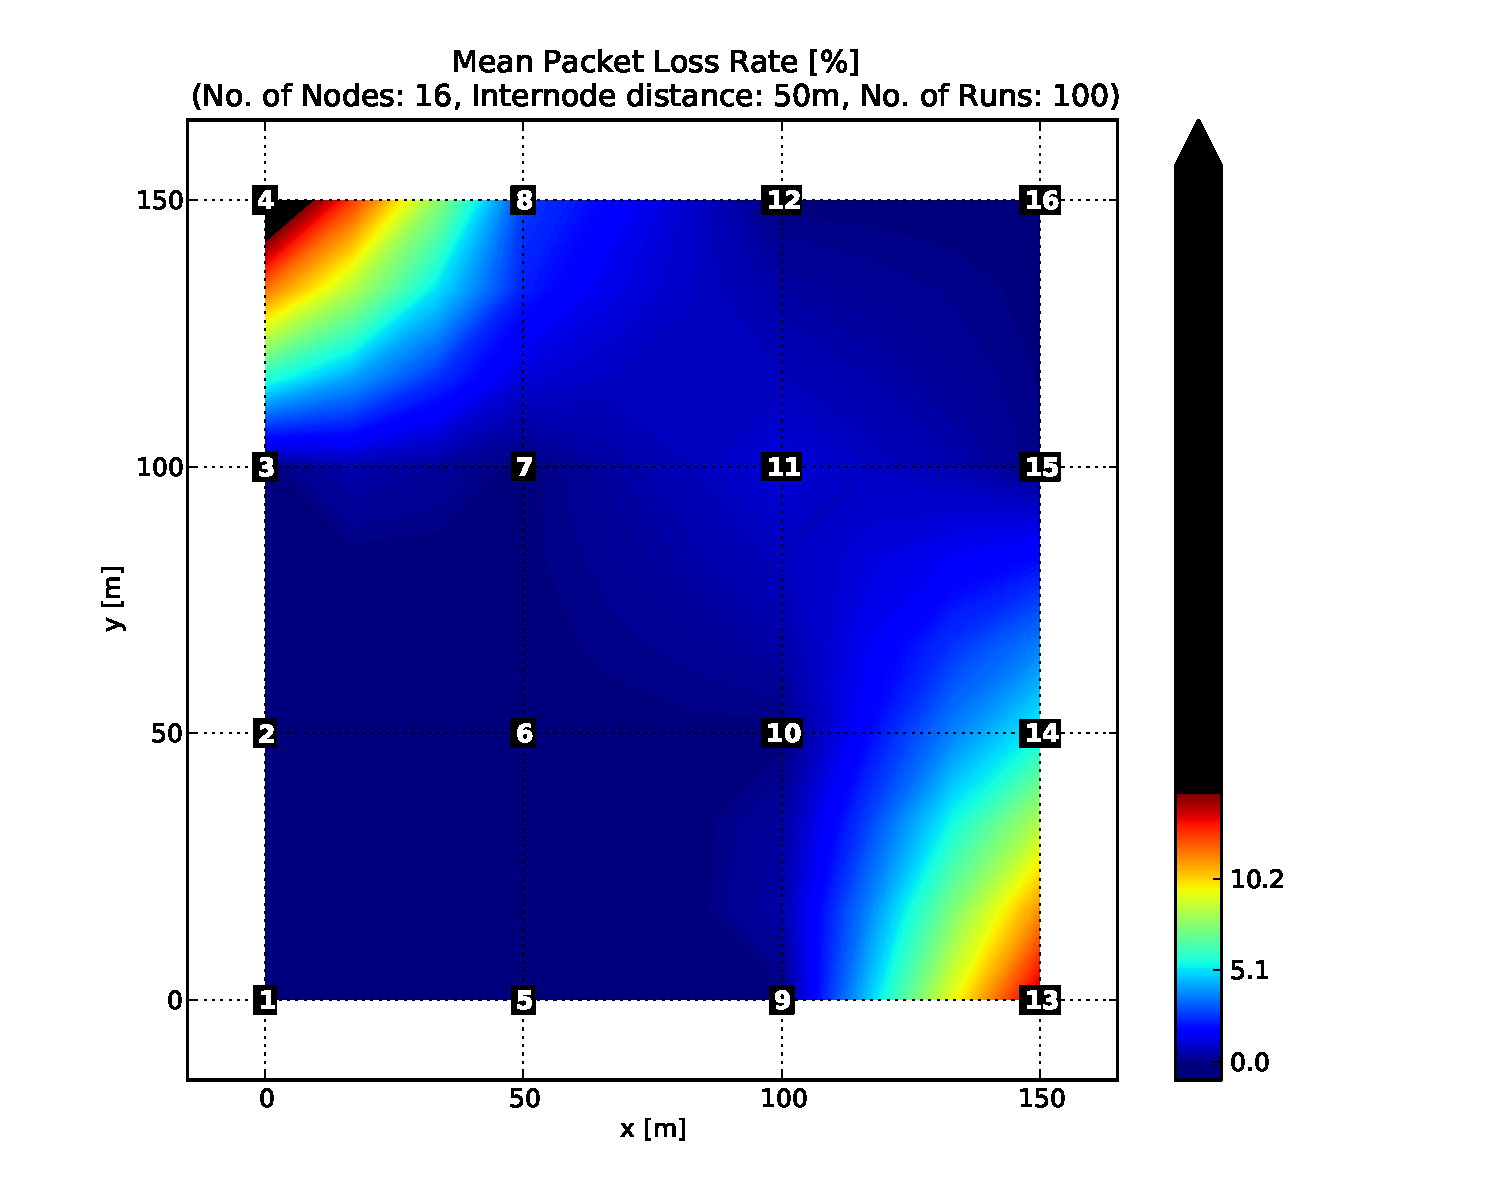
\includegraphics[trim=1.7cm 0cm 3cm 0cm, clip=true, scale=0.38]   {Pics/results/16/OF0/grid/dist50_montecarlo_contour_packetloss.pdf}}
    \subfloat[MRHOF]{\label{fig:16/MRHOF/grid/dist50_montecarlo_contour_packetloss}
      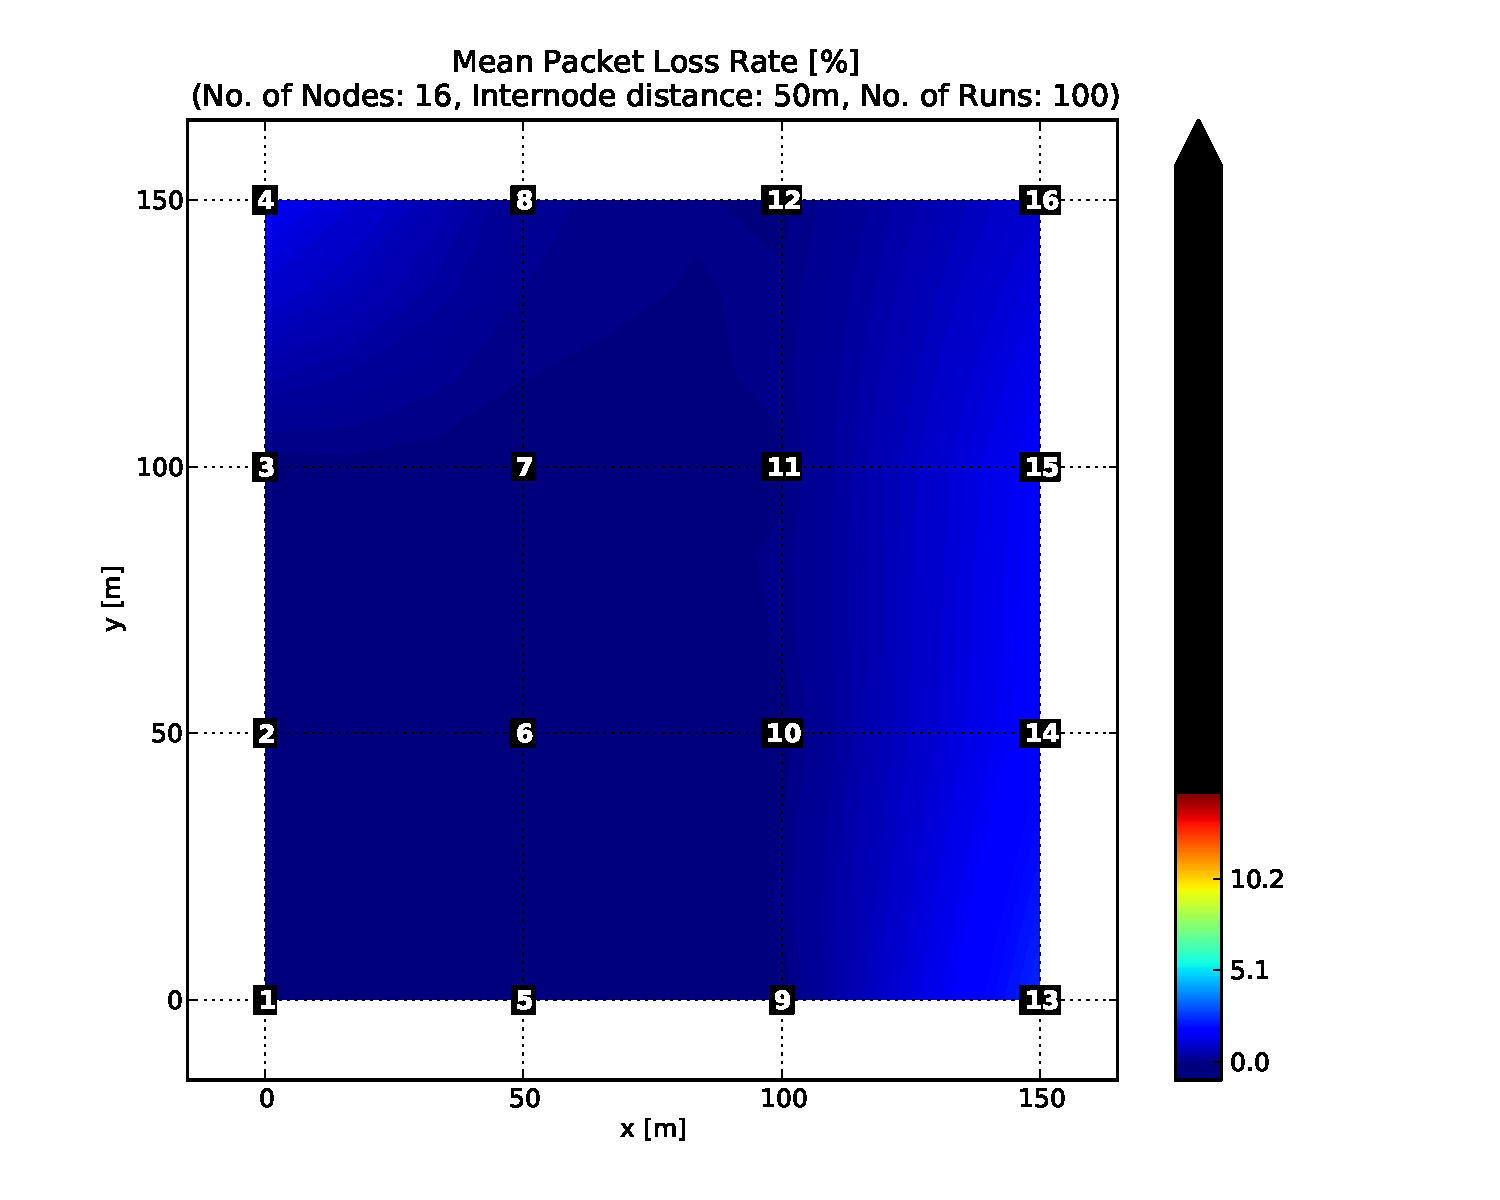
\includegraphics[trim=1.7cm 0cm 3cm 0cm, clip=true, scale=0.38]{Pics/results/16/MRHOF/grid/dist50_montecarlo_contour_packetloss.pdf}}
   \caption{Mean packet loss rate: 16-node grid scenario with 50 m internode distance}
   \label{fig:pl_16_grid_50}
\end{figure}

\begin{figure}[p]
  \centering
    \leavevmode
    \subfloat[OF0]{\label{fig:16/OF0/grid/dist100_montecarlo_contour_packetloss}
     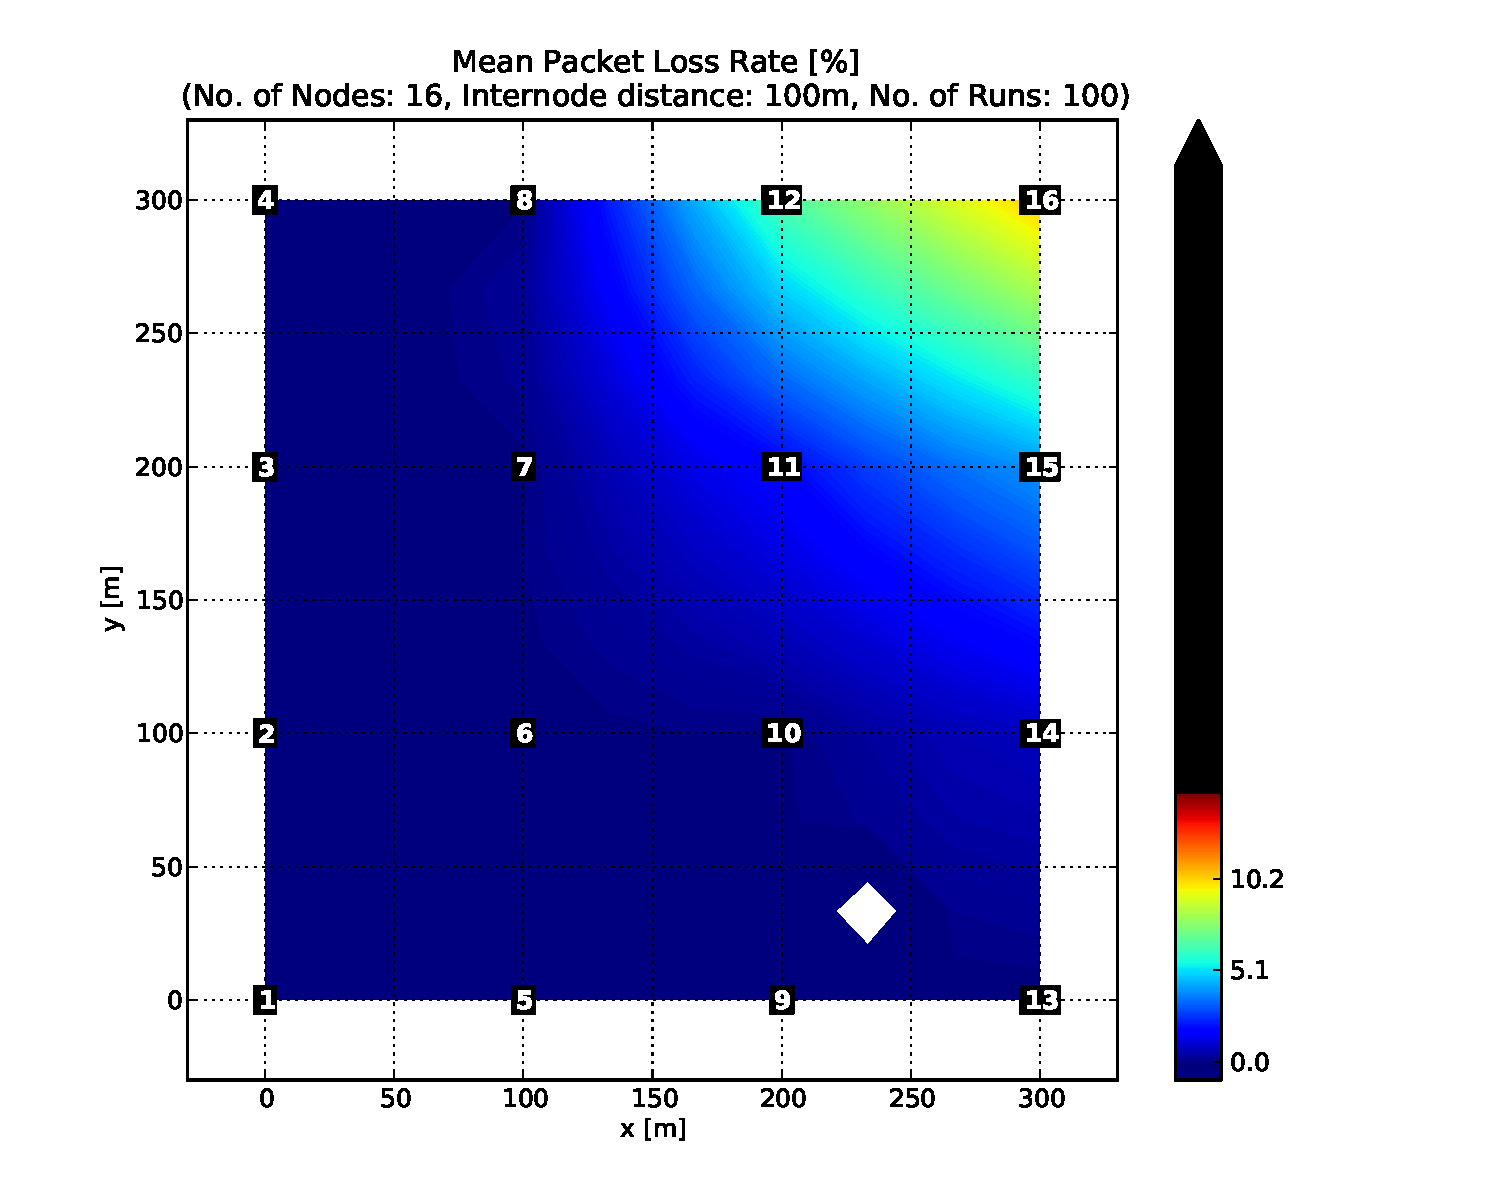
\includegraphics[trim=1.7cm 0cm 3cm 0cm, clip=true, scale=0.38]{Pics/results/16/OF0/grid/dist100_montecarlo_contour_packetloss.pdf}}
    \subfloat[MRHOF]{\label{fig:16/MRHOF/grid/dist100_montecarlo_contour_packetloss}
     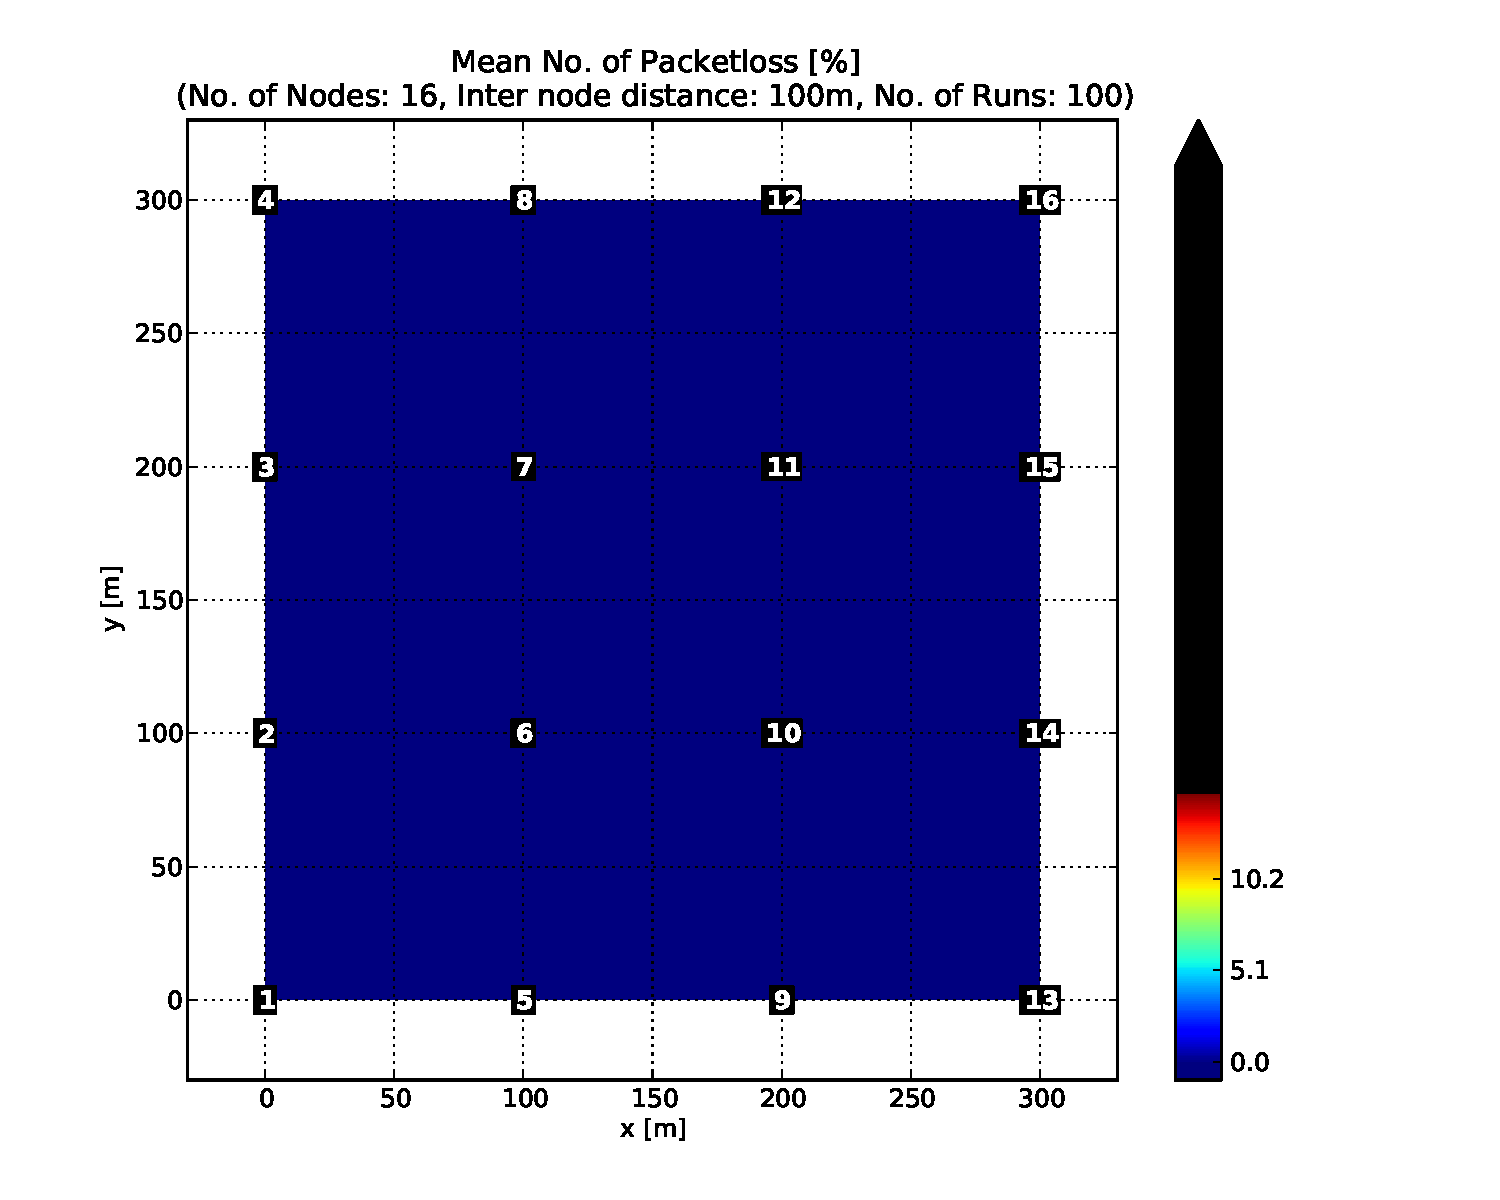
\includegraphics[trim=1.7cm 0cm 3cm 0cm, clip=true, scale=0.38]{Pics/results/16/MRHOF/grid/dist100_montecarlo_contour_packetloss.pdf}}
  \caption{Mean packet loss rate: 16-node grid scenario with 100 m internode distance}
  \label{fig:pl_16_grid_100}
\end{figure}

Compared to the line scenario, the grid scenario is more complicated in terms of routing due to its higher node density and increased route options.  Under this scenario, one can see the packet loss rate goes up with the increase of the internode distance due to the PRR drops. This phenomenon appears more ovbious on the results with OF0 than those with MRHOF, showing that the dropping of PRR has more influence on OF0. Furthermore, OF0 shows a high packet loss in 16-node with 50 meters internode distance (Figure \ref{fig:16/OF0/grid/dist50_montecarlo_contour_packetloss}) while MRHOF gives no more than 5\% packet loss. The packet loss rate of OF0 is also higher than that of MRHOF for 16 nodes with 100 meters internode distance. 
\newline

The packet loss rate comparison between MRHOF and OF0 shows that with OF0 a node is very likely to choose a routing parent with an unreliable link, such as a link with a low PRR; on the other hand, MRHOF with link ETX is more likely to choose a link with the least estimated transmission count, therefore the parent choosing mechanism is more stable and reliable. 

%%%%%%%%%%%%%%%%%%%%%%%%%%%%%%%%%%% RTT %%%%%%%%%%%%%%%%%%%%%%%%%%%%%%%% 
\section{Route Trip Time}
\label{rtt}
 
\subsection{Line Scenario}
\label{line scenario}

The mean RTT for various node numbers and internode distances of line scenario are shown in Figure \ref{fig:rtt_4_line_10} to Figure \ref{fig:rtt_16_line_100}. Agian, the left side figures shows the mean RTT results with OF0, and the right ones shows that with MRHOF.
\newline

Due to the PRR drops as the distance between two nodes increases, the link quality becomes bad, and the packet can not reach the destination within one hop. Therefore RPL forms routes for the multi-hop delivery. This multi-hop delivery can be clearly seen by compareing the results of the 9-node line scenario. When the internode distance is 10 m (Figure \ref{fig:9/OF0/line/dist10_montecarlo_contour}), node 9 is one hop away from the root, and has a mean RTT of 11 ms. When the internode distance increases to 50 m (Figure \ref{fig:9/OF0/line/dist50_montecarlo_contour}), node 9 is at least three hops away from the root, and has a mean RTT of 56 ms. When the internode distance continues to increase to 100 m, node 9 becomes eight hops away, and the mean RTT for node 9 becomes 101 ms. This phenomenon of increasing mean RTT with distance can be observed in the 4- and 16-node scenarios as well. For line scenario, there is no apparent difference between OF0 and MRHOF in terms of increasement of mean RTT ove distance.
\newline

Similar to the Mean packet loss rate results, the mean RTT performances of OF0 and MRHOF are different for the 16-node topology. In Figure \ref{fig:16/OF0/line/dist50_montecarlo_contour} due to the bad routes between the root and the most distant nodes, the mean RTT becomes higher than 250 ms while MRHOF keeps a mean RTT within 150 ms even for the furthest node.
\newline

\begin{figure}[p]
  \centering
    \leavevmode
    \subfloat[OF0]{\label{fig:4/OF0/line/dist10_montecarlo_contour}
      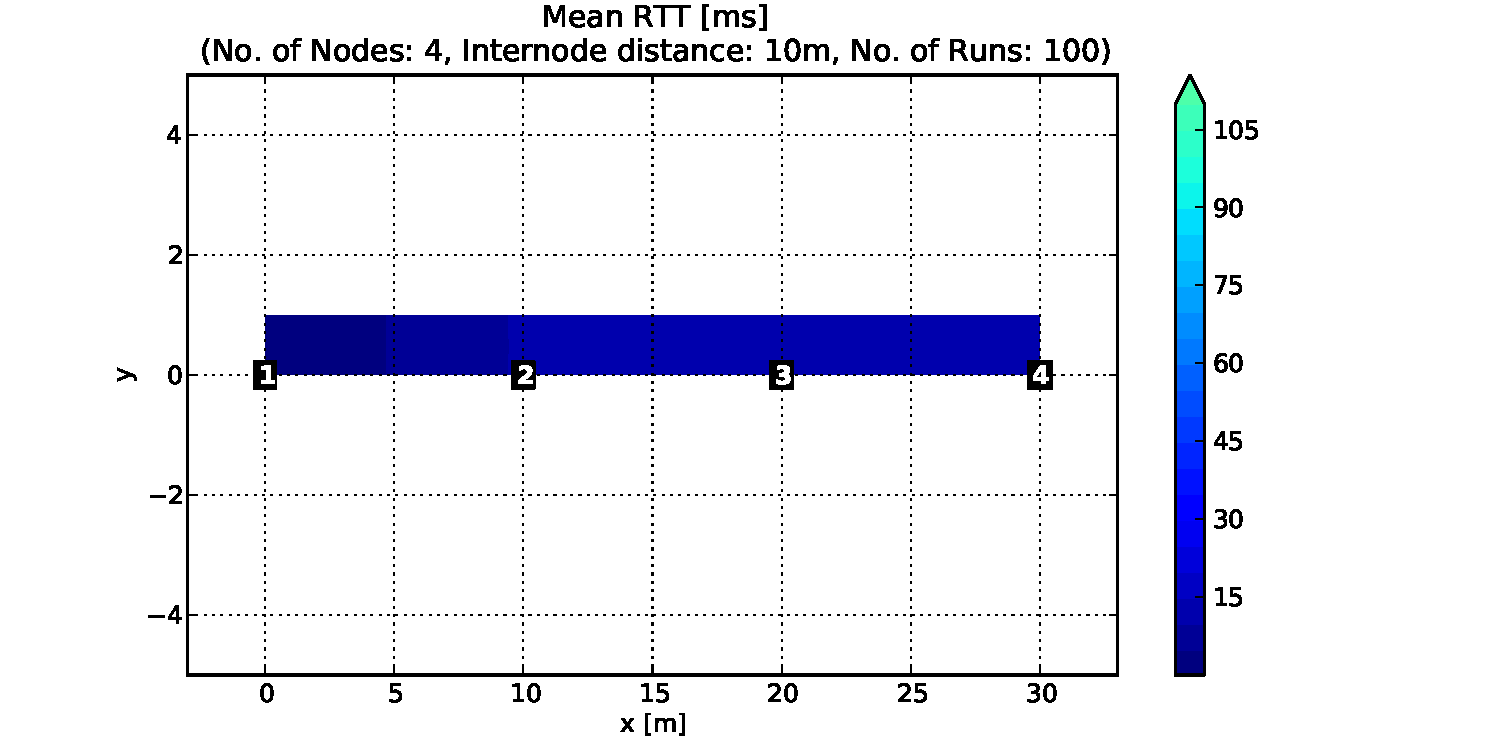
\includegraphics[trim=1.7cm 0cm 3cm 0cm, clip=true, scale=0.38]{Pics/results/4/OF0/line/dist10_montecarlo_contour.pdf}} 
     \subfloat[MRHOF]{\label{fig:4/MRHOF/line/dist10_montecarlo_contour}
      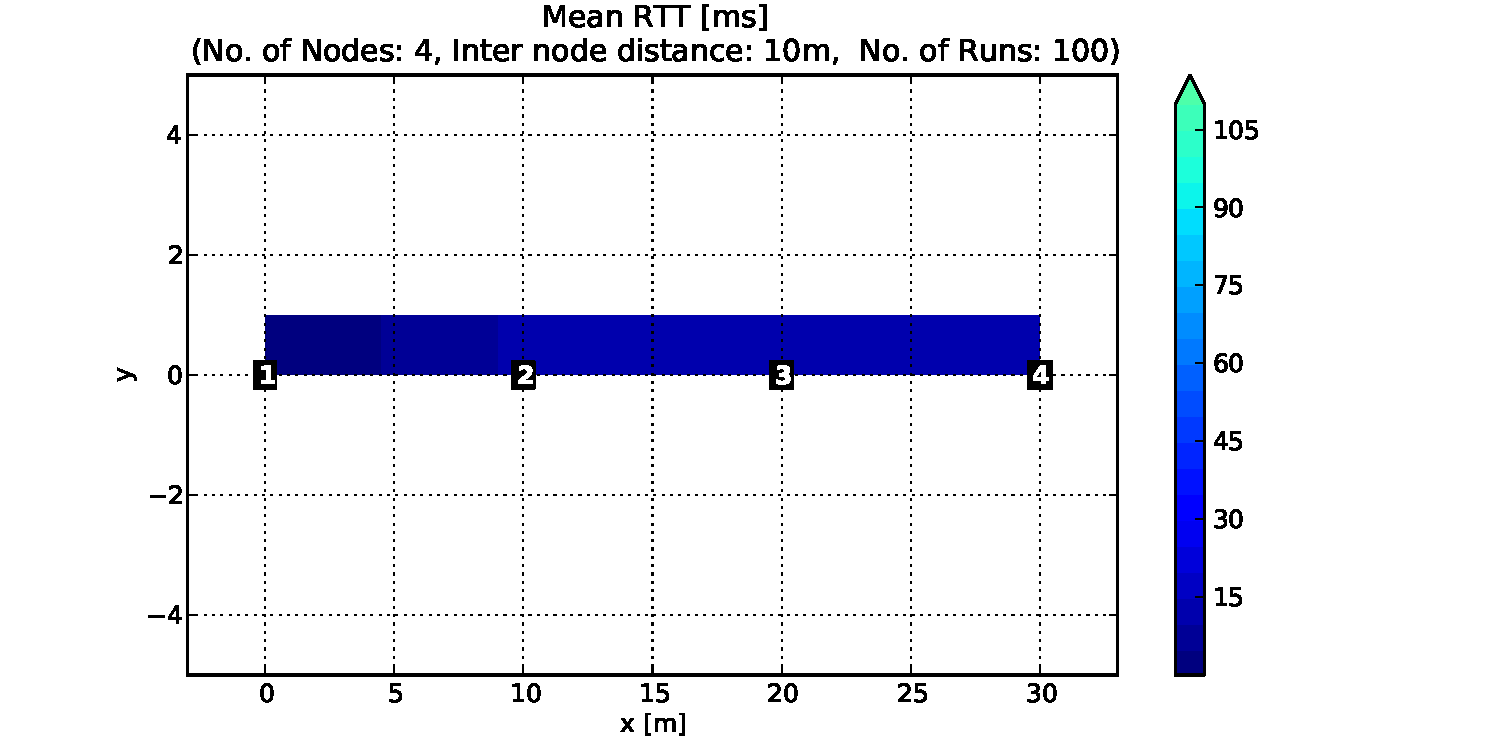
\includegraphics[trim=1.7cm 0cm 3cm 0cm, clip=true, scale=0.38]{Pics/results/4/MRHOF/line/dist10_montecarlo_contour.pdf}}
  \caption{Mean RTT: 4-node line scenario with 10 m internode distance}
 \label{fig:rtt_4_line_10}
\end{figure}

\begin{figure}[p]
  \centering
    \leavevmode
    \subfloat[OF0]{\label{fig:4/OF0/line/dist50_montecarlo_contour}
      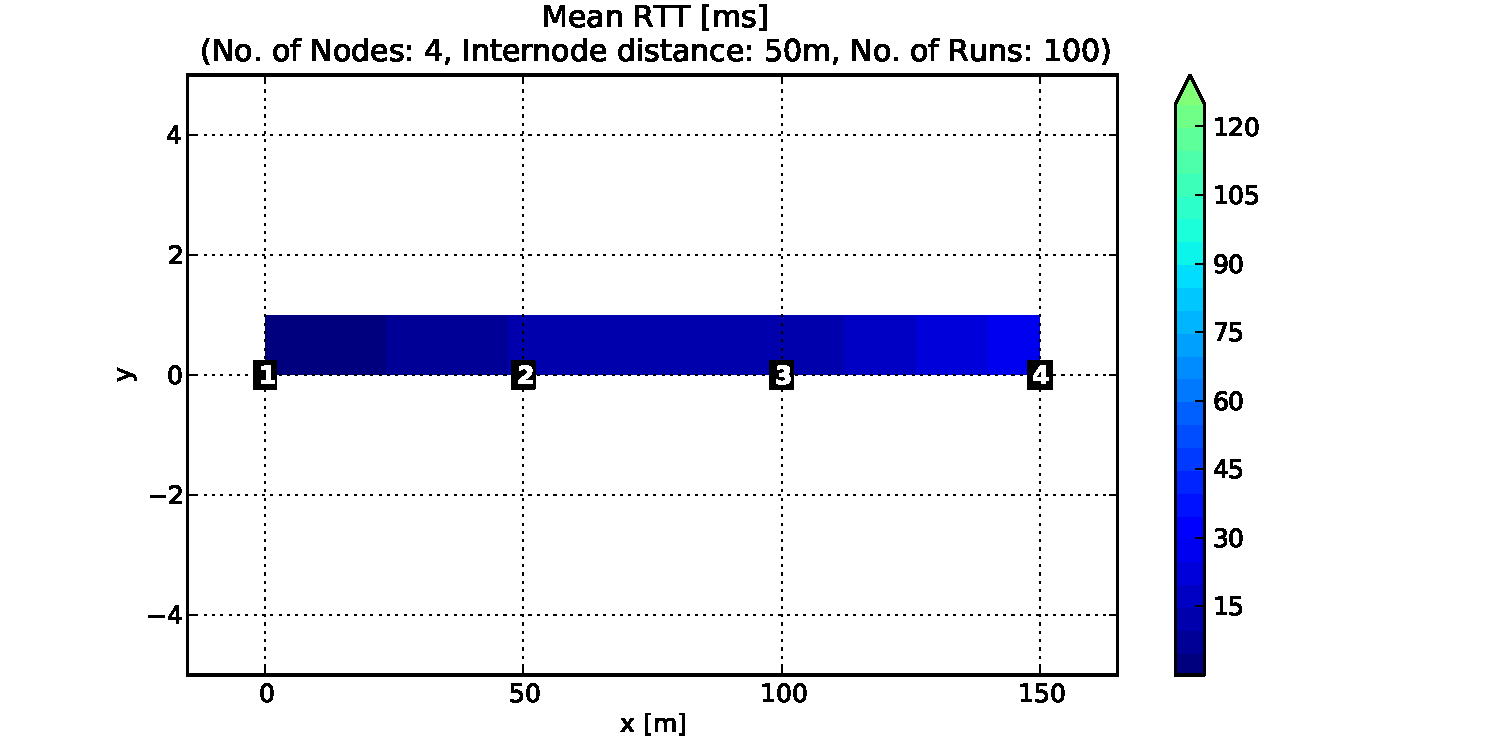
\includegraphics[trim=1.7cm 0cm 3cm 0cm, clip=true, scale=0.38]{Pics/results/4/OF0/line/dist50_montecarlo_contour.pdf}} 
     \subfloat[MRHOF]{\label{fig:4/MRHOF/line/dist50_montecarlo_contour}
      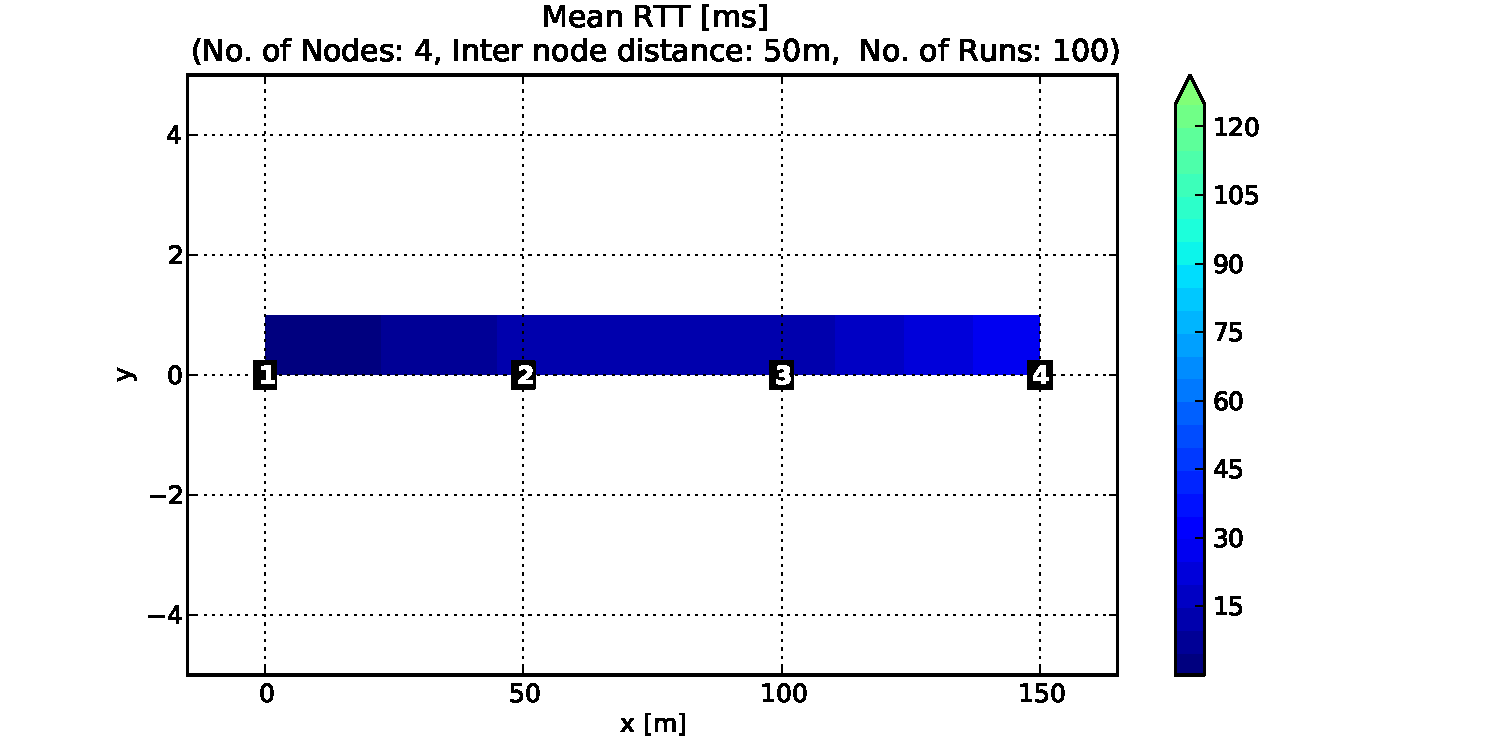
\includegraphics[trim=1.7cm 0cm 3cm 0cm, clip=true, scale=0.38]{Pics/results/4/MRHOF/line/dist50_montecarlo_contour.pdf}}
  \caption{Mean RTT: 4-node line scenario with 50 m internode distance}
 \label{fig:rtt_4_line_50}
\end{figure}

\begin{figure}[p]
  \centering
    \leavevmode
    \subfloat[OF0]{\label{fig:4/OF0/line/dist100_montecarlo_contour}
      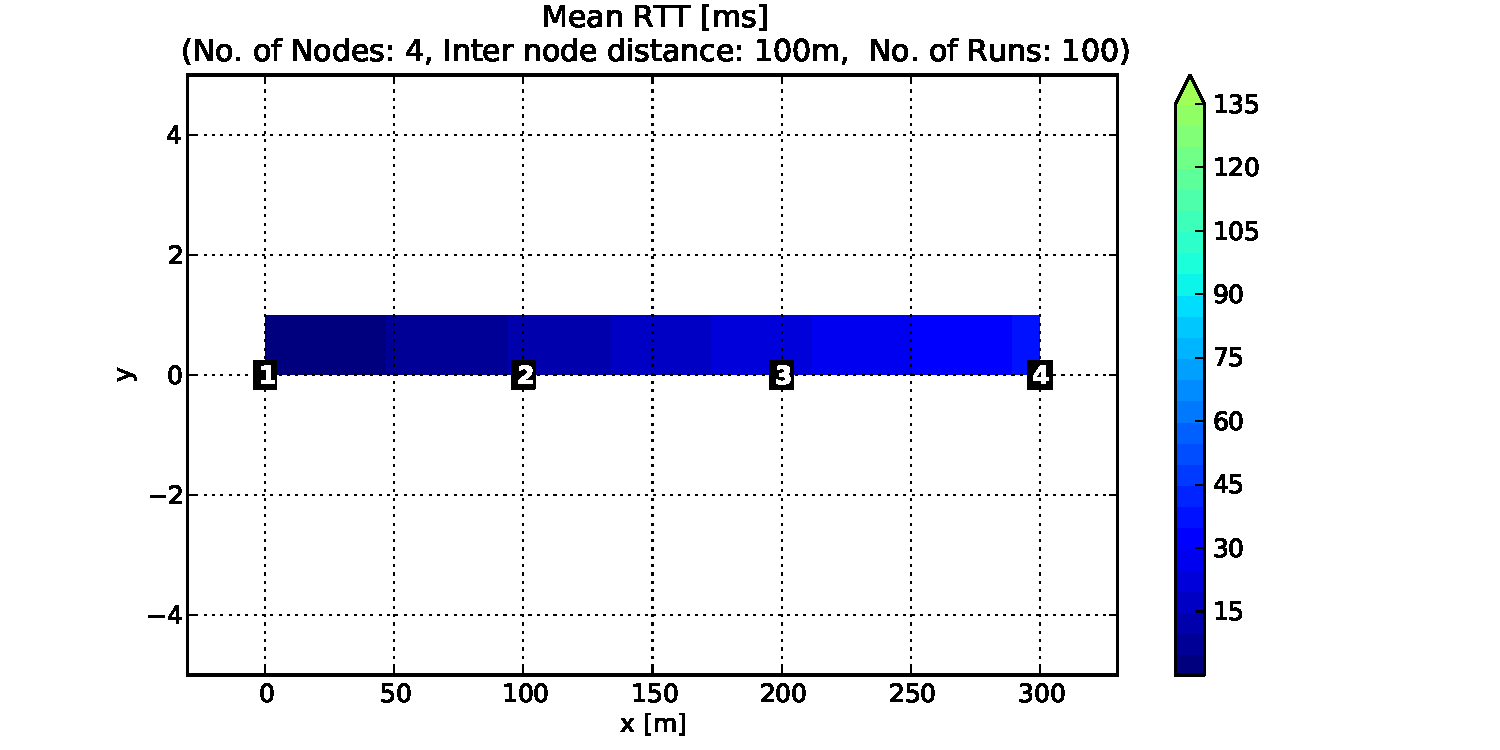
\includegraphics[trim=1.7cm 0cm 3cm 0cm, clip=true, scale=0.38]{Pics/results/4/OF0/line/dist100_montecarlo_contour.pdf}} 
     \subfloat[MRHOF]{\label{fig:4/MRHOF/line/dist100_montecarlo_contour}
      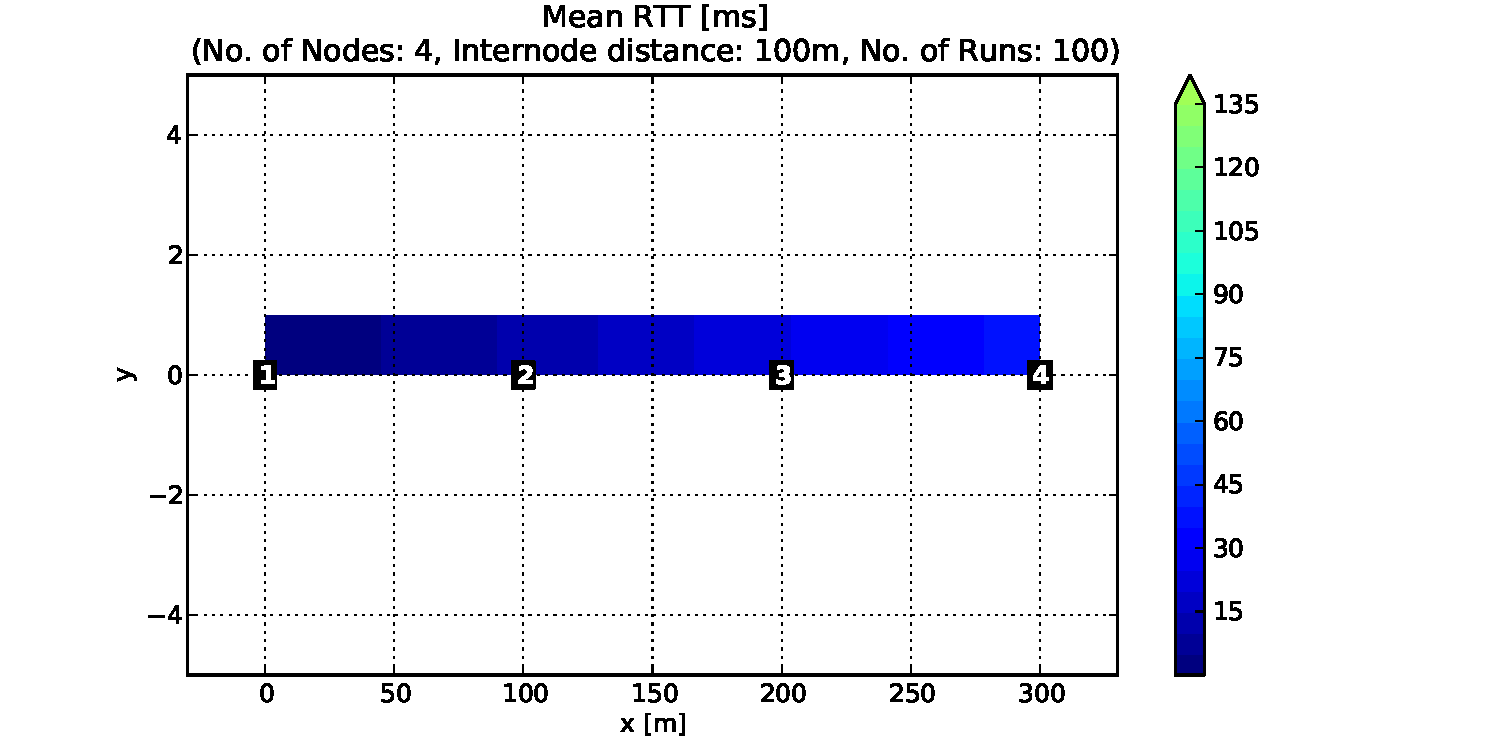
\includegraphics[trim=1.7cm 0cm 3cm 0cm, clip=true, scale=0.38]{Pics/results/4/MRHOF/line/dist100_montecarlo_contour.pdf}}
  \caption{Mean RTT: 4-node line scenario with 100 m internode distance}
 \label{fig:rtt_4_line_100}
\end{figure}

%%%%%%%%%%%%%%%%%%%%%%%%%% line 9 %%%%%%%%%%%%%%%%%%%%%%%%%%%%%%%%%%%%%%%%%%%%%%%%%%%%%%

\begin{figure}[p]
  \centering
    \leavevmode
    \subfloat[OF0]{\label{fig:9/OF0/line/dist10_montecarlo_contour}
      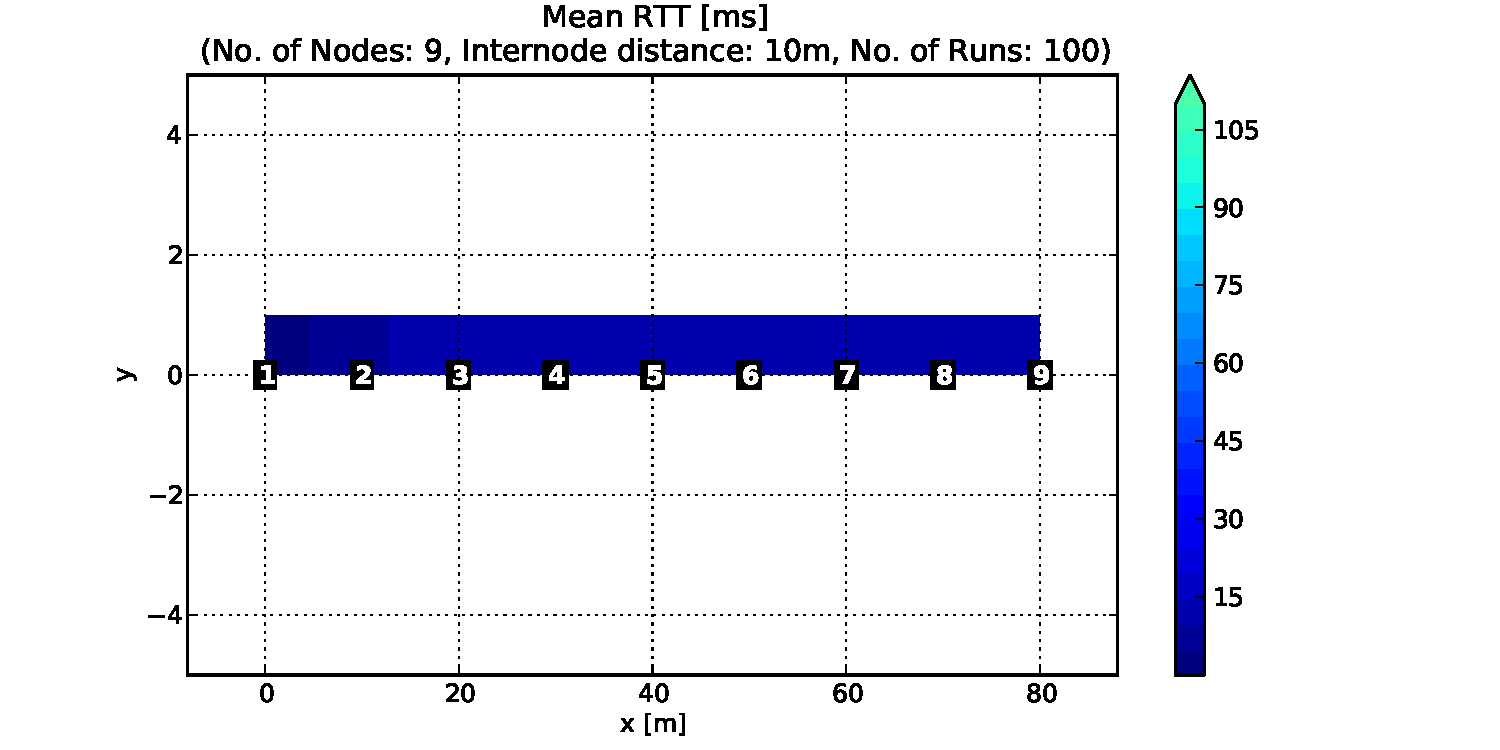
\includegraphics[trim=1.7cm 0cm 3cm 0cm, clip=true, scale=0.38]{Pics/results/9/OF0/line/dist10_montecarlo_contour.pdf}} 
     \subfloat[MRHOF]{\label{fig:9/MRHOF/line/dist10_montecarlo_contour}
      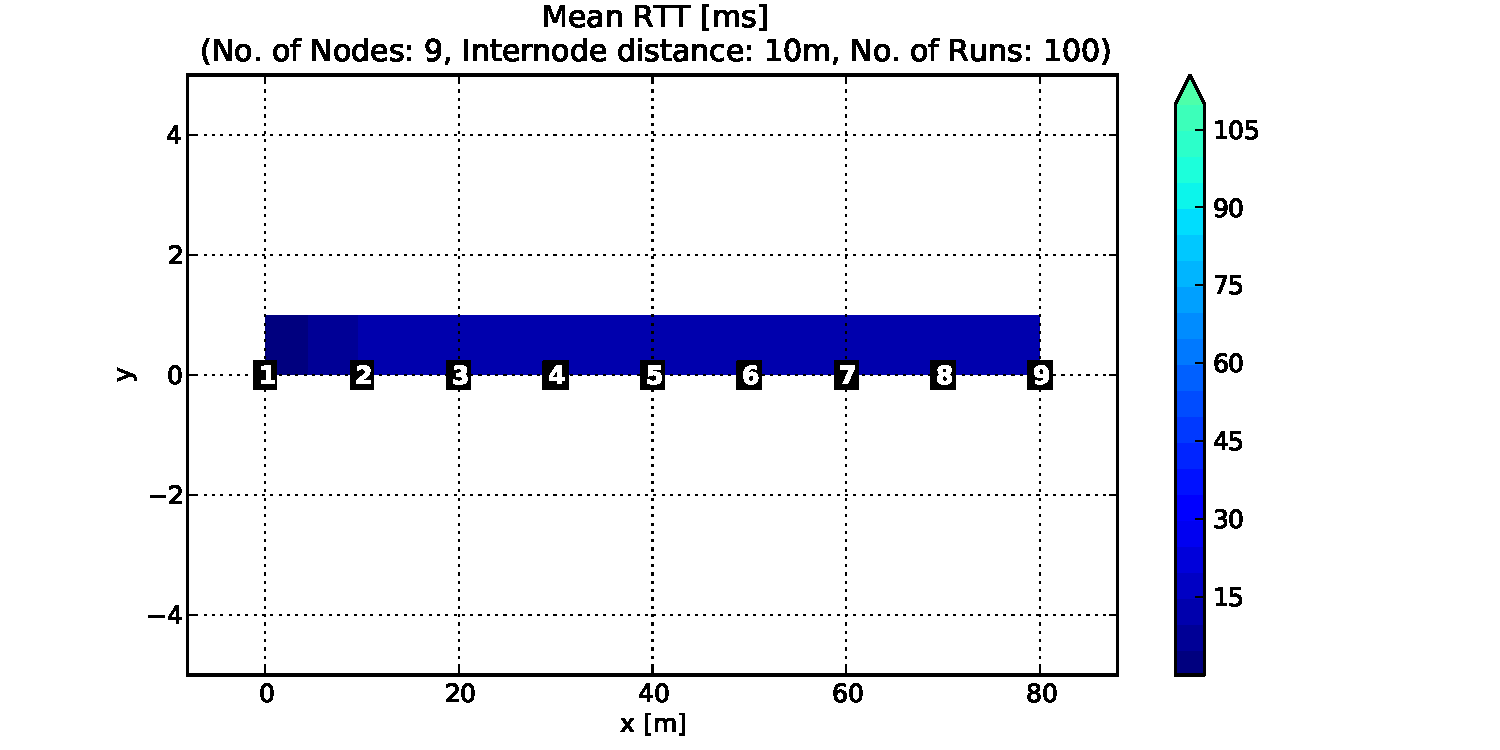
\includegraphics[trim=1.7cm 0cm 3cm 0cm, clip=true, scale=0.38]     {Pics/results/9/MRHOF/line/dist10_montecarlo_contour.pdf}}
  \caption{Mean RTT: 9-node line scenario with 10 m internode distance}
 \label{fig:rtt_9_line_10}
\end{figure}

\begin{figure}[p]
  \centering
    \leavevmode
    \subfloat[OF0]{\label{fig:9/OF0/line/dist50_montecarlo_contour}
      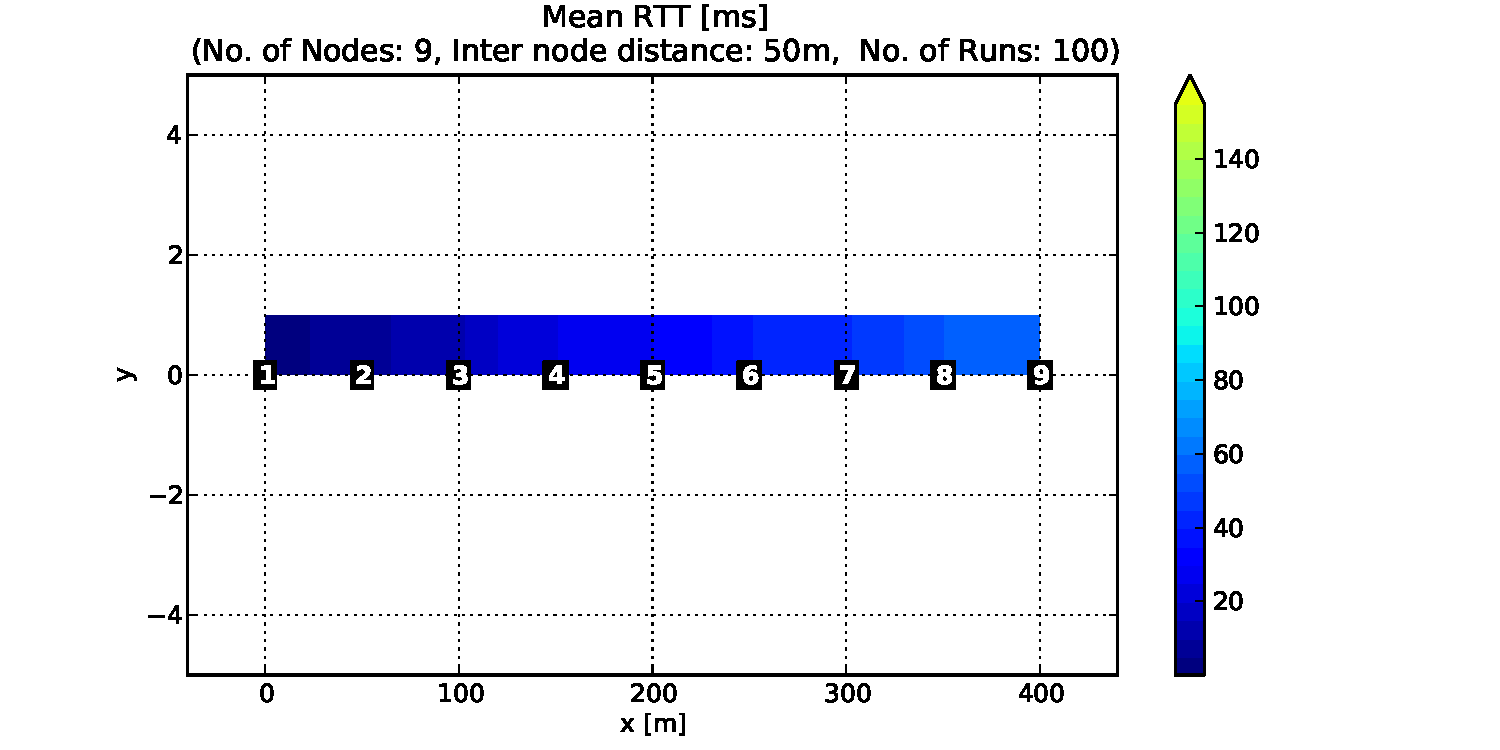
\includegraphics[trim=1.7cm 0cm 3cm 0cm, clip=true, scale=0.38]{Pics/results/9/OF0/line/dist50_montecarlo_contour.pdf}} 
     \subfloat[MRHOF]{\label{fig:9/MRHOF/line/dist50_montecarlo_contour}
      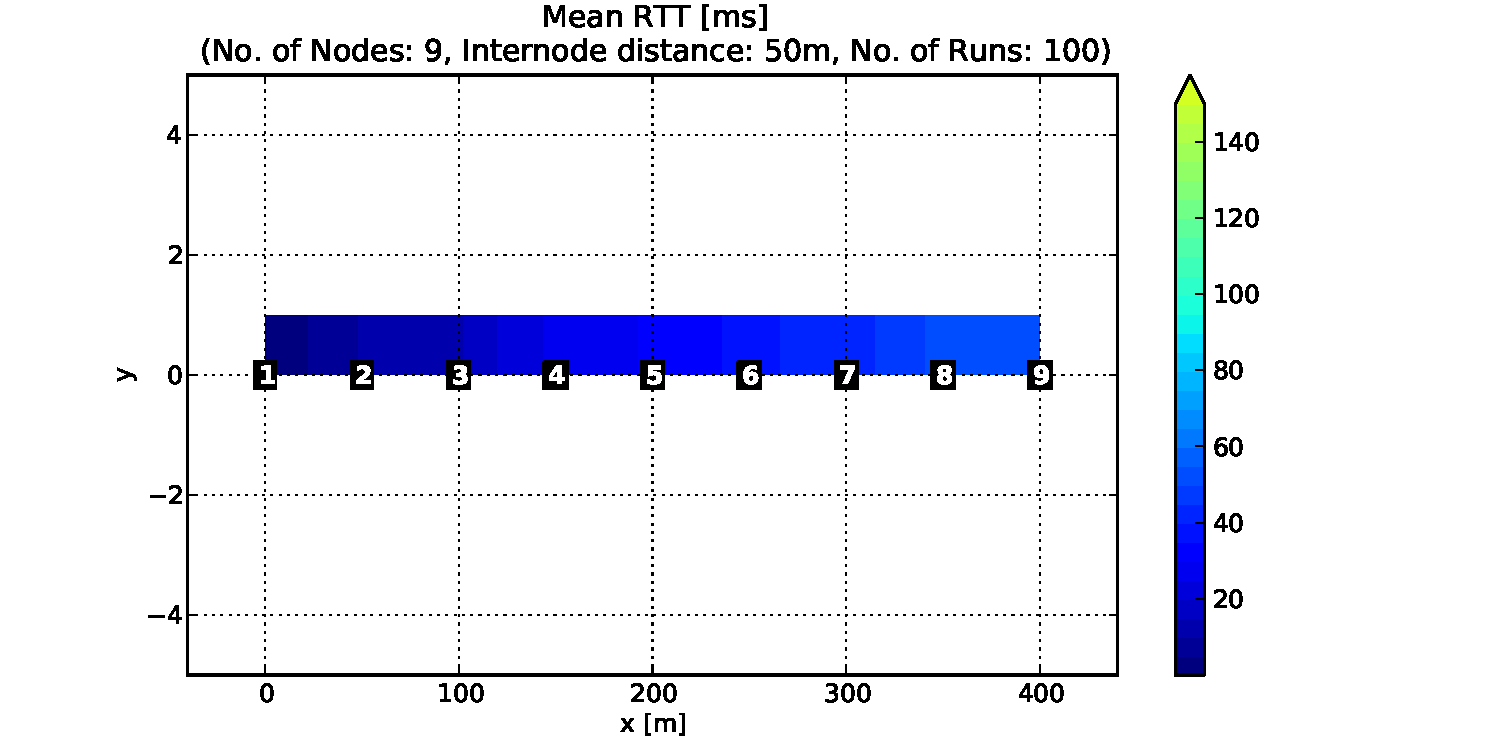
\includegraphics[trim=1.7cm 0cm 3cm 0cm, clip=true, scale=0.38]{Pics/results/9/MRHOF/line/dist50_montecarlo_contour.pdf}}
  \caption{Mean RTT: 9-node line scenario with 50 m internode distance}
 \label{fig:rtt_9_line_50}
\end{figure}

\begin{figure}[p]
  \centering
    \leavevmode
    \subfloat[OF0]{\label{fig:9/OF0/line/dist100_montecarlo_contour}
      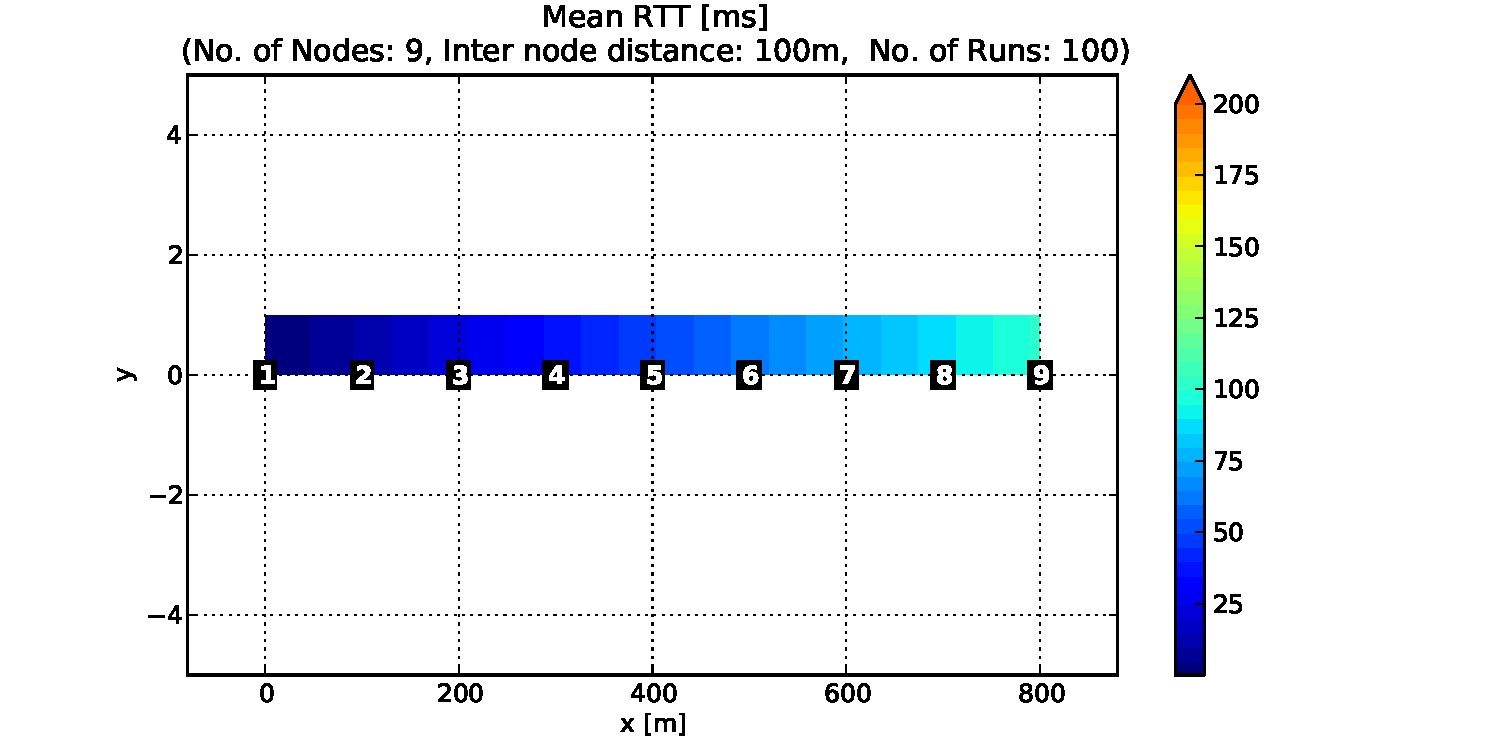
\includegraphics[trim=1.7cm 0cm 3cm 0cm, clip=true, scale=0.38]{Pics/results/9/OF0/line/dist100_montecarlo_contour.pdf}} 
     \subfloat[MRHOF]{\label{fig:9/MRHOF/line/dist100_montecarlo_contour}
      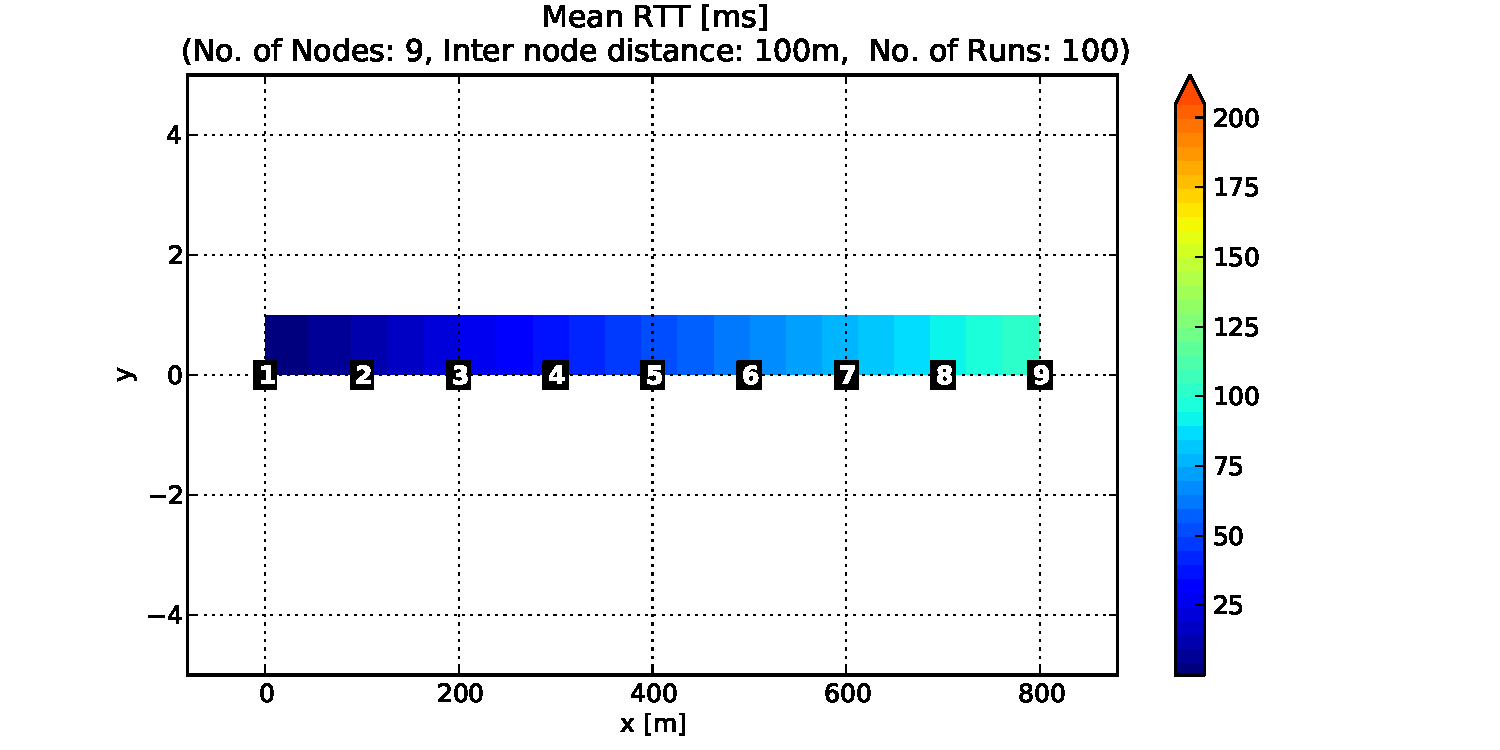
\includegraphics[trim=1.7cm 0cm 3cm 0cm, clip=true, scale=0.38]{Pics/results/9/MRHOF/line/dist100_montecarlo_contour.pdf}}
  \caption{Mean RTT: 9-node line scenario with 100 m internode distance}
 \label{fig:rtt__line_100}
\end{figure}

%%%%%%%%%%%%%%%%%%%%%%%%%%%%%%%%%% line 16 %%%%%%%%%%%%%%%%%%%%%%%%%%%%%%%%%%%%%%

\begin{figure}[p]
  \centering
    \leavevmode
    \subfloat[OF0]{\label{fig:16/OF0/line/dist10_montecarlo_contour}
      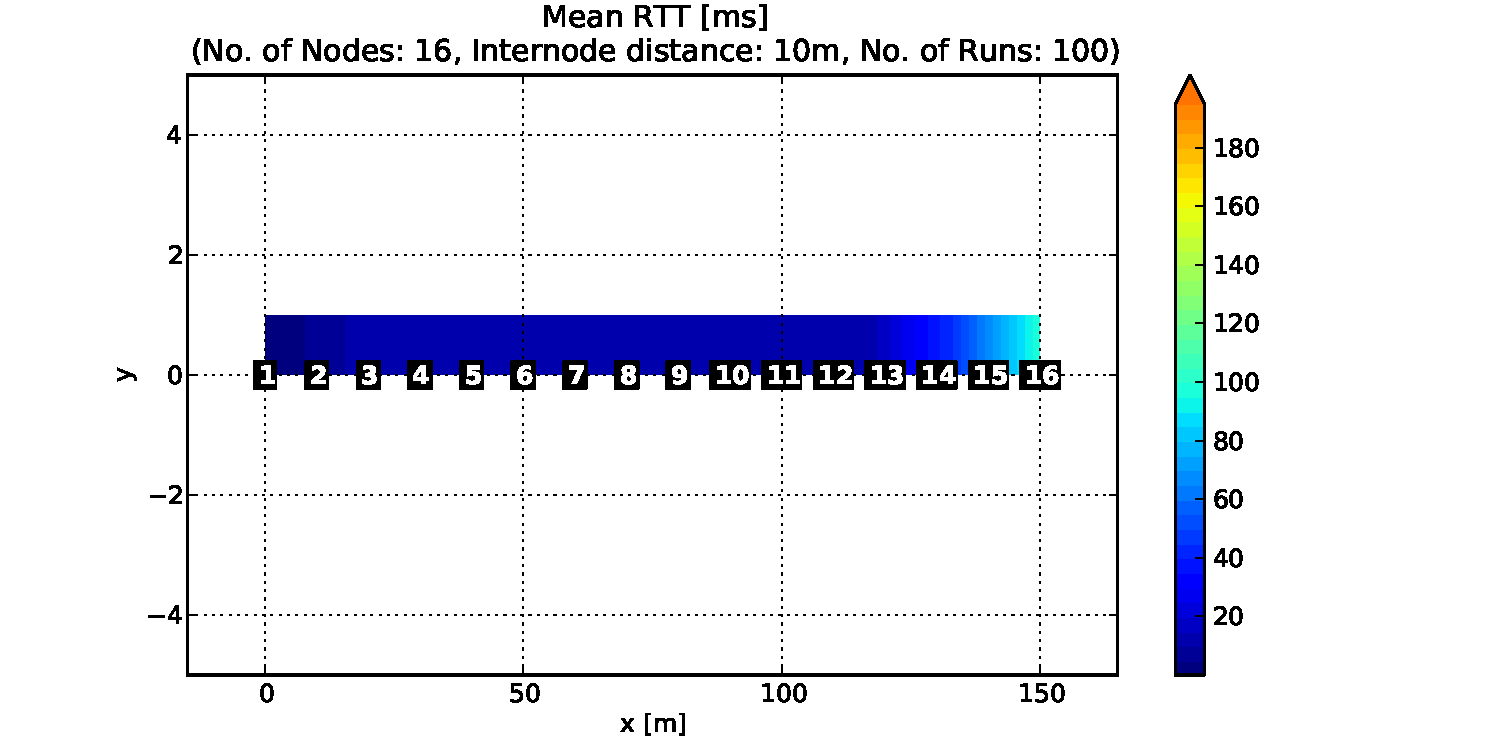
\includegraphics[trim=1.7cm 0cm 3cm 0cm, clip=true, scale=0.38]{Pics/results/16/OF0/line/dist10_montecarlo_contour.pdf}} 
     \subfloat[MRHOF]{\label{fig:16/MRHOF/line/dist10_montecarlo_contour}
      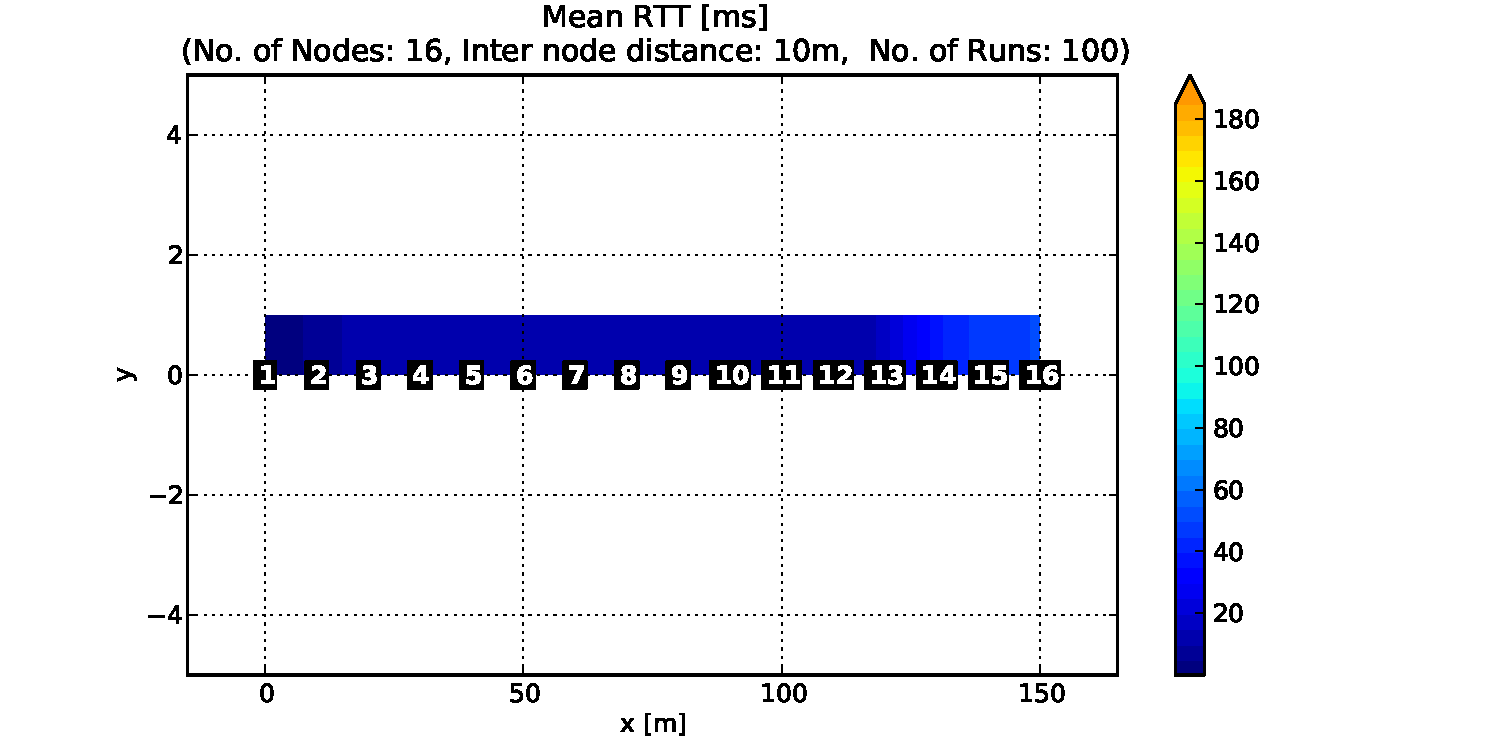
\includegraphics[trim=1.7cm 0cm 3cm 0cm, clip=true, scale=0.38]{Pics/results/16/MRHOF/line/dist10_montecarlo_contour.pdf}}
  \caption{Mean RTT: 16-node line scenario with 10 m internode distance}
 \label{fig:rtt_16_line_10}
\end{figure}

\begin{figure}[p]
  \centering
    \leavevmode
    \subfloat[OF0]{\label{fig:16/OF0/line/dist50_montecarlo_contour}
      \includegraphics[trim=1.7cm 0cm 3cm 0cm, clip=true, scale=0.38]{Pics/results/16/OF0/line/dist50_montecarlo_contour.pdf}} 
     \subfloat[MRHOF]{\label{fig:16/MRHOF/line/dist50_montecarlo_contour}
      \includegraphics[trim=1.7cm 0cm 3cm 0cm, clip=true, scale=0.38]{Pics/results/16/MRHOF/line/dist50_montecarlo_contour.pdf}}
  \caption{Mean RTT: 16-node line scenario with 50 m internode distance}
 \label{fig:rtt_16_line_50}
\end{figure}

\begin{figure}[p]
  \centering
    \leavevmode
    \subfloat[OF0]{\label{fig:16/OF0/line/dist100_montecarlo_contour}
      \includegraphics[trim=1.7cm 0cm 3cm 0cm, clip=true, scale=0.38] {Pics/results/16/OF0/line/dist100_montecarlo_contour.pdf}} 
     \subfloat[MRHOF]{\label{fig:16/MRHOF/line/dist100_montecarlo_contour}
      \includegraphics[trim=1.7cm 0cm 3cm 0cm, clip=true, scale=0.38]{Pics/results/16/MRHOF/line/dist100_montecarlo_contour.pdf}}
  \caption{Mean RTT: 16-node line scenario with 100 m internode distance}
 \label{fig:rtt_16_line_100}
\end{figure}

\subsection{Grid Scenario}
\label{rtt:grid}

Figure \ref{fig:rtt_4_grid_10} to Figure \ref{fig:rtt_16_grid_100} illustrate the mean RTT results of the grid scenario simulations.
\newline

The phenomenon of increasing mean RTT with internode distance (mentioned in Section \ref{rtt:line}) can be observed here again. In Figure \ref{fig:4/OF0/grid/dist50_montecarlo_contour} and Figure \ref{fig:4/OF0/grid/dist100_montecarlo_contour}, one can see the mean RTT increasement with distance of a 4-node grid scenario using OF0 as routing OF. The mean RTT for node 4 increases from  10.7 ms to 73.8 ms while the internode distance increases from 50 m to 100 m. Similaly, in Figure \ref{fig:4/MRHOF/grid/dist50_montecarlo_contour} and Figure \ref{fig:4/MRHOF/grid/dist100_montecarlo_contour}, by using MRHOF the mean RTT for node 4 increases from  11.1 ms to 69.4 ms while the internode distance increases from 50 m to 100 m.
\newline

When the node number increases, the difference between OF0 and MRHOF in terms of mean RTT increasement over distance grows bigger. For the 9-node grid scenario with OF0, the mean RTT of node 9 increases from 72.5 ms (internode distance 50 m, Figure \ref{fig:9/OF0/grid/dist50_montecarlo_contour}) to 142.1 ms (internode distance 100 m, Figure \ref{fig:9/OF0/grid/dist100_montecarlo_contour}) while with MRHOF it increases from 68.2 ms (internode distance 50 m, Figure \ref{fig:9/MRHOF/grid/dist50_montecarlo_contour}) to 79.9 ms (internode distance 100 m, Figure \ref{fig:9/MRHOF/grid/dist100_montecarlo_contour}. For the 16-node grid scenario using OF0, the mean RTT of node 16 increases from 35.1 ms (internode distance 50 m, Figure \ref{fig:16/OF0/grid/dist50_montecarlo_contour}) to infinite (internode distance 100 m, Figure \ref{fig:9/OF0/grid/dist100_montecarlo_contour}) due to broken route between the root and node 16 in one or more runs. On the other hand, with MRHOF node 16 has a mean RTT growth from 50.8 ms (internode distance 50 m, Figure \ref{fig:16/MRHOF/grid/dist50_montecarlo_contour}) to 116.0 ms (internode distance 100 m, Figure \ref{fig:16/MRHOF/grid/dist100_montecarlo_contour}).
\newline

Moreover, in Figure \ref{fig:16/OF0/grid/dist50_montecarlo_contour} and Figure \ref{fig:16/OF0/grid/dist100_montecarlo_contour}, one can see when using OF0, there are some more instances of broken routes between the root and the nodes with the infinite mean RTT values. 
\newline

By comparing the mean RTT results of OF0 and MRHOF, one can say that in terms of mean RTT MRHOF most likely to perform better than OF0 for the nodes which are more than one hop away. 
\newline

\begin{figure}[p]
  \centering
    \leavevmode
    \subfloat[OF0]{\label{fig:4/OF0/grid/dist10_montecarlo_contour}
      \includegraphics[trim=1.7cm 0cm 3cm 0cm, clip=true, scale=0.38]{Pics/results/4/OF0/grid/dist10_montecarlo_contour.pdf}} 
     \subfloat[MRHOF]{\label{fig:4/MRHOF/grid/dist10_montecarlo_contour}
      \includegraphics[trim=1.7cm 0cm 3cm 0cm, clip=true, scale=0.38]{Pics/results/4/MRHOF/grid/dist10_montecarlo_contour.pdf}}
  \caption{Mean RTT: 4-node grid scenario with 10 m internode distance}
 \label{fig:rtt_4_grid_10}
\end{figure}

\begin{figure}[p]
  \centering
    \leavevmode
    \subfloat[OF0]{\label{fig:4/OF0/grid/dist50_montecarlo_contour}
      \includegraphics[trim=1.7cm 0cm 3cm 0cm, clip=true, scale=0.38]{Pics/results/4/OF0/grid/dist50_montecarlo_contour.pdf}} 
     \subfloat[MRHOF]{\label{fig:4/MRHOF/grid/dist50_montecarlo_contour}
      \includegraphics[trim=1.7cm 0cm 3cm 0cm, clip=true, scale=0.38]{Pics/results/4/MRHOF/grid/dist50_montecarlo_contour.pdf}}
  \caption{Mean RTT: 4-node grid scenario with 50 m internode distance}
 \label{fig:rtt_4_grid_50}
\end{figure}

\begin{figure}[p]
  \centering
    \leavevmode
    \subfloat[OF0]{\label{fig:4/OF0/grid/dist100_montecarlo_contour}
      \includegraphics[trim=1.7cm 0cm 3cm 0cm, clip=true, scale=0.38]
      {Pics/results/4/OF0/grid/dist100_montecarlo_contour.pdf}} 
     \subfloat[MRHOF]{\label{fig:4/MRHOF/grid/dist100_montecarlo_contour}
      \includegraphics[trim=1.7cm 0cm 3cm 0cm, clip=true, scale=0.38]
      {Pics/results/4/MRHOF/grid/dist100_montecarlo_contour.pdf}}
  \caption{Mean RTT: 4-node grid scenario with 100 m internode distance}
 \label{fig:rtt_4_grid_100}
\end{figure}

%%%%%%%%%%%%%%%%%%%%%%%%%% grid 9 %%%%%%%%%%%%%%%%%%%%%%%%%%%%%%%%%%%%%%%%%%%%%%%%%%%%%%

\begin{figure}[p]
  \centering
    \leavevmode
    \subfloat[OF0]{\label{fig:9/OF0/grid/dist10_montecarlo_contour}
      \includegraphics[trim=1.7cm 0cm 3cm 0cm, clip=true, scale=0.38]
      {Pics/results/9/OF0/grid/dist10_montecarlo_contour.pdf}} 
     \subfloat[MRHOF]{\label{fig:9/MRHOF/grid/dist10_montecarlo_contour}
      \includegraphics[trim=1.7cm 0cm 3cm 0cm, clip=true, scale=0.38]
      {Pics/results/9/MRHOF/grid/dist10_montecarlo_contour.pdf}}
  \caption{Mean RTT: 9-node grid scenario with 10 m internode distance}
 \label{fig:rtt_9_grid_10}
\end{figure}

\begin{figure}[p]
  \centering
    \leavevmode
    \subfloat[OF0]{\label{fig:9/OF0/grid/dist50_montecarlo_contour}
      \includegraphics[trim=1.7cm 0cm 3cm 0cm, clip=true, scale=0.38]{Pics/results/9/OF0/grid/dist50_montecarlo_contour.pdf}} 
     \subfloat[MRHOF]{\label{fig:9/MRHOF/grid/dist50_montecarlo_contour}
      \includegraphics[trim=1.7cm 0cm 3cm 0cm, clip=true, scale=0.38]{Pics/results/9/MRHOF/grid/dist50_montecarlo_contour.pdf}}
  \caption{Mean RTT: 9-node grid scenario with 50 m internode distance}
 \label{fig:rtt_9_grid_50}
\end{figure}

\begin{figure}[p]
  \centering
    \leavevmode
    \subfloat[OF0]{\label{fig:9/OF0/grid/dist100_montecarlo_contour}
      \includegraphics[trim=1.7cm 0cm 3cm 0cm, clip=true, scale=0.38]{Pics/results/9/OF0/grid/dist100_montecarlo_contour.pdf}} 
     \subfloat[MRHOF]{\label{fig:9/MRHOF/grid/dist100_montecarlo_contour}
      \includegraphics[trim=1.7cm 0cm 3cm 0cm, clip=true, scale=0.38]{Pics/results/9/MRHOF/grid/dist100_montecarlo_contour.pdf}}
  \caption{Mean RTT: 9-node grid scenario with 100 m internode distance}
 \label{fig:rtt__grid_100}
\end{figure}

%%%%%%%%%%%%%%%%%%%%%%%%%%%%%%%%%% grid 16 %%%%%%%%%%%%%%%%%%%%%%%%%%%%%%%%%%%%%%

\begin{figure}[p]
  \centering
    \leavevmode
    \subfloat[OF0]{\label{fig:16/OF0/grid/dist10_montecarlo_contour}
      \includegraphics[trim=1.7cm 0cm 3cm 0cm, clip=true, scale=0.38]{Pics/results/16/OF0/grid/dist10_montecarlo_contour.pdf}} 
     \subfloat[MRHOF]{\label{fig:16/MRHOF/grid/dist10_montecarlo_contour}
      \includegraphics[trim=1.7cm 0cm 3cm 0cm, clip=true, scale=0.38]{Pics/results/16/MRHOF/grid/dist10_montecarlo_contour.pdf}}
  \caption{Mean RTT: 16-node grid scenario with 10 m internode distance}
 \label{fig:rtt_16_grid_10}
\end{figure}

\begin{figure}[p]
  \centering
    \leavevmode
    \subfloat[OF0]{\label{fig:16/OF0/grid/dist50_montecarlo_contour}
      \includegraphics[trim=1.7cm 0cm 3cm 0cm, clip=true, scale=0.38]{Pics/results/16/OF0/grid/dist50_montecarlo_contour.pdf}} 
     \subfloat[MRHOF]{\label{fig:16/MRHOF/grid/dist50_montecarlo_contour}
      \includegraphics[trim=1.7cm 0cm 3cm 0cm, clip=true, scale=0.38]{Pics/results/16/MRHOF/grid/dist50_montecarlo_contour.pdf}}
  \caption{Mean RTT: 16-node grid scenario with 50 m internode distance}
 \label{fig:rtt_16_grid_50}
\end{figure}

\begin{figure}[p]
  \centering
    \leavevmode
    \subfloat[OF0]{\label{fig:16/OF0/grid/dist100_montecarlo_contour}
      \includegraphics[trim=1.7cm 0cm 3cm 0cm, clip=true, scale=0.38]{Pics/results/16/OF0/grid/dist100_montecarlo_contour.pdf}} 
     \subfloat[MRHOF]{\label{fig:16/MRHOF/grid/dist100_montecarlo_contour}
      \includegraphics[trim=1.7cm 0cm 3cm 0cm, clip=true, scale=0.38]{Pics/results/16/MRHOF/grid/dist100_montecarlo_contour.pdf}}
  \caption{Mean RTT: 16-node grid scenario with 100 m internode distance}
 \label{fig:rtt_16_grid_100}
\end{figure}
\clearpage


%%%%%%%%%%%%%%%%%%%%%%%%%%%%%%%%%%%%%%%%%%%%%%%%%%%%%%%%%%%%%%%%%%%%%%%%%%%%%%%%%%%%%%%%%%%%%%%%%%%%%%%%%%%%%%

\section{Default Route Discovery Time}
\label{default route}

The procedure for detecting the default route is described here. First Trickle sets the initial timer period t randomly in range of $[128,256)\:ms$\@. After the timer fired, the root (node 1) multicasts its first DIO message. Whichever node receives the message checks for the consistency between its own DODAG information and the one the DIO carries. Since it is the first DIO the receiver receives, it decides the DIO contains information about a new DODAG. Then the receiver adds the default route through the root node (node 1)\@, updates its information to join the DODAG, and sets its own Trickle timer to the initial value. After the timer fired, the receiver will forward the DIO, so the nodes which are more than one hop away from the root can add the default route as well.
\newline

The default route discovery time is presented by means of a CDF. Figure \ref{fig:dist10_montecarlo_cdf_hist} to Figure \ref{fig:dist100_montecarlo_cdf_hist} show the CDF of default route discovery time for all 3 child nodes in the 4-node line scenarios with different internode distances.

\begin{figure}[htbp]
  \begin{center}
    \leavevmode
      \includegraphics[width=\textwidth]
      {Pics/results/4/MRHOF/line/dist10_montecarlo_cdf_hist.pdf}
   \caption{CDF: the default route discovery time}
    \label{fig:dist10_montecarlo_cdf_hist}
  \end{center}
\end{figure}

\begin{figure}[htbp]
  \begin{center}
    \leavevmode
      \includegraphics[width=\textwidth]
      {Pics/results/4/MRHOF/line/dist50_montecarlo_cdf_hist.pdf}
   \caption{CDF: the default route discovery time}
    \label{fig:dist50_montecarlo_cdf_hist}
  \end{center}
\end{figure}
 % \vspace{-40pt}
  
\begin{figure}[htbp]
  \begin{center}
    \leavevmode
      \includegraphics[width=\textwidth]
      {Pics/results/4/MRHOF/line/dist100_montecarlo_cdf_hist.pdf}
   \caption{CDF: the default route discovery time}
    \label{fig:dist100_montecarlo_cdf_hist}
  \end{center}
\end{figure}
%\vspace{-40pt}

In Figure \ref{fig:dist10_montecarlo_cdf_hist}, the internode distance is only 10 m, all 3 child nodes are one hop away from the root. In other words, all 3 child nodes will receive the first DIO from the root within the range of $[128, 256)\:ms$. Therefore the CDF shows a linear behaviour until the default routes are found for all nodes. In Figure \ref{fig:dist50_montecarlo_cdf_hist}\@'s case, the distance between root and node 4 (the furthest node from the root) is 150 m which corresponds to a 39\% PRR. So node 4 may be two hops away from the root. It is shown in Figure \ref{fig:dist50_montecarlo_cdf_hist}, the linearity only goes up to around 70\% and additioin of two uniformly sidtributed random variables (times node 2 and node 3 found the default routes),  
\newline
The effect can be more precisely observed in Figure \ref{fig:dist100_montecarlo_cdf_hist}. Here node 2 is one hop away from the root while node 3 is two hops away and node 4 is three hops away. The corresponding time range of default route detection time for node 2, 3 and 4 after booted up are $[128, 256)\:ms$, $[256, 512)\:ms$ and $[384, 768)\:ms$ respectively. Accordingly Figure \ref{fig:dist100_montecarlo_cdf_hist} shows 3 segments which correspond to the CDF of three approximate normal distributes with different mean.
\newline

More cdf histograms of default route detection time for other scenario setups can be found in Appendix \ref{Appx:cdf}. 

\section{Control Message Overhead}
\label{ICMP}
The main advantage of using Trickle algorithm is it reduces the amount of control messages. The amount of control message (DIS, DIO and DAO) overhead in two 10 minutes time intervals will be presented. The first 10 minutes interval is taken right after all nodes are booted up, and the next 10 minutes after the first 10 minutes interval is taken as the second 10 minutes interval. Due to the \texttt{UDPEcho} is configured to sent messages with a period of 2 s, the simulation for 4-node topology will only last for 600 s, so the control message overhead will not be evaluated. 

\subsection{Line Scenario}
\label{icmp:line}
Figure \ref{fig:9_MRHOF_line_10_icmp} to Figure \ref{fig:9_MRHOF_line_100_icmp} show the control message overhead  of 9-node line scenarios. One common thing can be observed in these figures, that is node 1 always sends the least ICMP messages. It is because as root, node 1 does not sent any DIS and DAO message.
\newline

In Figure \ref{fig:9_MRHOF_line_10_icmp0}, the control message overhead is equally distributed among node 3 to node 9 since all nodes are one hop away from the root. During the second 10 minutes interval (Figure \ref{fig:9_MRHOF_line_10_icmp1}), the amount of control message is reduced to one third of the first 10 minutes due to the effect of Trickle timer.
\newline

As mentioned in Section \ref{RPL:ICMP}, DAO is the control message which discovers and maintains the downward  route. It is sent upwards by a node and forwarded by its DAO parents until the message reach the DODAG root. Therefore the nodes which are closer to the root should sends more DAO than the ones further away from the root. Figure \ref{fig:9_MRHOF_line_50_icmp0} and Figure \ref{fig:9_MRHOF_line_100_icmp0} accurately demonstrate this behavior - the amount of control message decreases along the downward route. During the second time interval, although the control message overhead is smaller compared to the first time interval, the same behavior can still be observed. 
\newline 

The results of 16 nodes line scenarios and Grid scenarios are consistent with the conclusions drew above. The figure can be found in Appendix \ref{Appx:icmp}
  
\begin{figure}[htbp]
  \begin{center}
  	\hspace{-20pt}
    \leavevmode
    \subfloat[First 10 minutes]{\label{fig:9_MRHOF_line_10_icmp0}
      \includegraphics[scale=0.3]{Pics/results/9/MRHOF/line/dist10_montecarlo_contour_sent_ICMP_0.pdf}}
       \hspace{-30pt}
    \subfloat[Second 10 minutes]{\label{fig:9_MRHOF_line_10_icmp1}
       \includegraphics[scale=0.3]{Pics/results/9/MRHOF/line/dist10_montecarlo_contour_sent_ICMP_1.pdf}}
    \caption{ICMP messages in a 9-node line scenario with 10m internode distance}
    \label{fig:9_MRHOF_line_10_icmp}
  \end{center}
\end{figure}

\begin{figure}[htbp]
  \begin{center}
   \hspace{-20pt}
    \leavevmode
    \subfloat[First 10 minutes]{\label{fig:9_MRHOF_line_50_icmp0}
      \includegraphics[scale=0.3]{Pics/results/9/MRHOF/line/dist50_montecarlo_contour_sent_ICMP_0.pdf}}
       \hspace{-30pt}
    \subfloat[Second 10 minutes]{\label{fig:9_MRHOF_line_50_icmp1}
       \includegraphics[scale=0.3]{Pics/results/9/MRHOF/line/dist50_montecarlo_contour_sent_ICMP_1.pdf}}
    \caption{ICMP messages in a 9-node line scenario with 50m internode distance}
    \label{fig:9_MRHOF_line_50_icmp}
  \end{center}
\end{figure}

\begin{figure}[htbp]
  \begin{center}
  	\hspace{-20pt}
    \leavevmode
    \subfloat[First 10 minutes]{\label{fig:9_MRHOF_line_100_icmp0}
      \includegraphics[scale=0.3]{Pics/results/9/MRHOF/line/dist100_montecarlo_contour_sent_ICMP_0}}
      \hspace{-30pt}
    \subfloat[Second 10 minutes]{\label{fig:9_MRHOF_line_100_icmp1}
       \includegraphics[scale=0.3]{Pics/results/9/MRHOF/line/dist100_montecarlo_contour_sent_ICMP_1}}
    \caption{ICMP messages in a 9-node line scenario with 100m internode distance}
    \label{fig:9_MRHOF_line_100_icmp}
  \end{center}
\end{figure}


